\documentclass[10pt]{article}
% Page style: single column, NeurIPS-like geometry and typography (10pt Times, 5.5in x 9in text block).
\usepackage[letterpaper,textwidth=5.5in,textheight=9in,top=1in,headheight=12pt,headsep=25pt,footskip=30pt]{geometry}
\usepackage{newtxtext,newtxmath}
\usepackage[final]{microtype}
\usepackage{amsmath,mathtools,bm}
\usepackage{booktabs,array,multirow,makecell,tabularx}
\usepackage{graphicx,xcolor}
\usepackage[font=small,labelfont=bf,labelsep=colon,skip=4pt]{caption}
\usepackage{subcaption}
\usepackage{enumitem}
\usepackage{titlesec}
\usepackage{float}
\usepackage{placeins}
\usepackage[numbers,sort&compress]{natbib}
\usepackage{xurl}
\usepackage[hidelinks]{hyperref}
\usepackage[capitalise,noabbrev,nameinlink,sort&compress]{cleveref}

\emergencystretch=1.5em
\clubpenalty=10000
\widowpenalty=10000
\displaywidowpenalty=10000
% Paragraphs as in the NeurIPS style: no indent, small skip.
\setlength{\parindent}{0pt}
\setlength{\parskip}{3.5pt}
\setlength{\abovedisplayskip}{6pt plus 2pt minus 3pt}
\setlength{\belowdisplayskip}{6pt plus 2pt minus 3pt}

% Headings.
\titleformat{\section}{\large\bfseries}{\thesection}{0.6em}{}
\titleformat{\subsection}{\normalsize\bfseries}{\thesubsection}{0.6em}{}
\titleformat{\paragraph}[runin]{\normalsize\bfseries}{}{}{}[.]
\titlespacing*{\section}{0pt}{9pt plus 2pt minus 2pt}{3pt plus 1pt}
\titlespacing*{\subsection}{0pt}{7pt plus 2pt minus 2pt}{2pt plus 1pt}
\titlespacing*{\paragraph}{0pt}{2pt plus 1pt minus 1pt}{0.6em}

% Lists.
\setlist{itemsep=1pt,topsep=2pt,parsep=1pt,leftmargin=1.4em}

% Links: subtle colors.
\definecolor{linkc}{RGB}{20,60,130}
\definecolor{citec}{RGB}{20,95,70}
\hypersetup{colorlinks=true,linkcolor=linkc,citecolor=citec,urlcolor=linkc,
  pdftitle={Where Does the Gain Come From? A Controlled Study of Training-Free RoPE Extrapolation to 4K in Diffusion Transformers},
  pdfauthor={Shreshth Saini}}

% Floats.
\renewcommand{\topfraction}{0.62}
\renewcommand{\bottomfraction}{0.6}
\renewcommand{\textfraction}{0.1}
\renewcommand{\floatpagefraction}{0.8}
\renewcommand{\dbltopfraction}{0.9}
\setlength{\textfloatsep}{8pt plus 2pt minus 2pt}
\setlength{\floatsep}{8pt plus 2pt minus 2pt}
\setlength{\intextsep}{10pt plus 2pt minus 2pt}

% Tables.
\setlength{\aboverulesep}{0.3ex}
\setlength{\belowrulesep}{0.5ex}
\setlength{\cmidrulewidth}{0.3pt}

% Title block in the NeurIPS manner: title between rules, centred authors.
\makeatletter
\renewcommand{\@maketitle}{%
  \vbox{\hsize\textwidth\linewidth\hsize\vskip 0.02in
    \hrule height 4pt\vskip 0.14in
    \centering{\LARGE\bfseries\@title\par}
    \vskip 0.12in\hrule height 1pt\vskip 0.12in
    {\normalsize\@author\par}
    \vskip 0.12in}}
\renewenvironment{abstract}{%
  \centerline{\large\bfseries Abstract}\vspace{0.4ex}%
  \list{}{\leftmargin=0.35in\rightmargin=0.35in\listparindent=0pt\itemindent=0pt\parsep=4pt}\item\relax}
  {\endlist\vspace{2pt}}
\makeatother
\pagestyle{plain}

% ---------------------------------------------------------------------------------------------
% Gold-standard layout additions (text agent, 2026-10-19): wrapped floats, shaded table rows,
% boxed side-by-side algorithms with syntax colours, appendix table of contents.
\usepackage{colortbl}
\usepackage{wrapfig}
\usepackage{pifont}
\usepackage{listings}
\usepackage{titletoc}
\setlength{\columnsep}{12pt}
\setlength{\intextsep}{8pt plus 2pt minus 2pt}
\DeclareCaptionType[fileext=loa,placement={!t}]{algorithm}[Algorithm][List of Algorithms]
\captionsetup[algorithm]{font=small,labelfont=bf,labelsep=colon,skip=3pt,justification=raggedright,singlelinecheck=false}
\captionsetup[table]{position=top,skip=4pt}
\definecolor{codekw}{HTML}{0068A8}   % keywords: method hue (figs/PALETTE.md)
\definecolor{codefn}{HTML}{C878A0}   % functions (figs/PALETTE.md handoff)
\definecolor{codecm}{HTML}{009870}   % comments
\lstdefinestyle{gold}{language=Python,basicstyle=\ttfamily\fontsize{6.9}{8.3}\selectfont,
  keywordstyle=\color{codekw}\bfseries,commentstyle=\color{codecm}\itshape,
  emphstyle=\color{codefn},columns=fullflexible,keepspaces=true,showstringspaces=false,
  aboveskip=1pt,belowskip=0pt,xleftmargin=0pt,escapeinside={(*@}{@*)},
  morekeywords={None,in,for,if,return},upquote=true,literate={-}{-}1 {**}{{**}}2}
\newcommand{\algrule}[1][0.8pt]{\par\noindent\rule{\linewidth}{#1}\par}

% =============================================================================================
% Method names: the only place they are spelled. Code names in comments.
\newcommand{\methodname}[1]{\textsc{#1}}
\newcommand{\sega}{SEGA}                                        % the method in general
\newcommand{\segaofficial}{SEGA (released)}                                % sega_official: released code (reference)
\newcommand{\segaofficialstatic}{SEGA (released, static)}                   % sega_official_static
\newcommand{\segapaper}{SEGA (paper eqs.)}                             % sega: equations as printed
\newcommand{\segapaperstatic}{SEGA (paper eqs., static)}                % sega_static
\newcommand{\ntk}{NTK}                                          % ntk2: strengthened NTK base, s^{2D/(D-2)}
\newcommand{\yarn}{YaRN}                                        % yarn
\newcommand{\dype}{DyPE}                                        % dype (port of the official code)
\newcommand{\tempsb}{SEGA base\,+\,temp.}                                 % temp_only on SEGA base with SEGA temperature
\newcommand{\tempntk}{NTK\,+\,log-$N$ temp.}                                 % temp_only on NTK base with log-N temperature
\newcommand{\constancy}{Constancy}                              % constancy: late-profile target, NTK base, log-N temp.
\newcommand{\constancytm}{Constancy-TM}                         % constancy_tm on SEGA base + SEGA temperature
\newcommand{\aliastemp}{Alias-T}                             % alias_temp
\newcommand{\aliastemps}{Alias-T-s}                          % alias_temp_sref
\newcommand{\segactm}{SEGA\,+\,TM}                                  % sega_ctm, eta = 1 unless stated
\newcommand{\segarms}{SEGA-RMS}                                 % dev-only CR14 allocation control
\newcommand{\segauniform}{SEGA-Uniform}                         % dev-only CR14 allocation control
\newcommand{\segalag}{SEGA\,+\,TM-lag}                              % dev-only CR14 allocation control
\newcommand{\krea}{FLUX.1-Krea-dev}
\newcommand{\fluxdev}{FLUX.1-dev}
\newcommand{\afk}{Aesthetic-4K}

% =============================================================================================
% Result cells (written by tables/make_tables.py). B = 95% interval excludes zero in the good
% direction, W = excludes zero in the bad direction, T = interval covers zero.
% Verdicts use neutral ink; method hues retain their meaning from crope_style.py.
% Direction triangles and Holm stars carry the statistical annotation.
\definecolor{betterc}{HTML}{1F2329}
\definecolor{worsec}{HTML}{1F2329}
\definecolor{cigray}{gray}{0.42}
\newcommand{\upm}{\makebox[0.62em][r]{\scalebox{0.55}{$\blacktriangle$}}}
\newcommand{\dnm}{\makebox[0.62em][r]{\scalebox{0.55}{$\blacktriangledown$}}}
\newcommand{\nom}{\makebox[0.62em][r]{}}
\newcommand{\cistack}[3]{\begin{tabular}[t]{@{}r@{}}#1\\[-2.8pt]{\fontsize{6.0}{6.6}\selectfont\color{#3}#2}\end{tabular}}
\newcommand{\dcellT}[3]{\cistack{$#1$\nom}{$[#2,#3]$}{cigray}}
\newcommand{\dcellB}[3]{\cistack{\textcolor{betterc}{$#1$\upm}}{$[#2,#3]$}{betterc!75}}
\newcommand{\dcellW}[3]{\cistack{\textcolor{worsec}{$#1$\dnm}}{$[#2,#3]$}{worsec!75}}
\newcommand{\refcell}[1]{$#1$\nom}
\newcommand{\mcell}[3]{\cistack{$#1$\nom}{$[#2,#3]$}{cigray}}
\newcommand{\mcellP}[2]{\ifx b#2\textcolor{betterc}{$#1$\upm}\else\ifx w#2\textcolor{worsec}{$#1$\dnm}\else$#1$\nom\fi\fi}
\newcommand{\devcell}[2]{\cistack{$#1$\nom}{$#2$}{cigray}}
\newcommand{\better}{\textcolor{betterc}{\scalebox{0.7}{$\blacktriangle$}}}
\newcommand{\worse}{\textcolor{worsec}{\scalebox{0.7}{$\blacktriangledown$}}}

% =============================================================================================
% Number accessors. Every result number in the text comes from tables/*.tex via these.
\makeatletter
\newcommand{\N}[1]{\ifcsname N@#1\endcsname\csname N@#1\endcsname\else
  \textcolor{red}{\textbf{??}}\PackageWarning{numbers}{Undefined number #1}\fi}
\makeatother
\newcommand{\hod}[2]{\N{ho@d@#1@#2}}      % held-out paired delta vs SEGA (or contrast key)
\newcommand{\hoa}[2]{\N{ho@a@#1@#2}}      % its absolute value
\newcommand{\hoci}[2]{\N{ho@ci@#1@#2}}    % its 95% interval
\newcommand{\hodci}[2]{\hod{#1}{#2}~\hoci{#1}{#2}}
\newcommand{\hmean}[2]{\N{hom@#1@#2}}       % held-out mean
\newcommand{\hmeanci}[2]{\N{homci@#1@#2}}
\newcommand{\hon}[1]{\N{ho@n@#1}}
\newcommand{\sod}[2]{\N{so@d@#1@#2}}      % seed 1, n = 55
\newcommand{\soci}[2]{\N{so@ci@#1@#2}}
\newcommand{\soa}[2]{\N{so@a@#1@#2}}
\newcommand{\hsd}[2]{\N{hs@d@#1@#2}}      % seed 0 on the same 55 prompts
\newcommand{\pim}[2]{\N{pim@#1@#2}}       % dev pilot mean, n = 8
\newcommand{\pid}[2]{\N{pi@d@#1@#2}}
\newcommand{\pia}[2]{\N{pi@a@#1@#2}}
\newcommand{\shp}[1]{\N{sh@p@#1}\%}       % share of SEGA's gain carried by base + temperature
\newcommand{\shci}[1]{\N{sh@ci@#1}}

% =============================================================================================
% Figures: placeholder until the figure agent delivers the file.
\newcommand{\figorplaceholder}[3][\linewidth]{%
  \IfFileExists{#2}{\includegraphics[width=#1]{#2}}{%
    \fbox{\parbox[c][#3][c]{\dimexpr#1-2\fboxsep-2\fboxrule\relax}{\centering\small\color{black!60}
      Figure pending: \texttt{\detokenize{#2}}}}}}

\newcommand{\todo}[1]{\textcolor{red}{[TODO: #1]}}
\newcommand{\eg}{e.g.,\ }
\newcommand{\ie}{i.e.,\ }
\newcommand{\vs}{vs.\ }

% Stacked method names for narrow table headers.
\newcommand{\hdr}[1]{\makecell[r]{#1}}
\newcommand{\segaofficialH}{\hdr{SEGA\\(released)}}
\newcommand{\tempsbH}{\hdr{SEGA base\\+\,temp.}}
\newcommand{\constancytmH}{\hdr{Constancy-\\TM}}
\newcommand{\segactmH}{\hdr{SEGA\\+\,TM}}
\newcommand{\ntkH}{\hdr{NTK\\\phantom{x}}}
\newcommand{\dypeH}{\hdr{DyPE\\\phantom{x}}}
\newcommand{\constancyH}{\hdr{Constancy\\\phantom{x}}}

% Public code repository, quoted in the abstract and in the closing statement.
\newcommand{\codeurl}{\mbox{\url{https://github.com/shreshthsaini/constancy-rope}}}
% Layout fixes (text agent, 2026-10-24): one more point between a value and its interval in stacked table
% cells, triangles raised clear of the interval line, float pages filled from the top, emergency stretch for
% the narrow columns beside wrapped floats.
\renewcommand{\cistack}[3]{\begin{tabular}[t]{@{}r@{}}#1\\[-1.8pt]{\fontsize{6.0}{6.6}\selectfont\color{#3}#2}\end{tabular}}
\renewcommand{\upm}{\makebox[0.62em][r]{\raisebox{0.3ex}{\scalebox{0.62}{$\blacktriangle$}}}}
\renewcommand{\dnm}{\makebox[0.62em][r]{\raisebox{0.3ex}{\scalebox{0.62}{$\blacktriangledown$}}}}
\makeatletter
\setlength{\@fptop}{0pt}\setlength{\@fpsep}{12pt plus 4pt}\setlength{\@fpbot}{0pt plus 1fil}
\makeatother
% \setlength{\emergencystretch}{1em}  % disabled: reflowed the body past page 10
% Generated by paper/tables/make_tables.py. Do not edit by hand.
\makeatletter
\expandafter\def\csname N@ho@ncomp\endcsname{60}
\expandafter\def\csname N@ho@d@cons@ir\endcsname{$+0.018$}
\expandafter\def\csname N@ho@a@cons@ir\endcsname{0.018}
\expandafter\def\csname N@ho@ci@cons@ir\endcsname{[$-0.089$, $+0.133$]}
\expandafter\def\csname N@ho@n@cons\endcsname{41}
\expandafter\def\csname N@ho@v@cons@ir\endcsname{tie}
\expandafter\def\csname N@ho@d@cons@pick\endcsname{$-0.07$}
\expandafter\def\csname N@ho@a@cons@pick\endcsname{0.07}
\expandafter\def\csname N@ho@ci@cons@pick\endcsname{[$-0.28$, $+0.18$]}
\expandafter\def\csname N@ho@n@cons\endcsname{41}
\expandafter\def\csname N@ho@v@cons@pick\endcsname{tie}
\expandafter\def\csname N@ho@d@cons@clip\endcsname{$-0.05$}
\expandafter\def\csname N@ho@a@cons@clip\endcsname{0.05}
\expandafter\def\csname N@ho@ci@cons@clip\endcsname{[$-0.78$, $+0.68$]}
\expandafter\def\csname N@ho@n@cons\endcsname{41}
\expandafter\def\csname N@ho@v@cons@clip\endcsname{tie}
\expandafter\def\csname N@ho@d@cons@musiq\endcsname{$-5.09$}
\expandafter\def\csname N@ho@a@cons@musiq\endcsname{5.09}
\expandafter\def\csname N@ho@ci@cons@musiq\endcsname{[$-8.44$, $-1.74$]}
\expandafter\def\csname N@ho@n@cons\endcsname{41}
\expandafter\def\csname N@ho@v@cons@musiq\endcsname{worse}
\expandafter\def\csname N@ho@d@cons@musiqc\endcsname{$+1.91$}
\expandafter\def\csname N@ho@a@cons@musiqc\endcsname{1.91}
\expandafter\def\csname N@ho@ci@cons@musiqc\endcsname{[$+0.10$, $+3.80$]}
\expandafter\def\csname N@ho@n@cons\endcsname{41}
\expandafter\def\csname N@ho@v@cons@musiqc\endcsname{better}
\expandafter\def\csname N@ho@d@cons@iqa\endcsname{$-0.005$}
\expandafter\def\csname N@ho@a@cons@iqa\endcsname{0.005}
\expandafter\def\csname N@ho@ci@cons@iqa\endcsname{[$-0.031$, $+0.019$]}
\expandafter\def\csname N@ho@n@cons\endcsname{41}
\expandafter\def\csname N@ho@v@cons@iqa\endcsname{tie}
\expandafter\def\csname N@ho@d@cons@iqac\endcsname{$-0.027$}
\expandafter\def\csname N@ho@a@cons@iqac\endcsname{0.027}
\expandafter\def\csname N@ho@ci@cons@iqac\endcsname{[$-0.053$, $+0.001$]}
\expandafter\def\csname N@ho@n@cons\endcsname{41}
\expandafter\def\csname N@ho@v@cons@iqac\endcsname{tie}
\expandafter\def\csname N@ho@d@cons@spec\endcsname{$+0.204$}
\expandafter\def\csname N@ho@a@cons@spec\endcsname{0.204}
\expandafter\def\csname N@ho@ci@cons@spec\endcsname{[$+0.127$, $+0.277$]}
\expandafter\def\csname N@ho@n@cons\endcsname{41}
\expandafter\def\csname N@ho@v@cons@spec\endcsname{worse}
\expandafter\def\csname N@ho@d@cons@slope\endcsname{$+0.061$}
\expandafter\def\csname N@ho@a@cons@slope\endcsname{0.061}
\expandafter\def\csname N@ho@ci@cons@slope\endcsname{[$+0.021$, $+0.101$]}
\expandafter\def\csname N@ho@n@cons\endcsname{41}
\expandafter\def\csname N@ho@v@cons@slope\endcsname{worse}
\expandafter\def\csname N@ho@d@cons@tile\endcsname{$-0.0099$}
\expandafter\def\csname N@ho@a@cons@tile\endcsname{0.0099}
\expandafter\def\csname N@ho@ci@cons@tile\endcsname{[$-0.0223$, $+0.0041$]}
\expandafter\def\csname N@ho@n@cons\endcsname{41}
\expandafter\def\csname N@ho@v@cons@tile\endcsname{tie}
\expandafter\def\csname N@ho@d@dype@ir\endcsname{$-0.164$}
\expandafter\def\csname N@ho@a@dype@ir\endcsname{0.164}
\expandafter\def\csname N@ho@ci@dype@ir\endcsname{[$-0.258$, $-0.087$]}
\expandafter\def\csname N@ho@n@dype\endcsname{187}
\expandafter\def\csname N@ho@v@dype@ir\endcsname{worse}
\expandafter\def\csname N@ho@d@dype@pick\endcsname{$-0.49$}
\expandafter\def\csname N@ho@a@dype@pick\endcsname{0.49}
\expandafter\def\csname N@ho@ci@dype@pick\endcsname{[$-0.63$, $-0.36$]}
\expandafter\def\csname N@ho@n@dype\endcsname{187}
\expandafter\def\csname N@ho@v@dype@pick\endcsname{worse}
\expandafter\def\csname N@ho@d@dype@clip\endcsname{$-0.37$}
\expandafter\def\csname N@ho@a@dype@clip\endcsname{0.37}
\expandafter\def\csname N@ho@ci@dype@clip\endcsname{[$-0.72$, $-0.01$]}
\expandafter\def\csname N@ho@n@dype\endcsname{187}
\expandafter\def\csname N@ho@v@dype@clip\endcsname{worse}
\expandafter\def\csname N@ho@d@dype@musiq\endcsname{$-1.88$}
\expandafter\def\csname N@ho@a@dype@musiq\endcsname{1.88}
\expandafter\def\csname N@ho@ci@dype@musiq\endcsname{[$-3.26$, $-0.56$]}
\expandafter\def\csname N@ho@n@dype\endcsname{187}
\expandafter\def\csname N@ho@v@dype@musiq\endcsname{worse}
\expandafter\def\csname N@ho@d@dype@musiqc\endcsname{$+1.97$}
\expandafter\def\csname N@ho@a@dype@musiqc\endcsname{1.97}
\expandafter\def\csname N@ho@ci@dype@musiqc\endcsname{[$+1.16$, $+2.80$]}
\expandafter\def\csname N@ho@n@dype\endcsname{187}
\expandafter\def\csname N@ho@v@dype@musiqc\endcsname{better}
\expandafter\def\csname N@ho@d@dype@iqa\endcsname{$+0.029$}
\expandafter\def\csname N@ho@a@dype@iqa\endcsname{0.029}
\expandafter\def\csname N@ho@ci@dype@iqa\endcsname{[$+0.020$, $+0.038$]}
\expandafter\def\csname N@ho@n@dype\endcsname{187}
\expandafter\def\csname N@ho@v@dype@iqa\endcsname{better}
\expandafter\def\csname N@ho@d@dype@iqac\endcsname{$+0.013$}
\expandafter\def\csname N@ho@a@dype@iqac\endcsname{0.013}
\expandafter\def\csname N@ho@ci@dype@iqac\endcsname{[$+0.003$, $+0.023$]}
\expandafter\def\csname N@ho@n@dype\endcsname{187}
\expandafter\def\csname N@ho@v@dype@iqac\endcsname{better}
\expandafter\def\csname N@ho@d@dype@spec\endcsname{$+0.028$}
\expandafter\def\csname N@ho@a@dype@spec\endcsname{0.028}
\expandafter\def\csname N@ho@ci@dype@spec\endcsname{[$-0.007$, $+0.061$]}
\expandafter\def\csname N@ho@n@dype\endcsname{187}
\expandafter\def\csname N@ho@v@dype@spec\endcsname{tie}
\expandafter\def\csname N@ho@d@dype@slope\endcsname{$+0.018$}
\expandafter\def\csname N@ho@a@dype@slope\endcsname{0.018}
\expandafter\def\csname N@ho@ci@dype@slope\endcsname{[$+0.003$, $+0.033$]}
\expandafter\def\csname N@ho@n@dype\endcsname{187}
\expandafter\def\csname N@ho@v@dype@slope\endcsname{worse}
\expandafter\def\csname N@ho@d@dype@tile\endcsname{$+0.0182$}
\expandafter\def\csname N@ho@a@dype@tile\endcsname{0.0182}
\expandafter\def\csname N@ho@ci@dype@tile\endcsname{[$+0.0085$, $+0.0279$]}
\expandafter\def\csname N@ho@n@dype\endcsname{187}
\expandafter\def\csname N@ho@v@dype@tile\endcsname{worse}
\expandafter\def\csname N@ho@d@ntk@ir\endcsname{$-0.594$}
\expandafter\def\csname N@ho@a@ntk@ir\endcsname{0.594}
\expandafter\def\csname N@ho@ci@ntk@ir\endcsname{[$-0.701$, $-0.494$]}
\expandafter\def\csname N@ho@n@ntk\endcsname{187}
\expandafter\def\csname N@ho@v@ntk@ir\endcsname{worse}
\expandafter\def\csname N@ho@d@ntk@pick\endcsname{$-1.02$}
\expandafter\def\csname N@ho@a@ntk@pick\endcsname{1.02}
\expandafter\def\csname N@ho@ci@ntk@pick\endcsname{[$-1.16$, $-0.89$]}
\expandafter\def\csname N@ho@n@ntk\endcsname{187}
\expandafter\def\csname N@ho@v@ntk@pick\endcsname{worse}
\expandafter\def\csname N@ho@d@ntk@clip\endcsname{$-1.99$}
\expandafter\def\csname N@ho@a@ntk@clip\endcsname{1.99}
\expandafter\def\csname N@ho@ci@ntk@clip\endcsname{[$-2.43$, $-1.55$]}
\expandafter\def\csname N@ho@n@ntk\endcsname{187}
\expandafter\def\csname N@ho@v@ntk@clip\endcsname{worse}
\expandafter\def\csname N@ho@d@ntk@musiq\endcsname{$-15.74$}
\expandafter\def\csname N@ho@a@ntk@musiq\endcsname{15.74}
\expandafter\def\csname N@ho@ci@ntk@musiq\endcsname{[$-17.50$, $-14.00$]}
\expandafter\def\csname N@ho@n@ntk\endcsname{187}
\expandafter\def\csname N@ho@v@ntk@musiq\endcsname{worse}
\expandafter\def\csname N@ho@d@ntk@musiqc\endcsname{$-18.70$}
\expandafter\def\csname N@ho@a@ntk@musiqc\endcsname{18.70}
\expandafter\def\csname N@ho@ci@ntk@musiqc\endcsname{[$-20.68$, $-16.86$]}
\expandafter\def\csname N@ho@n@ntk\endcsname{187}
\expandafter\def\csname N@ho@v@ntk@musiqc\endcsname{worse}
\expandafter\def\csname N@ho@d@ntk@iqa\endcsname{$-0.046$}
\expandafter\def\csname N@ho@a@ntk@iqa\endcsname{0.046}
\expandafter\def\csname N@ho@ci@ntk@iqa\endcsname{[$-0.062$, $-0.031$]}
\expandafter\def\csname N@ho@n@ntk\endcsname{187}
\expandafter\def\csname N@ho@v@ntk@iqa\endcsname{worse}
\expandafter\def\csname N@ho@d@ntk@iqac\endcsname{$-0.049$}
\expandafter\def\csname N@ho@a@ntk@iqac\endcsname{0.049}
\expandafter\def\csname N@ho@ci@ntk@iqac\endcsname{[$-0.066$, $-0.034$]}
\expandafter\def\csname N@ho@n@ntk\endcsname{187}
\expandafter\def\csname N@ho@v@ntk@iqac\endcsname{worse}
\expandafter\def\csname N@ho@d@ntk@spec\endcsname{$+0.216$}
\expandafter\def\csname N@ho@a@ntk@spec\endcsname{0.216}
\expandafter\def\csname N@ho@ci@ntk@spec\endcsname{[$+0.154$, $+0.287$]}
\expandafter\def\csname N@ho@n@ntk\endcsname{187}
\expandafter\def\csname N@ho@v@ntk@spec\endcsname{worse}
\expandafter\def\csname N@ho@d@ntk@slope\endcsname{$-0.035$}
\expandafter\def\csname N@ho@a@ntk@slope\endcsname{0.035}
\expandafter\def\csname N@ho@ci@ntk@slope\endcsname{[$-0.053$, $-0.018$]}
\expandafter\def\csname N@ho@n@ntk\endcsname{187}
\expandafter\def\csname N@ho@v@ntk@slope\endcsname{better}
\expandafter\def\csname N@ho@d@ntk@tile\endcsname{$+0.0074$}
\expandafter\def\csname N@ho@a@ntk@tile\endcsname{0.0074}
\expandafter\def\csname N@ho@ci@ntk@tile\endcsname{[$-0.0044$, $+0.0185$]}
\expandafter\def\csname N@ho@n@ntk\endcsname{187}
\expandafter\def\csname N@ho@v@ntk@tile\endcsname{tie}
\expandafter\def\csname N@ho@d@ctm@ir\endcsname{$+0.018$}
\expandafter\def\csname N@ho@a@ctm@ir\endcsname{0.018}
\expandafter\def\csname N@ho@ci@ctm@ir\endcsname{[$-0.023$, $+0.059$]}
\expandafter\def\csname N@ho@n@ctm\endcsname{187}
\expandafter\def\csname N@ho@v@ctm@ir\endcsname{tie}
\expandafter\def\csname N@ho@d@ctm@pick\endcsname{$-0.05$}
\expandafter\def\csname N@ho@a@ctm@pick\endcsname{0.05}
\expandafter\def\csname N@ho@ci@ctm@pick\endcsname{[$-0.11$, $+0.02$]}
\expandafter\def\csname N@ho@n@ctm\endcsname{187}
\expandafter\def\csname N@ho@v@ctm@pick\endcsname{tie}
\expandafter\def\csname N@ho@d@ctm@clip\endcsname{$-0.27$}
\expandafter\def\csname N@ho@a@ctm@clip\endcsname{0.27}
\expandafter\def\csname N@ho@ci@ctm@clip\endcsname{[$-0.49$, $-0.04$]}
\expandafter\def\csname N@ho@n@ctm\endcsname{187}
\expandafter\def\csname N@ho@v@ctm@clip\endcsname{worse}
\expandafter\def\csname N@ho@d@ctm@musiq\endcsname{$-3.04$}
\expandafter\def\csname N@ho@a@ctm@musiq\endcsname{3.04}
\expandafter\def\csname N@ho@ci@ctm@musiq\endcsname{[$-4.28$, $-1.81$]}
\expandafter\def\csname N@ho@n@ctm\endcsname{187}
\expandafter\def\csname N@ho@v@ctm@musiq\endcsname{worse}
\expandafter\def\csname N@ho@d@ctm@musiqc\endcsname{$-2.19$}
\expandafter\def\csname N@ho@a@ctm@musiqc\endcsname{2.19}
\expandafter\def\csname N@ho@ci@ctm@musiqc\endcsname{[$-2.81$, $-1.57$]}
\expandafter\def\csname N@ho@n@ctm\endcsname{187}
\expandafter\def\csname N@ho@v@ctm@musiqc\endcsname{worse}
\expandafter\def\csname N@ho@d@ctm@iqa\endcsname{$-0.025$}
\expandafter\def\csname N@ho@a@ctm@iqa\endcsname{0.025}
\expandafter\def\csname N@ho@ci@ctm@iqa\endcsname{[$-0.034$, $-0.017$]}
\expandafter\def\csname N@ho@n@ctm\endcsname{187}
\expandafter\def\csname N@ho@v@ctm@iqa\endcsname{worse}
\expandafter\def\csname N@ho@d@ctm@iqac\endcsname{$-0.036$}
\expandafter\def\csname N@ho@a@ctm@iqac\endcsname{0.036}
\expandafter\def\csname N@ho@ci@ctm@iqac\endcsname{[$-0.045$, $-0.027$]}
\expandafter\def\csname N@ho@n@ctm\endcsname{187}
\expandafter\def\csname N@ho@v@ctm@iqac\endcsname{worse}
\expandafter\def\csname N@ho@d@ctm@spec\endcsname{$+0.019$}
\expandafter\def\csname N@ho@a@ctm@spec\endcsname{0.019}
\expandafter\def\csname N@ho@ci@ctm@spec\endcsname{[$+0.001$, $+0.037$]}
\expandafter\def\csname N@ho@n@ctm\endcsname{187}
\expandafter\def\csname N@ho@v@ctm@spec\endcsname{worse}
\expandafter\def\csname N@ho@d@ctm@slope\endcsname{$+0.018$}
\expandafter\def\csname N@ho@a@ctm@slope\endcsname{0.018}
\expandafter\def\csname N@ho@ci@ctm@slope\endcsname{[$+0.008$, $+0.027$]}
\expandafter\def\csname N@ho@n@ctm\endcsname{187}
\expandafter\def\csname N@ho@v@ctm@slope\endcsname{worse}
\expandafter\def\csname N@ho@d@ctm@tile\endcsname{$-0.0068$}
\expandafter\def\csname N@ho@a@ctm@tile\endcsname{0.0068}
\expandafter\def\csname N@ho@ci@ctm@tile\endcsname{[$-0.0107$, $-0.0026$]}
\expandafter\def\csname N@ho@n@ctm\endcsname{187}
\expandafter\def\csname N@ho@v@ctm@tile\endcsname{better}
\expandafter\def\csname N@ho@d@tsb@ir\endcsname{$+0.026$}
\expandafter\def\csname N@ho@a@tsb@ir\endcsname{0.026}
\expandafter\def\csname N@ho@ci@tsb@ir\endcsname{[$-0.016$, $+0.070$]}
\expandafter\def\csname N@ho@n@tsb\endcsname{187}
\expandafter\def\csname N@ho@v@tsb@ir\endcsname{tie}
\expandafter\def\csname N@ho@d@tsb@pick\endcsname{$+0.03$}
\expandafter\def\csname N@ho@a@tsb@pick\endcsname{0.03}
\expandafter\def\csname N@ho@ci@tsb@pick\endcsname{[$-0.03$, $+0.09$]}
\expandafter\def\csname N@ho@n@tsb\endcsname{187}
\expandafter\def\csname N@ho@v@tsb@pick\endcsname{tie}
\expandafter\def\csname N@ho@d@tsb@clip\endcsname{$+0.02$}
\expandafter\def\csname N@ho@a@tsb@clip\endcsname{0.02}
\expandafter\def\csname N@ho@ci@tsb@clip\endcsname{[$-0.19$, $+0.23$]}
\expandafter\def\csname N@ho@n@tsb\endcsname{187}
\expandafter\def\csname N@ho@v@tsb@clip\endcsname{tie}
\expandafter\def\csname N@ho@d@tsb@musiq\endcsname{$-2.09$}
\expandafter\def\csname N@ho@a@tsb@musiq\endcsname{2.09}
\expandafter\def\csname N@ho@ci@tsb@musiq\endcsname{[$-3.25$, $-0.96$]}
\expandafter\def\csname N@ho@n@tsb\endcsname{187}
\expandafter\def\csname N@ho@v@tsb@musiq\endcsname{worse}
\expandafter\def\csname N@ho@d@tsb@musiqc\endcsname{$-0.11$}
\expandafter\def\csname N@ho@a@tsb@musiqc\endcsname{0.11}
\expandafter\def\csname N@ho@ci@tsb@musiqc\endcsname{[$-0.71$, $+0.51$]}
\expandafter\def\csname N@ho@n@tsb\endcsname{187}
\expandafter\def\csname N@ho@v@tsb@musiqc\endcsname{tie}
\expandafter\def\csname N@ho@d@tsb@iqa\endcsname{$-0.009$}
\expandafter\def\csname N@ho@a@tsb@iqa\endcsname{0.009}
\expandafter\def\csname N@ho@ci@tsb@iqa\endcsname{[$-0.018$, $-0.001$]}
\expandafter\def\csname N@ho@n@tsb\endcsname{187}
\expandafter\def\csname N@ho@v@tsb@iqa\endcsname{worse}
\expandafter\def\csname N@ho@d@tsb@iqac\endcsname{$-0.017$}
\expandafter\def\csname N@ho@a@tsb@iqac\endcsname{0.017}
\expandafter\def\csname N@ho@ci@tsb@iqac\endcsname{[$-0.026$, $-0.008$]}
\expandafter\def\csname N@ho@n@tsb\endcsname{187}
\expandafter\def\csname N@ho@v@tsb@iqac\endcsname{worse}
\expandafter\def\csname N@ho@d@tsb@spec\endcsname{$+0.034$}
\expandafter\def\csname N@ho@a@tsb@spec\endcsname{0.034}
\expandafter\def\csname N@ho@ci@tsb@spec\endcsname{[$+0.016$, $+0.051$]}
\expandafter\def\csname N@ho@n@tsb\endcsname{187}
\expandafter\def\csname N@ho@v@tsb@spec\endcsname{worse}
\expandafter\def\csname N@ho@d@tsb@slope\endcsname{$+0.024$}
\expandafter\def\csname N@ho@a@tsb@slope\endcsname{0.024}
\expandafter\def\csname N@ho@ci@tsb@slope\endcsname{[$+0.013$, $+0.034$]}
\expandafter\def\csname N@ho@n@tsb\endcsname{187}
\expandafter\def\csname N@ho@v@tsb@slope\endcsname{worse}
\expandafter\def\csname N@ho@d@tsb@tile\endcsname{$-0.0068$}
\expandafter\def\csname N@ho@a@tsb@tile\endcsname{0.0068}
\expandafter\def\csname N@ho@ci@tsb@tile\endcsname{[$-0.0108$, $-0.0026$]}
\expandafter\def\csname N@ho@n@tsb\endcsname{187}
\expandafter\def\csname N@ho@v@tsb@tile\endcsname{better}
\expandafter\def\csname N@ho@d@sctm@ir\endcsname{$+0.009$}
\expandafter\def\csname N@ho@a@sctm@ir\endcsname{0.009}
\expandafter\def\csname N@ho@ci@sctm@ir\endcsname{[$-0.008$, $+0.027$]}
\expandafter\def\csname N@ho@n@sctm\endcsname{187}
\expandafter\def\csname N@ho@v@sctm@ir\endcsname{tie}
\expandafter\def\csname N@ho@d@sctm@pick\endcsname{$-0.08$}
\expandafter\def\csname N@ho@a@sctm@pick\endcsname{0.08}
\expandafter\def\csname N@ho@ci@sctm@pick\endcsname{[$-0.10$, $-0.05$]}
\expandafter\def\csname N@ho@n@sctm\endcsname{187}
\expandafter\def\csname N@ho@v@sctm@pick\endcsname{worse}
\expandafter\def\csname N@ho@d@sctm@clip\endcsname{$-0.09$}
\expandafter\def\csname N@ho@a@sctm@clip\endcsname{0.09}
\expandafter\def\csname N@ho@ci@sctm@clip\endcsname{[$-0.20$, $-0.00$]}
\expandafter\def\csname N@ho@n@sctm\endcsname{187}
\expandafter\def\csname N@ho@v@sctm@clip\endcsname{worse}
\expandafter\def\csname N@ho@d@sctm@musiq\endcsname{$-0.21$}
\expandafter\def\csname N@ho@a@sctm@musiq\endcsname{0.21}
\expandafter\def\csname N@ho@ci@sctm@musiq\endcsname{[$-0.71$, $+0.32$]}
\expandafter\def\csname N@ho@n@sctm\endcsname{187}
\expandafter\def\csname N@ho@v@sctm@musiq\endcsname{tie}
\expandafter\def\csname N@ho@d@sctm@musiqc\endcsname{$-1.13$}
\expandafter\def\csname N@ho@a@sctm@musiqc\endcsname{1.13}
\expandafter\def\csname N@ho@ci@sctm@musiqc\endcsname{[$-1.39$, $-0.90$]}
\expandafter\def\csname N@ho@n@sctm\endcsname{187}
\expandafter\def\csname N@ho@v@sctm@musiqc\endcsname{worse}
\expandafter\def\csname N@ho@d@sctm@iqa\endcsname{$+0.003$}
\expandafter\def\csname N@ho@a@sctm@iqa\endcsname{0.003}
\expandafter\def\csname N@ho@ci@sctm@iqa\endcsname{[$-0.000$, $+0.006$]}
\expandafter\def\csname N@ho@n@sctm\endcsname{187}
\expandafter\def\csname N@ho@v@sctm@iqa\endcsname{tie}
\expandafter\def\csname N@ho@d@sctm@iqac\endcsname{$+0.002$}
\expandafter\def\csname N@ho@a@sctm@iqac\endcsname{0.002}
\expandafter\def\csname N@ho@ci@sctm@iqac\endcsname{[$-0.001$, $+0.006$]}
\expandafter\def\csname N@ho@n@sctm\endcsname{187}
\expandafter\def\csname N@ho@v@sctm@iqac\endcsname{tie}
\expandafter\def\csname N@ho@d@sctm@spec\endcsname{$-0.002$}
\expandafter\def\csname N@ho@a@sctm@spec\endcsname{0.002}
\expandafter\def\csname N@ho@ci@sctm@spec\endcsname{[$-0.009$, $+0.004$]}
\expandafter\def\csname N@ho@n@sctm\endcsname{187}
\expandafter\def\csname N@ho@v@sctm@spec\endcsname{tie}
\expandafter\def\csname N@ho@d@sctm@slope\endcsname{$-0.003$}
\expandafter\def\csname N@ho@a@sctm@slope\endcsname{0.003}
\expandafter\def\csname N@ho@ci@sctm@slope\endcsname{[$-0.007$, $+0.002$]}
\expandafter\def\csname N@ho@n@sctm\endcsname{187}
\expandafter\def\csname N@ho@v@sctm@slope\endcsname{tie}
\expandafter\def\csname N@ho@d@sctm@tile\endcsname{$+0.0001$}
\expandafter\def\csname N@ho@a@sctm@tile\endcsname{0.0001}
\expandafter\def\csname N@ho@ci@sctm@tile\endcsname{[$-0.0007$, $+0.0008$]}
\expandafter\def\csname N@ho@n@sctm\endcsname{187}
\expandafter\def\csname N@ho@v@sctm@tile\endcsname{tie}
\expandafter\def\csname N@hom@cons@ir\endcsname{$1.177$}
\expandafter\def\csname N@homci@cons@ir\endcsname{[$0.953$, $1.392$]}
\expandafter\def\csname N@hom@cons@pick\endcsname{$22.70$}
\expandafter\def\csname N@homci@cons@pick\endcsname{[$22.29$, $23.08$]}
\expandafter\def\csname N@hom@cons@clip\endcsname{$29.46$}
\expandafter\def\csname N@homci@cons@clip\endcsname{[$28.40$, $30.49$]}
\expandafter\def\csname N@hom@cons@musiq\endcsname{$40.55$}
\expandafter\def\csname N@homci@cons@musiq\endcsname{[$37.20$, $43.56$]}
\expandafter\def\csname N@hom@cons@musiqc\endcsname{$60.75$}
\expandafter\def\csname N@homci@cons@musiqc\endcsname{[$58.19$, $63.01$]}
\expandafter\def\csname N@hom@cons@iqa\endcsname{$0.572$}
\expandafter\def\csname N@homci@cons@iqa\endcsname{[$0.544$, $0.601$]}
\expandafter\def\csname N@hom@cons@iqac\endcsname{$0.543$}
\expandafter\def\csname N@homci@cons@iqac\endcsname{[$0.514$, $0.572$]}
\expandafter\def\csname N@hom@cons@spec\endcsname{$1.337$}
\expandafter\def\csname N@homci@cons@spec\endcsname{[$1.205$, $1.477$]}
\expandafter\def\csname N@hom@cons@slope\endcsname{$0.276$}
\expandafter\def\csname N@homci@cons@slope\endcsname{[$0.218$, $0.338$]}
\expandafter\def\csname N@hom@cons@tile\endcsname{$0.0589$}
\expandafter\def\csname N@homci@cons@tile\endcsname{[$0.0390$, $0.0797$]}
\expandafter\def\csname N@hom@dype@ir\endcsname{$1.026$}
\expandafter\def\csname N@homci@dype@ir\endcsname{[$0.910$, $1.142$]}
\expandafter\def\csname N@hom@dype@pick\endcsname{$22.57$}
\expandafter\def\csname N@homci@dype@pick\endcsname{[$22.36$, $22.75$]}
\expandafter\def\csname N@hom@dype@clip\endcsname{$28.76$}
\expandafter\def\csname N@homci@dype@clip\endcsname{[$28.32$, $29.20$]}
\expandafter\def\csname N@hom@dype@musiq\endcsname{$43.35$}
\expandafter\def\csname N@homci@dype@musiq\endcsname{[$41.71$, $45.02$]}
\expandafter\def\csname N@hom@dype@musiqc\endcsname{$60.30$}
\expandafter\def\csname N@homci@dype@musiqc\endcsname{[$59.12$, $61.53$]}
\expandafter\def\csname N@hom@dype@iqa\endcsname{$0.632$}
\expandafter\def\csname N@homci@dype@iqa\endcsname{[$0.618$, $0.645$]}
\expandafter\def\csname N@hom@dype@iqac\endcsname{$0.599$}
\expandafter\def\csname N@homci@dype@iqac\endcsname{[$0.585$, $0.613$]}
\expandafter\def\csname N@hom@dype@spec\endcsname{$1.096$}
\expandafter\def\csname N@homci@dype@spec\endcsname{[$1.024$, $1.168$]}
\expandafter\def\csname N@hom@dype@slope\endcsname{$0.218$}
\expandafter\def\csname N@homci@dype@slope\endcsname{[$0.194$, $0.242$]}
\expandafter\def\csname N@hom@dype@tile\endcsname{$0.0865$}
\expandafter\def\csname N@homci@dype@tile\endcsname{[$0.0778$, $0.0953$]}
\expandafter\def\csname N@hom@ntk@ir\endcsname{$0.596$}
\expandafter\def\csname N@homci@ntk@ir\endcsname{[$0.456$, $0.736$]}
\expandafter\def\csname N@hom@ntk@pick\endcsname{$22.03$}
\expandafter\def\csname N@homci@ntk@pick\endcsname{[$21.84$, $22.21$]}
\expandafter\def\csname N@hom@ntk@clip\endcsname{$27.15$}
\expandafter\def\csname N@homci@ntk@clip\endcsname{[$26.64$, $27.64$]}
\expandafter\def\csname N@hom@ntk@musiq\endcsname{$29.49$}
\expandafter\def\csname N@homci@ntk@musiq\endcsname{[$28.13$, $30.95$]}
\expandafter\def\csname N@hom@ntk@musiqc\endcsname{$39.63$}
\expandafter\def\csname N@homci@ntk@musiqc\endcsname{[$37.77$, $41.33$]}
\expandafter\def\csname N@hom@ntk@iqa\endcsname{$0.557$}
\expandafter\def\csname N@homci@ntk@iqa\endcsname{[$0.546$, $0.568$]}
\expandafter\def\csname N@hom@ntk@iqac\endcsname{$0.537$}
\expandafter\def\csname N@homci@ntk@iqac\endcsname{[$0.525$, $0.549$]}
\expandafter\def\csname N@hom@ntk@spec\endcsname{$1.285$}
\expandafter\def\csname N@homci@ntk@spec\endcsname{[$1.214$, $1.358$]}
\expandafter\def\csname N@hom@ntk@slope\endcsname{$0.165$}
\expandafter\def\csname N@homci@ntk@slope\endcsname{[$0.146$, $0.185$]}
\expandafter\def\csname N@hom@ntk@tile\endcsname{$0.0757$}
\expandafter\def\csname N@homci@ntk@tile\endcsname{[$0.0612$, $0.0905$]}
\expandafter\def\csname N@hom@sega@ir\endcsname{$1.190$}
\expandafter\def\csname N@homci@sega@ir\endcsname{[$1.087$, $1.284$]}
\expandafter\def\csname N@hom@sega@pick\endcsname{$23.05$}
\expandafter\def\csname N@homci@sega@pick\endcsname{[$22.89$, $23.21$]}
\expandafter\def\csname N@hom@sega@clip\endcsname{$29.14$}
\expandafter\def\csname N@homci@sega@clip\endcsname{[$28.70$, $29.55$]}
\expandafter\def\csname N@hom@sega@musiq\endcsname{$45.23$}
\expandafter\def\csname N@homci@sega@musiq\endcsname{[$43.69$, $46.79$]}
\expandafter\def\csname N@hom@sega@musiqc\endcsname{$58.33$}
\expandafter\def\csname N@homci@sega@musiqc\endcsname{[$57.06$, $59.63$]}
\expandafter\def\csname N@hom@sega@iqa\endcsname{$0.603$}
\expandafter\def\csname N@homci@sega@iqa\endcsname{[$0.590$, $0.616$]}
\expandafter\def\csname N@hom@sega@iqac\endcsname{$0.586$}
\expandafter\def\csname N@homci@sega@iqac\endcsname{[$0.573$, $0.600$]}
\expandafter\def\csname N@hom@sega@spec\endcsname{$1.068$}
\expandafter\def\csname N@homci@sega@spec\endcsname{[$1.005$, $1.133$]}
\expandafter\def\csname N@hom@sega@slope\endcsname{$0.200$}
\expandafter\def\csname N@homci@sega@slope\endcsname{[$0.180$, $0.221$]}
\expandafter\def\csname N@hom@sega@tile\endcsname{$0.0684$}
\expandafter\def\csname N@homci@sega@tile\endcsname{[$0.0568$, $0.0802$]}
\expandafter\def\csname N@hom@ctm@ir\endcsname{$1.208$}
\expandafter\def\csname N@homci@ctm@ir\endcsname{[$1.110$, $1.304$]}
\expandafter\def\csname N@hom@ctm@pick\endcsname{$23.01$}
\expandafter\def\csname N@homci@ctm@pick\endcsname{[$22.84$, $23.16$]}
\expandafter\def\csname N@hom@ctm@clip\endcsname{$28.87$}
\expandafter\def\csname N@homci@ctm@clip\endcsname{[$28.42$, $29.31$]}
\expandafter\def\csname N@hom@ctm@musiq\endcsname{$42.19$}
\expandafter\def\csname N@homci@ctm@musiq\endcsname{[$40.65$, $43.58$]}
\expandafter\def\csname N@hom@ctm@musiqc\endcsname{$56.14$}
\expandafter\def\csname N@homci@ctm@musiqc\endcsname{[$54.98$, $57.36$]}
\expandafter\def\csname N@hom@ctm@iqa\endcsname{$0.578$}
\expandafter\def\csname N@homci@ctm@iqa\endcsname{[$0.566$, $0.590$]}
\expandafter\def\csname N@hom@ctm@iqac\endcsname{$0.550$}
\expandafter\def\csname N@homci@ctm@iqac\endcsname{[$0.538$, $0.563$]}
\expandafter\def\csname N@hom@ctm@spec\endcsname{$1.088$}
\expandafter\def\csname N@homci@ctm@spec\endcsname{[$1.020$, $1.152$]}
\expandafter\def\csname N@hom@ctm@slope\endcsname{$0.218$}
\expandafter\def\csname N@homci@ctm@slope\endcsname{[$0.195$, $0.240$]}
\expandafter\def\csname N@hom@ctm@tile\endcsname{$0.0616$}
\expandafter\def\csname N@homci@ctm@tile\endcsname{[$0.0505$, $0.0732$]}
\expandafter\def\csname N@hom@tsb@ir\endcsname{$1.216$}
\expandafter\def\csname N@homci@tsb@ir\endcsname{[$1.118$, $1.313$]}
\expandafter\def\csname N@hom@tsb@pick\endcsname{$23.08$}
\expandafter\def\csname N@homci@tsb@pick\endcsname{[$22.92$, $23.24$]}
\expandafter\def\csname N@hom@tsb@clip\endcsname{$29.15$}
\expandafter\def\csname N@homci@tsb@clip\endcsname{[$28.72$, $29.58$]}
\expandafter\def\csname N@hom@tsb@musiq\endcsname{$43.14$}
\expandafter\def\csname N@homci@tsb@musiq\endcsname{[$41.58$, $44.61$]}
\expandafter\def\csname N@hom@tsb@musiqc\endcsname{$58.22$}
\expandafter\def\csname N@homci@tsb@musiqc\endcsname{[$57.07$, $59.44$]}
\expandafter\def\csname N@hom@tsb@iqa\endcsname{$0.594$}
\expandafter\def\csname N@homci@tsb@iqa\endcsname{[$0.581$, $0.607$]}
\expandafter\def\csname N@hom@tsb@iqac\endcsname{$0.569$}
\expandafter\def\csname N@homci@tsb@iqac\endcsname{[$0.556$, $0.583$]}
\expandafter\def\csname N@hom@tsb@spec\endcsname{$1.102$}
\expandafter\def\csname N@homci@tsb@spec\endcsname{[$1.035$, $1.168$]}
\expandafter\def\csname N@hom@tsb@slope\endcsname{$0.224$}
\expandafter\def\csname N@homci@tsb@slope\endcsname{[$0.200$, $0.247$]}
\expandafter\def\csname N@hom@tsb@tile\endcsname{$0.0616$}
\expandafter\def\csname N@homci@tsb@tile\endcsname{[$0.0507$, $0.0732$]}
\expandafter\def\csname N@hom@sctm@ir\endcsname{$1.199$}
\expandafter\def\csname N@homci@sctm@ir\endcsname{[$1.096$, $1.293$]}
\expandafter\def\csname N@hom@sctm@pick\endcsname{$22.98$}
\expandafter\def\csname N@homci@sctm@pick\endcsname{[$22.81$, $23.13$]}
\expandafter\def\csname N@hom@sctm@clip\endcsname{$29.04$}
\expandafter\def\csname N@homci@sctm@clip\endcsname{[$28.61$, $29.47$]}
\expandafter\def\csname N@hom@sctm@musiq\endcsname{$45.02$}
\expandafter\def\csname N@homci@sctm@musiq\endcsname{[$43.56$, $46.53$]}
\expandafter\def\csname N@hom@sctm@musiqc\endcsname{$57.20$}
\expandafter\def\csname N@homci@sctm@musiqc\endcsname{[$55.84$, $58.52$]}
\expandafter\def\csname N@hom@sctm@iqa\endcsname{$0.606$}
\expandafter\def\csname N@homci@sctm@iqa\endcsname{[$0.593$, $0.619$]}
\expandafter\def\csname N@hom@sctm@iqac\endcsname{$0.588$}
\expandafter\def\csname N@homci@sctm@iqac\endcsname{[$0.576$, $0.602$]}
\expandafter\def\csname N@hom@sctm@spec\endcsname{$1.066$}
\expandafter\def\csname N@homci@sctm@spec\endcsname{[$1.001$, $1.133$]}
\expandafter\def\csname N@hom@sctm@slope\endcsname{$0.197$}
\expandafter\def\csname N@homci@sctm@slope\endcsname{[$0.178$, $0.218$]}
\expandafter\def\csname N@hom@sctm@tile\endcsname{$0.0684$}
\expandafter\def\csname N@homci@sctm@tile\endcsname{[$0.0566$, $0.0804$]}
\expandafter\def\csname N@sh@p@ir\endcsname{104}
\expandafter\def\csname N@sh@ci@ir\endcsname{[97, 113]}
\expandafter\def\csname N@ho@d@basetemp@ir\endcsname{$+0.620$}
\expandafter\def\csname N@ho@a@basetemp@ir\endcsname{0.620}
\expandafter\def\csname N@ho@ci@basetemp@ir\endcsname{[$+0.525$, $+0.724$]}
\expandafter\def\csname N@ho@n@basetemp\endcsname{187}
\expandafter\def\csname N@ho@v@basetemp@ir\endcsname{better}
\expandafter\def\csname N@ho@d@alloc@ir\endcsname{$-0.026$}
\expandafter\def\csname N@ho@a@alloc@ir\endcsname{0.026}
\expandafter\def\csname N@ho@ci@alloc@ir\endcsname{[$-0.070$, $+0.016$]}
\expandafter\def\csname N@ho@n@alloc\endcsname{187}
\expandafter\def\csname N@ho@v@alloc@ir\endcsname{tie}
\expandafter\def\csname N@ho@d@total@ir\endcsname{$+0.594$}
\expandafter\def\csname N@ho@a@total@ir\endcsname{0.594}
\expandafter\def\csname N@ho@ci@total@ir\endcsname{[$+0.494$, $+0.701$]}
\expandafter\def\csname N@ho@n@total\endcsname{187}
\expandafter\def\csname N@ho@v@total@ir\endcsname{better}
\expandafter\def\csname N@sh@p@pick\endcsname{103}
\expandafter\def\csname N@sh@ci@pick\endcsname{[97, 109]}
\expandafter\def\csname N@ho@d@basetemp@pick\endcsname{$+1.05$}
\expandafter\def\csname N@ho@a@basetemp@pick\endcsname{1.05}
\expandafter\def\csname N@ho@ci@basetemp@pick\endcsname{[$+0.92$, $+1.18$]}
\expandafter\def\csname N@ho@n@basetemp\endcsname{187}
\expandafter\def\csname N@ho@v@basetemp@pick\endcsname{better}
\expandafter\def\csname N@ho@d@alloc@pick\endcsname{$-0.03$}
\expandafter\def\csname N@ho@a@alloc@pick\endcsname{0.03}
\expandafter\def\csname N@ho@ci@alloc@pick\endcsname{[$-0.09$, $+0.03$]}
\expandafter\def\csname N@ho@n@alloc\endcsname{187}
\expandafter\def\csname N@ho@v@alloc@pick\endcsname{tie}
\expandafter\def\csname N@ho@d@total@pick\endcsname{$+1.02$}
\expandafter\def\csname N@ho@a@total@pick\endcsname{1.02}
\expandafter\def\csname N@ho@ci@total@pick\endcsname{[$+0.89$, $+1.16$]}
\expandafter\def\csname N@ho@n@total\endcsname{187}
\expandafter\def\csname N@ho@v@total@pick\endcsname{better}
\expandafter\def\csname N@sh@p@clip\endcsname{101}
\expandafter\def\csname N@sh@ci@clip\endcsname{[90, 112]}
\expandafter\def\csname N@ho@d@basetemp@clip\endcsname{$+2.01$}
\expandafter\def\csname N@ho@a@basetemp@clip\endcsname{2.01}
\expandafter\def\csname N@ho@ci@basetemp@clip\endcsname{[$+1.57$, $+2.48$]}
\expandafter\def\csname N@ho@n@basetemp\endcsname{187}
\expandafter\def\csname N@ho@v@basetemp@clip\endcsname{better}
\expandafter\def\csname N@ho@d@alloc@clip\endcsname{$-0.02$}
\expandafter\def\csname N@ho@a@alloc@clip\endcsname{0.02}
\expandafter\def\csname N@ho@ci@alloc@clip\endcsname{[$-0.23$, $+0.19$]}
\expandafter\def\csname N@ho@n@alloc\endcsname{187}
\expandafter\def\csname N@ho@v@alloc@clip\endcsname{tie}
\expandafter\def\csname N@ho@d@total@clip\endcsname{$+1.99$}
\expandafter\def\csname N@ho@a@total@clip\endcsname{1.99}
\expandafter\def\csname N@ho@ci@total@clip\endcsname{[$+1.55$, $+2.43$]}
\expandafter\def\csname N@ho@n@total\endcsname{187}
\expandafter\def\csname N@ho@v@total@clip\endcsname{better}
\expandafter\def\csname N@sh@p@musiq\endcsname{87}
\expandafter\def\csname N@sh@ci@musiq\endcsname{[80, 94]}
\expandafter\def\csname N@ho@d@basetemp@musiq\endcsname{$+13.65$}
\expandafter\def\csname N@ho@a@basetemp@musiq\endcsname{13.65}
\expandafter\def\csname N@ho@ci@basetemp@musiq\endcsname{[$+12.05$, $+15.28$]}
\expandafter\def\csname N@ho@n@basetemp\endcsname{187}
\expandafter\def\csname N@ho@v@basetemp@musiq\endcsname{better}
\expandafter\def\csname N@ho@d@alloc@musiq\endcsname{$+2.09$}
\expandafter\def\csname N@ho@a@alloc@musiq\endcsname{2.09}
\expandafter\def\csname N@ho@ci@alloc@musiq\endcsname{[$+0.96$, $+3.25$]}
\expandafter\def\csname N@ho@n@alloc\endcsname{187}
\expandafter\def\csname N@ho@v@alloc@musiq\endcsname{better}
\expandafter\def\csname N@ho@d@total@musiq\endcsname{$+15.74$}
\expandafter\def\csname N@ho@a@total@musiq\endcsname{15.74}
\expandafter\def\csname N@ho@ci@total@musiq\endcsname{[$+14.00$, $+17.50$]}
\expandafter\def\csname N@ho@n@total\endcsname{187}
\expandafter\def\csname N@ho@v@total@musiq\endcsname{better}
\expandafter\def\csname N@sh@p@musiqc\endcsname{99}
\expandafter\def\csname N@sh@ci@musiqc\endcsname{[96, 103]}
\expandafter\def\csname N@ho@d@basetemp@musiqc\endcsname{$+18.59$}
\expandafter\def\csname N@ho@a@basetemp@musiqc\endcsname{18.59}
\expandafter\def\csname N@ho@ci@basetemp@musiqc\endcsname{[$+16.72$, $+20.63$]}
\expandafter\def\csname N@ho@n@basetemp\endcsname{187}
\expandafter\def\csname N@ho@v@basetemp@musiqc\endcsname{better}
\expandafter\def\csname N@ho@d@alloc@musiqc\endcsname{$+0.11$}
\expandafter\def\csname N@ho@a@alloc@musiqc\endcsname{0.11}
\expandafter\def\csname N@ho@ci@alloc@musiqc\endcsname{[$-0.51$, $+0.71$]}
\expandafter\def\csname N@ho@n@alloc\endcsname{187}
\expandafter\def\csname N@ho@v@alloc@musiqc\endcsname{tie}
\expandafter\def\csname N@ho@d@total@musiqc\endcsname{$+18.70$}
\expandafter\def\csname N@ho@a@total@musiqc\endcsname{18.70}
\expandafter\def\csname N@ho@ci@total@musiqc\endcsname{[$+16.86$, $+20.68$]}
\expandafter\def\csname N@ho@n@total\endcsname{187}
\expandafter\def\csname N@ho@v@total@musiqc\endcsname{better}
\expandafter\def\csname N@sh@p@iqa\endcsname{80}
\expandafter\def\csname N@sh@ci@iqa\endcsname{[59, 98]}
\expandafter\def\csname N@ho@d@basetemp@iqa\endcsname{$+0.037$}
\expandafter\def\csname N@ho@a@basetemp@iqa\endcsname{0.037}
\expandafter\def\csname N@ho@ci@basetemp@iqa\endcsname{[$+0.021$, $+0.053$]}
\expandafter\def\csname N@ho@n@basetemp\endcsname{187}
\expandafter\def\csname N@ho@v@basetemp@iqa\endcsname{better}
\expandafter\def\csname N@ho@d@alloc@iqa\endcsname{$+0.009$}
\expandafter\def\csname N@ho@a@alloc@iqa\endcsname{0.009}
\expandafter\def\csname N@ho@ci@alloc@iqa\endcsname{[$+0.001$, $+0.018$]}
\expandafter\def\csname N@ho@n@alloc\endcsname{187}
\expandafter\def\csname N@ho@v@alloc@iqa\endcsname{better}
\expandafter\def\csname N@ho@d@total@iqa\endcsname{$+0.046$}
\expandafter\def\csname N@ho@a@total@iqa\endcsname{0.046}
\expandafter\def\csname N@ho@ci@total@iqa\endcsname{[$+0.031$, $+0.062$]}
\expandafter\def\csname N@ho@n@total\endcsname{187}
\expandafter\def\csname N@ho@v@total@iqa\endcsname{better}
\expandafter\def\csname N@sh@n\endcsname{187}
\expandafter\def\csname N@shx@p@tsb@ir\endcsname{104}
\expandafter\def\csname N@shx@ci@tsb@ir\endcsname{[97, 113]}
\expandafter\def\csname N@shx@ex@tsb@ir\endcsname{includes}
\expandafter\def\csname N@shx@p@tsb@pick\endcsname{103}
\expandafter\def\csname N@shx@ci@tsb@pick\endcsname{[97, 109]}
\expandafter\def\csname N@shx@ex@tsb@pick\endcsname{includes}
\expandafter\def\csname N@shx@p@tsb@clip\endcsname{101}
\expandafter\def\csname N@shx@ci@tsb@clip\endcsname{[90, 112]}
\expandafter\def\csname N@shx@ex@tsb@clip\endcsname{includes}
\expandafter\def\csname N@shx@p@tsb@musiq\endcsname{87}
\expandafter\def\csname N@shx@ci@tsb@musiq\endcsname{[80, 94]}
\expandafter\def\csname N@shx@ex@tsb@musiq\endcsname{excludes}
\expandafter\def\csname N@shx@p@tsb@musiqc\endcsname{99}
\expandafter\def\csname N@shx@ci@tsb@musiqc\endcsname{[96, 103]}
\expandafter\def\csname N@shx@ex@tsb@musiqc\endcsname{includes}
\expandafter\def\csname N@shx@p@tsb@iqa\endcsname{80}
\expandafter\def\csname N@shx@ci@tsb@iqa\endcsname{[59, 98]}
\expandafter\def\csname N@shx@ex@tsb@iqa\endcsname{excludes}
\expandafter\def\csname N@shx@n@tsb\endcsname{187}
\expandafter\def\csname N@shx@p@dype@ir\endcsname{72}
\expandafter\def\csname N@shx@ci@dype@ir\endcsname{[59, 85]}
\expandafter\def\csname N@shx@ex@dype@ir\endcsname{excludes}
\expandafter\def\csname N@shx@p@dype@pick\endcsname{53}
\expandafter\def\csname N@shx@ci@dype@pick\endcsname{[39, 64]}
\expandafter\def\csname N@shx@ex@dype@pick\endcsname{excludes}
\expandafter\def\csname N@shx@p@dype@clip\endcsname{81}
\expandafter\def\csname N@shx@ci@dype@clip\endcsname{[64, 100]}
\expandafter\def\csname N@shx@ex@dype@clip\endcsname{excludes}
\expandafter\def\csname N@shx@p@dype@musiq\endcsname{88}
\expandafter\def\csname N@shx@ci@dype@musiq\endcsname{[80, 96]}
\expandafter\def\csname N@shx@ex@dype@musiq\endcsname{excludes}
\expandafter\def\csname N@shx@p@dype@musiqc\endcsname{111}
\expandafter\def\csname N@shx@ci@dype@musiqc\endcsname{[106, 115]}
\expandafter\def\csname N@shx@ex@dype@musiqc\endcsname{excludes}
\expandafter\def\csname N@shx@p@dype@iqa\endcsname{163}
\expandafter\def\csname N@shx@ci@dype@iqa\endcsname{[136, 208]}
\expandafter\def\csname N@shx@ex@dype@iqa\endcsname{excludes}
\expandafter\def\csname N@shx@n@dype\endcsname{187}
\expandafter\def\csname N@shx@p@cons@ir\endcsname{103}
\expandafter\def\csname N@shx@ci@cons@ir\endcsname{[88, 126]}
\expandafter\def\csname N@shx@ex@cons@ir\endcsname{includes}
\expandafter\def\csname N@shx@p@cons@pick\endcsname{94}
\expandafter\def\csname N@shx@ci@cons@pick\endcsname{[76, 120]}
\expandafter\def\csname N@shx@ex@cons@pick\endcsname{includes}
\expandafter\def\csname N@shx@p@cons@clip\endcsname{98}
\expandafter\def\csname N@shx@ci@cons@clip\endcsname{[70, 133]}
\expandafter\def\csname N@shx@ex@cons@clip\endcsname{includes}
\expandafter\def\csname N@shx@p@cons@musiq\endcsname{68}
\expandafter\def\csname N@shx@ci@cons@musiq\endcsname{[47, 88]}
\expandafter\def\csname N@shx@ex@cons@musiq\endcsname{excludes}
\expandafter\def\csname N@shx@p@cons@musiqc\endcsname{110}
\expandafter\def\csname N@shx@ci@cons@musiqc\endcsname{[100, 120]}
\expandafter\def\csname N@shx@ex@cons@musiqc\endcsname{excludes}
\expandafter\def\csname N@shx@p@cons@iqa\endcsname{83}
\expandafter\def\csname N@shx@ci@cons@iqa\endcsname{[-51, 286]}
\expandafter\def\csname N@shx@ex@cons@iqa\endcsname{includes}
\expandafter\def\csname N@shx@n@cons\endcsname{41}
\expandafter\def\csname N@shx@p@ctm@ir\endcsname{103}
\expandafter\def\csname N@shx@ci@ctm@ir\endcsname{[96, 111]}
\expandafter\def\csname N@shx@ex@ctm@ir\endcsname{includes}
\expandafter\def\csname N@shx@p@ctm@pick\endcsname{96}
\expandafter\def\csname N@shx@ci@ctm@pick\endcsname{[90, 102]}
\expandafter\def\csname N@shx@ex@ctm@pick\endcsname{includes}
\expandafter\def\csname N@shx@p@ctm@clip\endcsname{87}
\expandafter\def\csname N@shx@ci@ctm@clip\endcsname{[75, 98]}
\expandafter\def\csname N@shx@ex@ctm@clip\endcsname{excludes}
\expandafter\def\csname N@shx@p@ctm@musiq\endcsname{81}
\expandafter\def\csname N@shx@ci@ctm@musiq\endcsname{[73, 88]}
\expandafter\def\csname N@shx@ex@ctm@musiq\endcsname{excludes}
\expandafter\def\csname N@shx@p@ctm@musiqc\endcsname{88}
\expandafter\def\csname N@shx@ci@ctm@musiqc\endcsname{[85, 92]}
\expandafter\def\csname N@shx@ex@ctm@musiqc\endcsname{excludes}
\expandafter\def\csname N@shx@p@ctm@iqa\endcsname{45}
\expandafter\def\csname N@shx@ci@ctm@iqa\endcsname{[17, 64]}
\expandafter\def\csname N@shx@ex@ctm@iqa\endcsname{excludes}
\expandafter\def\csname N@shx@n@ctm\endcsname{187}
\expandafter\def\csname N@shx@p@sctm@ir\endcsname{101}
\expandafter\def\csname N@shx@ci@sctm@ir\endcsname{[99, 105]}
\expandafter\def\csname N@shx@ex@sctm@ir\endcsname{includes}
\expandafter\def\csname N@shx@p@sctm@pick\endcsname{93}
\expandafter\def\csname N@shx@ci@sctm@pick\endcsname{[90, 95]}
\expandafter\def\csname N@shx@ex@sctm@pick\endcsname{excludes}
\expandafter\def\csname N@shx@p@sctm@clip\endcsname{95}
\expandafter\def\csname N@shx@ci@sctm@clip\endcsname{[90, 100]}
\expandafter\def\csname N@shx@ex@sctm@clip\endcsname{excludes}
\expandafter\def\csname N@shx@p@sctm@musiq\endcsname{99}
\expandafter\def\csname N@shx@ci@sctm@musiq\endcsname{[96, 102]}
\expandafter\def\csname N@shx@ex@sctm@musiq\endcsname{includes}
\expandafter\def\csname N@shx@p@sctm@musiqc\endcsname{94}
\expandafter\def\csname N@shx@ci@sctm@musiqc\endcsname{[92, 95]}
\expandafter\def\csname N@shx@ex@sctm@musiqc\endcsname{excludes}
\expandafter\def\csname N@shx@p@sctm@iqa\endcsname{106}
\expandafter\def\csname N@shx@ci@sctm@iqa\endcsname{[100, 116]}
\expandafter\def\csname N@shx@ex@sctm@iqa\endcsname{includes}
\expandafter\def\csname N@shx@n@sctm\endcsname{187}
\expandafter\def\csname N@ho@d@ctmtsb@ir\endcsname{$-0.008$}
\expandafter\def\csname N@ho@a@ctmtsb@ir\endcsname{0.008}
\expandafter\def\csname N@ho@ci@ctmtsb@ir\endcsname{[$-0.019$, $+0.003$]}
\expandafter\def\csname N@ho@n@ctmtsb\endcsname{187}
\expandafter\def\csname N@ho@v@ctmtsb@ir\endcsname{tie}
\expandafter\def\csname N@ho@d@ctmtsb@pick\endcsname{$-0.07$}
\expandafter\def\csname N@ho@a@ctmtsb@pick\endcsname{0.07}
\expandafter\def\csname N@ho@ci@ctmtsb@pick\endcsname{[$-0.10$, $-0.05$]}
\expandafter\def\csname N@ho@n@ctmtsb\endcsname{187}
\expandafter\def\csname N@ho@v@ctmtsb@pick\endcsname{worse}
\expandafter\def\csname N@ho@d@ctmtsb@clip\endcsname{$-0.29$}
\expandafter\def\csname N@ho@a@ctmtsb@clip\endcsname{0.29}
\expandafter\def\csname N@ho@ci@ctmtsb@clip\endcsname{[$-0.40$, $-0.17$]}
\expandafter\def\csname N@ho@n@ctmtsb\endcsname{187}
\expandafter\def\csname N@ho@v@ctmtsb@clip\endcsname{worse}
\expandafter\def\csname N@ho@d@ctmtsb@musiq\endcsname{$-0.95$}
\expandafter\def\csname N@ho@a@ctmtsb@musiq\endcsname{0.95}
\expandafter\def\csname N@ho@ci@ctmtsb@musiq\endcsname{[$-1.67$, $-0.22$]}
\expandafter\def\csname N@ho@n@ctmtsb\endcsname{187}
\expandafter\def\csname N@ho@v@ctmtsb@musiq\endcsname{worse}
\expandafter\def\csname N@ho@d@ctmtsb@musiqc\endcsname{$-2.08$}
\expandafter\def\csname N@ho@a@ctmtsb@musiqc\endcsname{2.08}
\expandafter\def\csname N@ho@ci@ctmtsb@musiqc\endcsname{[$-2.43$, $-1.75$]}
\expandafter\def\csname N@ho@n@ctmtsb\endcsname{187}
\expandafter\def\csname N@ho@v@ctmtsb@musiqc\endcsname{worse}
\expandafter\def\csname N@ho@d@ctmtsb@iqa\endcsname{$-0.016$}
\expandafter\def\csname N@ho@a@ctmtsb@iqa\endcsname{0.016}
\expandafter\def\csname N@ho@ci@ctmtsb@iqa\endcsname{[$-0.022$, $-0.010$]}
\expandafter\def\csname N@ho@n@ctmtsb\endcsname{187}
\expandafter\def\csname N@ho@v@ctmtsb@iqa\endcsname{worse}
\expandafter\def\csname N@ho@d@ctmtsb@iqac\endcsname{$-0.020$}
\expandafter\def\csname N@ho@a@ctmtsb@iqac\endcsname{0.020}
\expandafter\def\csname N@ho@ci@ctmtsb@iqac\endcsname{[$-0.026$, $-0.012$]}
\expandafter\def\csname N@ho@n@ctmtsb\endcsname{187}
\expandafter\def\csname N@ho@v@ctmtsb@iqac\endcsname{worse}
\expandafter\def\csname N@ho@d@ctmtsb@spec\endcsname{$-0.015$}
\expandafter\def\csname N@ho@a@ctmtsb@spec\endcsname{0.015}
\expandafter\def\csname N@ho@ci@ctmtsb@spec\endcsname{[$-0.021$, $-0.008$]}
\expandafter\def\csname N@ho@n@ctmtsb\endcsname{187}
\expandafter\def\csname N@ho@v@ctmtsb@spec\endcsname{better}
\expandafter\def\csname N@ho@d@ctmtsb@slope\endcsname{$-0.006$}
\expandafter\def\csname N@ho@a@ctmtsb@slope\endcsname{0.006}
\expandafter\def\csname N@ho@ci@ctmtsb@slope\endcsname{[$-0.010$, $-0.002$]}
\expandafter\def\csname N@ho@n@ctmtsb\endcsname{187}
\expandafter\def\csname N@ho@v@ctmtsb@slope\endcsname{better}
\expandafter\def\csname N@ho@d@ctmtsb@tile\endcsname{$-0.0000$}
\expandafter\def\csname N@ho@a@ctmtsb@tile\endcsname{0.0000}
\expandafter\def\csname N@ho@ci@ctmtsb@tile\endcsname{[$-0.0004$, $+0.0004$]}
\expandafter\def\csname N@ho@n@ctmtsb\endcsname{187}
\expandafter\def\csname N@ho@v@ctmtsb@tile\endcsname{tie}
\expandafter\def\csname N@ho@d@sctmtsb@ir\endcsname{$-0.017$}
\expandafter\def\csname N@ho@a@sctmtsb@ir\endcsname{0.017}
\expandafter\def\csname N@ho@ci@sctmtsb@ir\endcsname{[$-0.060$, $+0.025$]}
\expandafter\def\csname N@ho@n@sctmtsb\endcsname{187}
\expandafter\def\csname N@ho@v@sctmtsb@ir\endcsname{tie}
\expandafter\def\csname N@ho@d@sctmtsb@pick\endcsname{$-0.10$}
\expandafter\def\csname N@ho@a@sctmtsb@pick\endcsname{0.10}
\expandafter\def\csname N@ho@ci@sctmtsb@pick\endcsname{[$-0.18$, $-0.03$]}
\expandafter\def\csname N@ho@n@sctmtsb\endcsname{187}
\expandafter\def\csname N@ho@v@sctmtsb@pick\endcsname{worse}
\expandafter\def\csname N@ho@d@sctmtsb@clip\endcsname{$-0.11$}
\expandafter\def\csname N@ho@a@sctmtsb@clip\endcsname{0.11}
\expandafter\def\csname N@ho@ci@sctmtsb@clip\endcsname{[$-0.35$, $+0.11$]}
\expandafter\def\csname N@ho@n@sctmtsb\endcsname{187}
\expandafter\def\csname N@ho@v@sctmtsb@clip\endcsname{tie}
\expandafter\def\csname N@ho@d@sctmtsb@musiq\endcsname{$+1.88$}
\expandafter\def\csname N@ho@a@sctmtsb@musiq\endcsname{1.88}
\expandafter\def\csname N@ho@ci@sctmtsb@musiq\endcsname{[$+0.80$, $+2.97$]}
\expandafter\def\csname N@ho@n@sctmtsb\endcsname{187}
\expandafter\def\csname N@ho@v@sctmtsb@musiq\endcsname{better}
\expandafter\def\csname N@ho@d@sctmtsb@musiqc\endcsname{$-1.02$}
\expandafter\def\csname N@ho@a@sctmtsb@musiqc\endcsname{1.02}
\expandafter\def\csname N@ho@ci@sctmtsb@musiqc\endcsname{[$-1.66$, $-0.42$]}
\expandafter\def\csname N@ho@n@sctmtsb\endcsname{187}
\expandafter\def\csname N@ho@v@sctmtsb@musiqc\endcsname{worse}
\expandafter\def\csname N@ho@d@sctmtsb@iqa\endcsname{$+0.012$}
\expandafter\def\csname N@ho@a@sctmtsb@iqa\endcsname{0.012}
\expandafter\def\csname N@ho@ci@sctmtsb@iqa\endcsname{[$+0.004$, $+0.021$]}
\expandafter\def\csname N@ho@n@sctmtsb\endcsname{187}
\expandafter\def\csname N@ho@v@sctmtsb@iqa\endcsname{better}
\expandafter\def\csname N@ho@d@sctmtsb@iqac\endcsname{$+0.019$}
\expandafter\def\csname N@ho@a@sctmtsb@iqac\endcsname{0.019}
\expandafter\def\csname N@ho@ci@sctmtsb@iqac\endcsname{[$+0.010$, $+0.028$]}
\expandafter\def\csname N@ho@n@sctmtsb\endcsname{187}
\expandafter\def\csname N@ho@v@sctmtsb@iqac\endcsname{better}
\expandafter\def\csname N@ho@d@sctmtsb@spec\endcsname{$-0.036$}
\expandafter\def\csname N@ho@a@sctmtsb@spec\endcsname{0.036}
\expandafter\def\csname N@ho@ci@sctmtsb@spec\endcsname{[$-0.056$, $-0.015$]}
\expandafter\def\csname N@ho@n@sctmtsb\endcsname{187}
\expandafter\def\csname N@ho@v@sctmtsb@spec\endcsname{better}
\expandafter\def\csname N@ho@d@sctmtsb@slope\endcsname{$-0.026$}
\expandafter\def\csname N@ho@a@sctmtsb@slope\endcsname{0.026}
\expandafter\def\csname N@ho@ci@sctmtsb@slope\endcsname{[$-0.039$, $-0.013$]}
\expandafter\def\csname N@ho@n@sctmtsb\endcsname{187}
\expandafter\def\csname N@ho@v@sctmtsb@slope\endcsname{better}
\expandafter\def\csname N@ho@d@sctmtsb@tile\endcsname{$+0.0068$}
\expandafter\def\csname N@ho@a@sctmtsb@tile\endcsname{0.0068}
\expandafter\def\csname N@ho@ci@sctmtsb@tile\endcsname{[$+0.0026$, $+0.0109$]}
\expandafter\def\csname N@ho@n@sctmtsb\endcsname{187}
\expandafter\def\csname N@ho@v@sctmtsb@tile\endcsname{worse}
\expandafter\def\csname N@ho@d@consntk@ir\endcsname{$+0.688$}
\expandafter\def\csname N@ho@a@consntk@ir\endcsname{0.688}
\expandafter\def\csname N@ho@ci@consntk@ir\endcsname{[$+0.479$, $+0.917$]}
\expandafter\def\csname N@ho@n@consntk\endcsname{41}
\expandafter\def\csname N@ho@v@consntk@ir\endcsname{better}
\expandafter\def\csname N@ho@d@consntk@pick\endcsname{$+1.02$}
\expandafter\def\csname N@ho@a@consntk@pick\endcsname{1.02}
\expandafter\def\csname N@ho@ci@consntk@pick\endcsname{[$+0.70$, $+1.35$]}
\expandafter\def\csname N@ho@n@consntk\endcsname{41}
\expandafter\def\csname N@ho@v@consntk@pick\endcsname{better}
\expandafter\def\csname N@ho@d@consntk@clip\endcsname{$+2.47$}
\expandafter\def\csname N@ho@a@consntk@clip\endcsname{2.47}
\expandafter\def\csname N@ho@ci@consntk@clip\endcsname{[$+1.37$, $+3.67$]}
\expandafter\def\csname N@ho@n@consntk\endcsname{41}
\expandafter\def\csname N@ho@v@consntk@clip\endcsname{better}
\expandafter\def\csname N@ho@d@consntk@musiq\endcsname{$+10.60$}
\expandafter\def\csname N@ho@a@consntk@musiq\endcsname{10.60}
\expandafter\def\csname N@ho@ci@consntk@musiq\endcsname{[$+6.60$, $+14.26$]}
\expandafter\def\csname N@ho@n@consntk\endcsname{41}
\expandafter\def\csname N@ho@v@consntk@musiq\endcsname{better}
\expandafter\def\csname N@ho@d@consntk@musiqc\endcsname{$+21.66$}
\expandafter\def\csname N@ho@a@consntk@musiqc\endcsname{21.66}
\expandafter\def\csname N@ho@ci@consntk@musiqc\endcsname{[$+17.43$, $+26.06$]}
\expandafter\def\csname N@ho@n@consntk\endcsname{41}
\expandafter\def\csname N@ho@v@consntk@musiqc\endcsname{better}
\expandafter\def\csname N@ho@d@consntk@iqa\endcsname{$+0.026$}
\expandafter\def\csname N@ho@a@consntk@iqa\endcsname{0.026}
\expandafter\def\csname N@ho@ci@consntk@iqa\endcsname{[$-0.006$, $+0.060$]}
\expandafter\def\csname N@ho@n@consntk\endcsname{41}
\expandafter\def\csname N@ho@v@consntk@iqa\endcsname{tie}
\expandafter\def\csname N@ho@d@consntk@iqac\endcsname{$+0.020$}
\expandafter\def\csname N@ho@a@consntk@iqac\endcsname{0.020}
\expandafter\def\csname N@ho@ci@consntk@iqac\endcsname{[$-0.012$, $+0.053$]}
\expandafter\def\csname N@ho@n@consntk\endcsname{41}
\expandafter\def\csname N@ho@v@consntk@iqac\endcsname{tie}
\expandafter\def\csname N@ho@d@consntk@spec\endcsname{$+0.097$}
\expandafter\def\csname N@ho@a@consntk@spec\endcsname{0.097}
\expandafter\def\csname N@ho@ci@consntk@spec\endcsname{[$-0.060$, $+0.250$]}
\expandafter\def\csname N@ho@n@consntk\endcsname{41}
\expandafter\def\csname N@ho@v@consntk@spec\endcsname{tie}
\expandafter\def\csname N@ho@d@consntk@slope\endcsname{$+0.108$}
\expandafter\def\csname N@ho@a@consntk@slope\endcsname{0.108}
\expandafter\def\csname N@ho@ci@consntk@slope\endcsname{[$+0.058$, $+0.161$]}
\expandafter\def\csname N@ho@n@consntk\endcsname{41}
\expandafter\def\csname N@ho@v@consntk@slope\endcsname{worse}
\expandafter\def\csname N@ho@d@consntk@tile\endcsname{$-0.0124$}
\expandafter\def\csname N@ho@a@consntk@tile\endcsname{0.0124}
\expandafter\def\csname N@ho@ci@consntk@tile\endcsname{[$-0.0408$, $+0.0147$]}
\expandafter\def\csname N@ho@n@consntk\endcsname{41}
\expandafter\def\csname N@ho@v@consntk@tile\endcsname{tie}
\expandafter\def\csname N@ho@d@dypetsb@ir\endcsname{$-0.190$}
\expandafter\def\csname N@ho@a@dypetsb@ir\endcsname{0.190}
\expandafter\def\csname N@ho@ci@dypetsb@ir\endcsname{[$-0.284$, $-0.110$]}
\expandafter\def\csname N@ho@n@dypetsb\endcsname{187}
\expandafter\def\csname N@ho@v@dypetsb@ir\endcsname{worse}
\expandafter\def\csname N@ho@d@dypetsb@pick\endcsname{$-0.51$}
\expandafter\def\csname N@ho@a@dypetsb@pick\endcsname{0.51}
\expandafter\def\csname N@ho@ci@dypetsb@pick\endcsname{[$-0.65$, $-0.39$]}
\expandafter\def\csname N@ho@n@dypetsb\endcsname{187}
\expandafter\def\csname N@ho@v@dypetsb@pick\endcsname{worse}
\expandafter\def\csname N@ho@d@dypetsb@clip\endcsname{$-0.39$}
\expandafter\def\csname N@ho@a@dypetsb@clip\endcsname{0.39}
\expandafter\def\csname N@ho@ci@dypetsb@clip\endcsname{[$-0.74$, $-0.06$]}
\expandafter\def\csname N@ho@n@dypetsb\endcsname{187}
\expandafter\def\csname N@ho@v@dypetsb@clip\endcsname{worse}
\expandafter\def\csname N@ho@d@dypetsb@musiq\endcsname{$+0.21$}
\expandafter\def\csname N@ho@a@dypetsb@musiq\endcsname{0.21}
\expandafter\def\csname N@ho@ci@dypetsb@musiq\endcsname{[$-1.48$, $+1.85$]}
\expandafter\def\csname N@ho@n@dypetsb\endcsname{187}
\expandafter\def\csname N@ho@v@dypetsb@musiq\endcsname{tie}
\expandafter\def\csname N@ho@d@dypetsb@musiqc\endcsname{$+2.08$}
\expandafter\def\csname N@ho@a@dypetsb@musiqc\endcsname{2.08}
\expandafter\def\csname N@ho@ci@dypetsb@musiqc\endcsname{[$+1.27$, $+2.82$]}
\expandafter\def\csname N@ho@n@dypetsb\endcsname{187}
\expandafter\def\csname N@ho@v@dypetsb@musiqc\endcsname{better}
\expandafter\def\csname N@ho@d@dypetsb@iqa\endcsname{$+0.038$}
\expandafter\def\csname N@ho@a@dypetsb@iqa\endcsname{0.038}
\expandafter\def\csname N@ho@ci@dypetsb@iqa\endcsname{[$+0.029$, $+0.047$]}
\expandafter\def\csname N@ho@n@dypetsb\endcsname{187}
\expandafter\def\csname N@ho@v@dypetsb@iqa\endcsname{better}
\expandafter\def\csname N@ho@d@dypetsb@iqac\endcsname{$+0.029$}
\expandafter\def\csname N@ho@a@dypetsb@iqac\endcsname{0.029}
\expandafter\def\csname N@ho@ci@dypetsb@iqac\endcsname{[$+0.019$, $+0.040$]}
\expandafter\def\csname N@ho@n@dypetsb\endcsname{187}
\expandafter\def\csname N@ho@v@dypetsb@iqac\endcsname{better}
\expandafter\def\csname N@ho@d@dypetsb@spec\endcsname{$-0.006$}
\expandafter\def\csname N@ho@a@dypetsb@spec\endcsname{0.006}
\expandafter\def\csname N@ho@ci@dypetsb@spec\endcsname{[$-0.034$, $+0.024$]}
\expandafter\def\csname N@ho@n@dypetsb\endcsname{187}
\expandafter\def\csname N@ho@v@dypetsb@spec\endcsname{tie}
\expandafter\def\csname N@ho@d@dypetsb@slope\endcsname{$-0.006$}
\expandafter\def\csname N@ho@a@dypetsb@slope\endcsname{0.006}
\expandafter\def\csname N@ho@ci@dypetsb@slope\endcsname{[$-0.017$, $+0.006$]}
\expandafter\def\csname N@ho@n@dypetsb\endcsname{187}
\expandafter\def\csname N@ho@v@dypetsb@slope\endcsname{tie}
\expandafter\def\csname N@ho@d@dypetsb@tile\endcsname{$+0.0249$}
\expandafter\def\csname N@ho@a@dypetsb@tile\endcsname{0.0249}
\expandafter\def\csname N@ho@ci@dypetsb@tile\endcsname{[$+0.0163$, $+0.0336$]}
\expandafter\def\csname N@ho@n@dypetsb\endcsname{187}
\expandafter\def\csname N@ho@v@dypetsb@tile\endcsname{worse}
\expandafter\def\csname N@ho@d@total41@ir\endcsname{$+0.670$}
\expandafter\def\csname N@ho@a@total41@ir\endcsname{0.670}
\expandafter\def\csname N@ho@ci@total41@ir\endcsname{[$+0.443$, $+0.921$]}
\expandafter\def\csname N@ho@n@total41\endcsname{41}
\expandafter\def\csname N@ho@v@total41@ir\endcsname{better}
\expandafter\def\csname N@ho@d@total41@pick\endcsname{$+1.09$}
\expandafter\def\csname N@ho@a@total41@pick\endcsname{1.09}
\expandafter\def\csname N@ho@ci@total41@pick\endcsname{[$+0.75$, $+1.43$]}
\expandafter\def\csname N@ho@n@total41\endcsname{41}
\expandafter\def\csname N@ho@v@total41@pick\endcsname{better}
\expandafter\def\csname N@ho@d@total41@clip\endcsname{$+2.52$}
\expandafter\def\csname N@ho@a@total41@clip\endcsname{2.52}
\expandafter\def\csname N@ho@ci@total41@clip\endcsname{[$+1.42$, $+3.66$]}
\expandafter\def\csname N@ho@n@total41\endcsname{41}
\expandafter\def\csname N@ho@v@total41@clip\endcsname{better}
\expandafter\def\csname N@ho@d@total41@musiq\endcsname{$+15.70$}
\expandafter\def\csname N@ho@a@total41@musiq\endcsname{15.70}
\expandafter\def\csname N@ho@ci@total41@musiq\endcsname{[$+11.60$, $+19.70$]}
\expandafter\def\csname N@ho@n@total41\endcsname{41}
\expandafter\def\csname N@ho@v@total41@musiq\endcsname{better}
\expandafter\def\csname N@ho@d@total41@musiqc\endcsname{$+19.75$}
\expandafter\def\csname N@ho@a@total41@musiqc\endcsname{19.75}
\expandafter\def\csname N@ho@ci@total41@musiqc\endcsname{[$+15.81$, $+23.85$]}
\expandafter\def\csname N@ho@n@total41\endcsname{41}
\expandafter\def\csname N@ho@v@total41@musiqc\endcsname{better}
\expandafter\def\csname N@ho@d@total41@iqa\endcsname{$+0.032$}
\expandafter\def\csname N@ho@a@total41@iqa\endcsname{0.032}
\expandafter\def\csname N@ho@ci@total41@iqa\endcsname{[$-0.004$, $+0.067$]}
\expandafter\def\csname N@ho@n@total41\endcsname{41}
\expandafter\def\csname N@ho@v@total41@iqa\endcsname{tie}
\expandafter\def\csname N@ho@d@total41@iqac\endcsname{$+0.047$}
\expandafter\def\csname N@ho@a@total41@iqac\endcsname{0.047}
\expandafter\def\csname N@ho@ci@total41@iqac\endcsname{[$+0.018$, $+0.078$]}
\expandafter\def\csname N@ho@n@total41\endcsname{41}
\expandafter\def\csname N@ho@v@total41@iqac\endcsname{better}
\expandafter\def\csname N@ho@d@total41@spec\endcsname{$-0.107$}
\expandafter\def\csname N@ho@a@total41@spec\endcsname{0.107}
\expandafter\def\csname N@ho@ci@total41@spec\endcsname{[$-0.250$, $+0.043$]}
\expandafter\def\csname N@ho@n@total41\endcsname{41}
\expandafter\def\csname N@ho@v@total41@spec\endcsname{tie}
\expandafter\def\csname N@ho@d@total41@slope\endcsname{$+0.047$}
\expandafter\def\csname N@ho@a@total41@slope\endcsname{0.047}
\expandafter\def\csname N@ho@ci@total41@slope\endcsname{[$+0.008$, $+0.087$]}
\expandafter\def\csname N@ho@n@total41\endcsname{41}
\expandafter\def\csname N@ho@v@total41@slope\endcsname{worse}
\expandafter\def\csname N@ho@d@total41@tile\endcsname{$-0.0025$}
\expandafter\def\csname N@ho@a@total41@tile\endcsname{0.0025}
\expandafter\def\csname N@ho@ci@total41@tile\endcsname{[$-0.0304$, $+0.0232$]}
\expandafter\def\csname N@ho@n@total41\endcsname{41}
\expandafter\def\csname N@ho@v@total41@tile\endcsname{tie}
\expandafter\def\csname N@so@d@tsb@ir\endcsname{$+0.031$}
\expandafter\def\csname N@so@a@tsb@ir\endcsname{0.031}
\expandafter\def\csname N@so@ci@tsb@ir\endcsname{[$-0.036$, $+0.094$]}
\expandafter\def\csname N@so@n@tsb\endcsname{55}
\expandafter\def\csname N@so@v@tsb@ir\endcsname{tie}
\expandafter\def\csname N@hs@d@tsb@ir\endcsname{$+0.070$}
\expandafter\def\csname N@hs@a@tsb@ir\endcsname{0.070}
\expandafter\def\csname N@hs@ci@tsb@ir\endcsname{[$-0.011$, $+0.160$]}
\expandafter\def\csname N@hs@n@tsb\endcsname{55}
\expandafter\def\csname N@hs@v@tsb@ir\endcsname{tie}
\expandafter\def\csname N@so@d@tsb@pick\endcsname{$+0.00$}
\expandafter\def\csname N@so@a@tsb@pick\endcsname{0.00}
\expandafter\def\csname N@so@ci@tsb@pick\endcsname{[$-0.12$, $+0.13$]}
\expandafter\def\csname N@so@n@tsb\endcsname{55}
\expandafter\def\csname N@so@v@tsb@pick\endcsname{tie}
\expandafter\def\csname N@hs@d@tsb@pick\endcsname{$+0.05$}
\expandafter\def\csname N@hs@a@tsb@pick\endcsname{0.05}
\expandafter\def\csname N@hs@ci@tsb@pick\endcsname{[$-0.07$, $+0.20$]}
\expandafter\def\csname N@hs@n@tsb\endcsname{55}
\expandafter\def\csname N@hs@v@tsb@pick\endcsname{tie}
\expandafter\def\csname N@so@d@tsb@clip\endcsname{$+0.02$}
\expandafter\def\csname N@so@a@tsb@clip\endcsname{0.02}
\expandafter\def\csname N@so@ci@tsb@clip\endcsname{[$-0.40$, $+0.46$]}
\expandafter\def\csname N@so@n@tsb\endcsname{55}
\expandafter\def\csname N@so@v@tsb@clip\endcsname{tie}
\expandafter\def\csname N@hs@d@tsb@clip\endcsname{$-0.02$}
\expandafter\def\csname N@hs@a@tsb@clip\endcsname{0.02}
\expandafter\def\csname N@hs@ci@tsb@clip\endcsname{[$-0.54$, $+0.47$]}
\expandafter\def\csname N@hs@n@tsb\endcsname{55}
\expandafter\def\csname N@hs@v@tsb@clip\endcsname{tie}
\expandafter\def\csname N@so@d@tsb@musiq\endcsname{$-2.79$}
\expandafter\def\csname N@so@a@tsb@musiq\endcsname{2.79}
\expandafter\def\csname N@so@ci@tsb@musiq\endcsname{[$-4.58$, $-0.95$]}
\expandafter\def\csname N@so@n@tsb\endcsname{55}
\expandafter\def\csname N@so@v@tsb@musiq\endcsname{worse}
\expandafter\def\csname N@hs@d@tsb@musiq\endcsname{$-3.62$}
\expandafter\def\csname N@hs@a@tsb@musiq\endcsname{3.62}
\expandafter\def\csname N@hs@ci@tsb@musiq\endcsname{[$-5.84$, $-1.52$]}
\expandafter\def\csname N@hs@n@tsb\endcsname{55}
\expandafter\def\csname N@hs@v@tsb@musiq\endcsname{worse}
\expandafter\def\csname N@so@d@tsb@musiqc\endcsname{$+0.35$}
\expandafter\def\csname N@so@a@tsb@musiqc\endcsname{0.35}
\expandafter\def\csname N@so@ci@tsb@musiqc\endcsname{[$-0.69$, $+1.44$]}
\expandafter\def\csname N@so@n@tsb\endcsname{55}
\expandafter\def\csname N@so@v@tsb@musiqc\endcsname{tie}
\expandafter\def\csname N@hs@d@tsb@musiqc\endcsname{$+0.43$}
\expandafter\def\csname N@hs@a@tsb@musiqc\endcsname{0.43}
\expandafter\def\csname N@hs@ci@tsb@musiqc\endcsname{[$-0.53$, $+1.40$]}
\expandafter\def\csname N@hs@n@tsb\endcsname{55}
\expandafter\def\csname N@hs@v@tsb@musiqc\endcsname{tie}
\expandafter\def\csname N@so@d@tsb@iqa\endcsname{$-0.008$}
\expandafter\def\csname N@so@a@tsb@iqa\endcsname{0.008}
\expandafter\def\csname N@so@ci@tsb@iqa\endcsname{[$-0.023$, $+0.008$]}
\expandafter\def\csname N@so@n@tsb\endcsname{55}
\expandafter\def\csname N@so@v@tsb@iqa\endcsname{tie}
\expandafter\def\csname N@hs@d@tsb@iqa\endcsname{$+0.002$}
\expandafter\def\csname N@hs@a@tsb@iqa\endcsname{0.002}
\expandafter\def\csname N@hs@ci@tsb@iqa\endcsname{[$-0.012$, $+0.017$]}
\expandafter\def\csname N@hs@n@tsb\endcsname{55}
\expandafter\def\csname N@hs@v@tsb@iqa\endcsname{tie}
\expandafter\def\csname N@so@d@tsb@iqac\endcsname{$-0.015$}
\expandafter\def\csname N@so@a@tsb@iqac\endcsname{0.015}
\expandafter\def\csname N@so@ci@tsb@iqac\endcsname{[$-0.032$, $-0.000$]}
\expandafter\def\csname N@so@n@tsb\endcsname{55}
\expandafter\def\csname N@so@v@tsb@iqac\endcsname{worse}
\expandafter\def\csname N@hs@d@tsb@iqac\endcsname{$-0.008$}
\expandafter\def\csname N@hs@a@tsb@iqac\endcsname{0.008}
\expandafter\def\csname N@hs@ci@tsb@iqac\endcsname{[$-0.024$, $+0.009$]}
\expandafter\def\csname N@hs@n@tsb\endcsname{55}
\expandafter\def\csname N@hs@v@tsb@iqac\endcsname{tie}
\expandafter\def\csname N@so@d@tsb@spec\endcsname{$+0.080$}
\expandafter\def\csname N@so@a@tsb@spec\endcsname{0.080}
\expandafter\def\csname N@so@ci@tsb@spec\endcsname{[$+0.042$, $+0.120$]}
\expandafter\def\csname N@so@n@tsb\endcsname{55}
\expandafter\def\csname N@so@v@tsb@spec\endcsname{worse}
\expandafter\def\csname N@hs@d@tsb@spec\endcsname{$+0.056$}
\expandafter\def\csname N@hs@a@tsb@spec\endcsname{0.056}
\expandafter\def\csname N@hs@ci@tsb@spec\endcsname{[$+0.020$, $+0.091$]}
\expandafter\def\csname N@hs@n@tsb\endcsname{55}
\expandafter\def\csname N@hs@v@tsb@spec\endcsname{worse}
\expandafter\def\csname N@so@d@tsb@slope\endcsname{$+0.028$}
\expandafter\def\csname N@so@a@tsb@slope\endcsname{0.028}
\expandafter\def\csname N@so@ci@tsb@slope\endcsname{[$+0.005$, $+0.050$]}
\expandafter\def\csname N@so@n@tsb\endcsname{55}
\expandafter\def\csname N@so@v@tsb@slope\endcsname{worse}
\expandafter\def\csname N@hs@d@tsb@slope\endcsname{$+0.035$}
\expandafter\def\csname N@hs@a@tsb@slope\endcsname{0.035}
\expandafter\def\csname N@hs@ci@tsb@slope\endcsname{[$+0.018$, $+0.053$]}
\expandafter\def\csname N@hs@n@tsb\endcsname{55}
\expandafter\def\csname N@hs@v@tsb@slope\endcsname{worse}
\expandafter\def\csname N@so@d@tsb@tile\endcsname{$-0.0055$}
\expandafter\def\csname N@so@a@tsb@tile\endcsname{0.0055}
\expandafter\def\csname N@so@ci@tsb@tile\endcsname{[$-0.0136$, $+0.0027$]}
\expandafter\def\csname N@so@n@tsb\endcsname{55}
\expandafter\def\csname N@so@v@tsb@tile\endcsname{tie}
\expandafter\def\csname N@hs@d@tsb@tile\endcsname{$-0.0097$}
\expandafter\def\csname N@hs@a@tsb@tile\endcsname{0.0097}
\expandafter\def\csname N@hs@ci@tsb@tile\endcsname{[$-0.0157$, $-0.0038$]}
\expandafter\def\csname N@hs@n@tsb\endcsname{55}
\expandafter\def\csname N@hs@v@tsb@tile\endcsname{better}
\expandafter\def\csname N@so@d@ctm@ir\endcsname{$+0.019$}
\expandafter\def\csname N@so@a@ctm@ir\endcsname{0.019}
\expandafter\def\csname N@so@ci@ctm@ir\endcsname{[$-0.045$, $+0.083$]}
\expandafter\def\csname N@so@n@ctm\endcsname{55}
\expandafter\def\csname N@so@v@ctm@ir\endcsname{tie}
\expandafter\def\csname N@hs@d@ctm@ir\endcsname{$+0.063$}
\expandafter\def\csname N@hs@a@ctm@ir\endcsname{0.063}
\expandafter\def\csname N@hs@ci@ctm@ir\endcsname{[$-0.014$, $+0.142$]}
\expandafter\def\csname N@hs@n@ctm\endcsname{55}
\expandafter\def\csname N@hs@v@ctm@ir\endcsname{tie}
\expandafter\def\csname N@so@d@ctm@pick\endcsname{$-0.08$}
\expandafter\def\csname N@so@a@ctm@pick\endcsname{0.08}
\expandafter\def\csname N@so@ci@ctm@pick\endcsname{[$-0.20$, $+0.05$]}
\expandafter\def\csname N@so@n@ctm\endcsname{55}
\expandafter\def\csname N@so@v@ctm@pick\endcsname{tie}
\expandafter\def\csname N@hs@d@ctm@pick\endcsname{$-0.01$}
\expandafter\def\csname N@hs@a@ctm@pick\endcsname{0.01}
\expandafter\def\csname N@hs@ci@ctm@pick\endcsname{[$-0.12$, $+0.12$]}
\expandafter\def\csname N@hs@n@ctm\endcsname{55}
\expandafter\def\csname N@hs@v@ctm@pick\endcsname{tie}
\expandafter\def\csname N@so@d@ctm@clip\endcsname{$-0.32$}
\expandafter\def\csname N@so@a@ctm@clip\endcsname{0.32}
\expandafter\def\csname N@so@ci@ctm@clip\endcsname{[$-0.78$, $+0.13$]}
\expandafter\def\csname N@so@n@ctm\endcsname{55}
\expandafter\def\csname N@so@v@ctm@clip\endcsname{tie}
\expandafter\def\csname N@hs@d@ctm@clip\endcsname{$-0.31$}
\expandafter\def\csname N@hs@a@ctm@clip\endcsname{0.31}
\expandafter\def\csname N@hs@ci@ctm@clip\endcsname{[$-0.82$, $+0.17$]}
\expandafter\def\csname N@hs@n@ctm\endcsname{55}
\expandafter\def\csname N@hs@v@ctm@clip\endcsname{tie}
\expandafter\def\csname N@so@d@ctm@musiq\endcsname{$-3.53$}
\expandafter\def\csname N@so@a@ctm@musiq\endcsname{3.53}
\expandafter\def\csname N@so@ci@ctm@musiq\endcsname{[$-5.38$, $-1.69$]}
\expandafter\def\csname N@so@n@ctm\endcsname{55}
\expandafter\def\csname N@so@v@ctm@musiq\endcsname{worse}
\expandafter\def\csname N@hs@d@ctm@musiq\endcsname{$-4.36$}
\expandafter\def\csname N@hs@a@ctm@musiq\endcsname{4.36}
\expandafter\def\csname N@hs@ci@ctm@musiq\endcsname{[$-6.57$, $-2.32$]}
\expandafter\def\csname N@hs@n@ctm\endcsname{55}
\expandafter\def\csname N@hs@v@ctm@musiq\endcsname{worse}
\expandafter\def\csname N@so@d@ctm@musiqc\endcsname{$-1.99$}
\expandafter\def\csname N@so@a@ctm@musiqc\endcsname{1.99}
\expandafter\def\csname N@so@ci@ctm@musiqc\endcsname{[$-3.09$, $-0.91$]}
\expandafter\def\csname N@so@n@ctm\endcsname{55}
\expandafter\def\csname N@so@v@ctm@musiqc\endcsname{worse}
\expandafter\def\csname N@hs@d@ctm@musiqc\endcsname{$-1.77$}
\expandafter\def\csname N@hs@a@ctm@musiqc\endcsname{1.77}
\expandafter\def\csname N@hs@ci@ctm@musiqc\endcsname{[$-2.82$, $-0.77$]}
\expandafter\def\csname N@hs@n@ctm\endcsname{55}
\expandafter\def\csname N@hs@v@ctm@musiqc\endcsname{worse}
\expandafter\def\csname N@so@d@ctm@iqa\endcsname{$-0.025$}
\expandafter\def\csname N@so@a@ctm@iqa\endcsname{0.025}
\expandafter\def\csname N@so@ci@ctm@iqa\endcsname{[$-0.043$, $-0.007$]}
\expandafter\def\csname N@so@n@ctm\endcsname{55}
\expandafter\def\csname N@so@v@ctm@iqa\endcsname{worse}
\expandafter\def\csname N@hs@d@ctm@iqa\endcsname{$-0.018$}
\expandafter\def\csname N@hs@a@ctm@iqa\endcsname{0.018}
\expandafter\def\csname N@hs@ci@ctm@iqa\endcsname{[$-0.034$, $-0.002$]}
\expandafter\def\csname N@hs@n@ctm\endcsname{55}
\expandafter\def\csname N@hs@v@ctm@iqa\endcsname{worse}
\expandafter\def\csname N@so@d@ctm@iqac\endcsname{$-0.042$}
\expandafter\def\csname N@so@a@ctm@iqac\endcsname{0.042}
\expandafter\def\csname N@so@ci@ctm@iqac\endcsname{[$-0.059$, $-0.025$]}
\expandafter\def\csname N@so@n@ctm\endcsname{55}
\expandafter\def\csname N@so@v@ctm@iqac\endcsname{worse}
\expandafter\def\csname N@hs@d@ctm@iqac\endcsname{$-0.034$}
\expandafter\def\csname N@hs@a@ctm@iqac\endcsname{0.034}
\expandafter\def\csname N@hs@ci@ctm@iqac\endcsname{[$-0.050$, $-0.015$]}
\expandafter\def\csname N@hs@n@ctm\endcsname{55}
\expandafter\def\csname N@hs@v@ctm@iqac\endcsname{worse}
\expandafter\def\csname N@so@d@ctm@spec\endcsname{$+0.062$}
\expandafter\def\csname N@so@a@ctm@spec\endcsname{0.062}
\expandafter\def\csname N@so@ci@ctm@spec\endcsname{[$+0.026$, $+0.101$]}
\expandafter\def\csname N@so@n@ctm\endcsname{55}
\expandafter\def\csname N@so@v@ctm@spec\endcsname{worse}
\expandafter\def\csname N@hs@d@ctm@spec\endcsname{$+0.042$}
\expandafter\def\csname N@hs@a@ctm@spec\endcsname{0.042}
\expandafter\def\csname N@hs@ci@ctm@spec\endcsname{[$+0.006$, $+0.077$]}
\expandafter\def\csname N@hs@n@ctm\endcsname{55}
\expandafter\def\csname N@hs@v@ctm@spec\endcsname{worse}
\expandafter\def\csname N@so@d@ctm@slope\endcsname{$+0.025$}
\expandafter\def\csname N@so@a@ctm@slope\endcsname{0.025}
\expandafter\def\csname N@so@ci@ctm@slope\endcsname{[$+0.004$, $+0.046$]}
\expandafter\def\csname N@so@n@ctm\endcsname{55}
\expandafter\def\csname N@so@v@ctm@slope\endcsname{worse}
\expandafter\def\csname N@hs@d@ctm@slope\endcsname{$+0.029$}
\expandafter\def\csname N@hs@a@ctm@slope\endcsname{0.029}
\expandafter\def\csname N@hs@ci@ctm@slope\endcsname{[$+0.013$, $+0.046$]}
\expandafter\def\csname N@hs@n@ctm\endcsname{55}
\expandafter\def\csname N@hs@v@ctm@slope\endcsname{worse}
\expandafter\def\csname N@so@d@ctm@tile\endcsname{$-0.0058$}
\expandafter\def\csname N@so@a@ctm@tile\endcsname{0.0058}
\expandafter\def\csname N@so@ci@ctm@tile\endcsname{[$-0.0139$, $+0.0023$]}
\expandafter\def\csname N@so@n@ctm\endcsname{55}
\expandafter\def\csname N@so@v@ctm@tile\endcsname{tie}
\expandafter\def\csname N@hs@d@ctm@tile\endcsname{$-0.0098$}
\expandafter\def\csname N@hs@a@ctm@tile\endcsname{0.0098}
\expandafter\def\csname N@hs@ci@ctm@tile\endcsname{[$-0.0156$, $-0.0040$]}
\expandafter\def\csname N@hs@n@ctm\endcsname{55}
\expandafter\def\csname N@hs@v@ctm@tile\endcsname{better}
\expandafter\def\csname N@som@sega@ir\endcsname{$1.209$}
\expandafter\def\csname N@som@sega@pick\endcsname{$22.95$}
\expandafter\def\csname N@som@sega@clip\endcsname{$29.55$}
\expandafter\def\csname N@som@sega@musiq\endcsname{$44.75$}
\expandafter\def\csname N@som@sega@musiqc\endcsname{$59.46$}
\expandafter\def\csname N@som@sega@iqa\endcsname{$0.596$}
\expandafter\def\csname N@som@sega@iqac\endcsname{$0.589$}
\expandafter\def\csname N@som@sega@spec\endcsname{$1.079$}
\expandafter\def\csname N@som@sega@slope\endcsname{$0.192$}
\expandafter\def\csname N@som@sega@tile\endcsname{$0.0558$}
\expandafter\def\csname N@som@tsb@ir\endcsname{$1.240$}
\expandafter\def\csname N@som@tsb@pick\endcsname{$22.96$}
\expandafter\def\csname N@som@tsb@clip\endcsname{$29.58$}
\expandafter\def\csname N@som@tsb@musiq\endcsname{$41.96$}
\expandafter\def\csname N@som@tsb@musiqc\endcsname{$59.81$}
\expandafter\def\csname N@som@tsb@iqa\endcsname{$0.588$}
\expandafter\def\csname N@som@tsb@iqac\endcsname{$0.573$}
\expandafter\def\csname N@som@tsb@spec\endcsname{$1.159$}
\expandafter\def\csname N@som@tsb@slope\endcsname{$0.220$}
\expandafter\def\csname N@som@tsb@tile\endcsname{$0.0504$}
\expandafter\def\csname N@som@ctm@ir\endcsname{$1.229$}
\expandafter\def\csname N@som@ctm@pick\endcsname{$22.88$}
\expandafter\def\csname N@som@ctm@clip\endcsname{$29.23$}
\expandafter\def\csname N@som@ctm@musiq\endcsname{$41.22$}
\expandafter\def\csname N@som@ctm@musiqc\endcsname{$57.47$}
\expandafter\def\csname N@som@ctm@iqa\endcsname{$0.571$}
\expandafter\def\csname N@som@ctm@iqac\endcsname{$0.547$}
\expandafter\def\csname N@som@ctm@spec\endcsname{$1.142$}
\expandafter\def\csname N@som@ctm@slope\endcsname{$0.217$}
\expandafter\def\csname N@som@ctm@tile\endcsname{$0.0500$}
\expandafter\def\csname N@so@agree\endcsname{17}
\expandafter\def\csname N@so@cells\endcsname{20}
\expandafter\def\csname N@pim@sega@ir\endcsname{$1.423$}
\expandafter\def\csname N@pim@sega@pick\endcsname{$23.41$}
\expandafter\def\csname N@pim@sega@clip\endcsname{$30.32$}
\expandafter\def\csname N@pim@sega@musiq\endcsname{$42.49$}
\expandafter\def\csname N@pim@sega@musiqc\endcsname{$58.23$}
\expandafter\def\csname N@pim@sega@iqa\endcsname{$0.557$}
\expandafter\def\csname N@pim@sega@spec\endcsname{$0.857$}
\expandafter\def\csname N@pim@segast@ir\endcsname{$1.255$}
\expandafter\def\csname N@pi@d@segast@ir\endcsname{$-0.168$}
\expandafter\def\csname N@pi@a@segast@ir\endcsname{0.168}
\expandafter\def\csname N@pi@ci@segast@ir\endcsname{[$-0.239$, $-0.091$]}
\expandafter\def\csname N@pi@n@segast\endcsname{8}
\expandafter\def\csname N@pi@v@segast@ir\endcsname{worse}
\expandafter\def\csname N@pim@segast@pick\endcsname{$23.12$}
\expandafter\def\csname N@pi@d@segast@pick\endcsname{$-0.29$}
\expandafter\def\csname N@pi@a@segast@pick\endcsname{0.29}
\expandafter\def\csname N@pi@ci@segast@pick\endcsname{[$-0.67$, $+0.10$]}
\expandafter\def\csname N@pi@n@segast\endcsname{8}
\expandafter\def\csname N@pi@v@segast@pick\endcsname{tie}
\expandafter\def\csname N@pim@segast@clip\endcsname{$29.98$}
\expandafter\def\csname N@pi@d@segast@clip\endcsname{$-0.34$}
\expandafter\def\csname N@pi@a@segast@clip\endcsname{0.34}
\expandafter\def\csname N@pi@ci@segast@clip\endcsname{[$-1.18$, $+0.52$]}
\expandafter\def\csname N@pi@n@segast\endcsname{8}
\expandafter\def\csname N@pi@v@segast@clip\endcsname{tie}
\expandafter\def\csname N@pim@segast@musiq\endcsname{$43.25$}
\expandafter\def\csname N@pi@d@segast@musiq\endcsname{$+0.76$}
\expandafter\def\csname N@pi@a@segast@musiq\endcsname{0.76}
\expandafter\def\csname N@pi@ci@segast@musiq\endcsname{[$-0.90$, $+2.39$]}
\expandafter\def\csname N@pi@n@segast\endcsname{8}
\expandafter\def\csname N@pi@v@segast@musiq\endcsname{tie}
\expandafter\def\csname N@pim@segast@musiqc\endcsname{$57.75$}
\expandafter\def\csname N@pi@d@segast@musiqc\endcsname{$-0.48$}
\expandafter\def\csname N@pi@a@segast@musiqc\endcsname{0.48}
\expandafter\def\csname N@pi@ci@segast@musiqc\endcsname{[$-1.97$, $+0.85$]}
\expandafter\def\csname N@pi@n@segast\endcsname{8}
\expandafter\def\csname N@pi@v@segast@musiqc\endcsname{tie}
\expandafter\def\csname N@pim@segast@iqa\endcsname{$0.559$}
\expandafter\def\csname N@pi@d@segast@iqa\endcsname{$+0.002$}
\expandafter\def\csname N@pi@a@segast@iqa\endcsname{0.002}
\expandafter\def\csname N@pi@ci@segast@iqa\endcsname{[$-0.020$, $+0.022$]}
\expandafter\def\csname N@pi@n@segast\endcsname{8}
\expandafter\def\csname N@pi@v@segast@iqa\endcsname{tie}
\expandafter\def\csname N@pim@segast@spec\endcsname{$0.870$}
\expandafter\def\csname N@pi@d@segast@spec\endcsname{$+0.014$}
\expandafter\def\csname N@pi@a@segast@spec\endcsname{0.014}
\expandafter\def\csname N@pi@ci@segast@spec\endcsname{[$-0.017$, $+0.050$]}
\expandafter\def\csname N@pi@n@segast\endcsname{8}
\expandafter\def\csname N@pi@v@segast@spec\endcsname{tie}
\expandafter\def\csname N@pim@segap@ir\endcsname{$0.964$}
\expandafter\def\csname N@pi@d@segap@ir\endcsname{$-0.459$}
\expandafter\def\csname N@pi@a@segap@ir\endcsname{0.459}
\expandafter\def\csname N@pi@ci@segap@ir\endcsname{[$-0.763$, $-0.160$]}
\expandafter\def\csname N@pi@n@segap\endcsname{8}
\expandafter\def\csname N@pi@v@segap@ir\endcsname{worse}
\expandafter\def\csname N@pim@segap@pick\endcsname{$22.18$}
\expandafter\def\csname N@pi@d@segap@pick\endcsname{$-1.23$}
\expandafter\def\csname N@pi@a@segap@pick\endcsname{1.23}
\expandafter\def\csname N@pi@ci@segap@pick\endcsname{[$-2.06$, $-0.56$]}
\expandafter\def\csname N@pi@n@segap\endcsname{8}
\expandafter\def\csname N@pi@v@segap@pick\endcsname{worse}
\expandafter\def\csname N@pim@segap@clip\endcsname{$28.14$}
\expandafter\def\csname N@pi@d@segap@clip\endcsname{$-2.18$}
\expandafter\def\csname N@pi@a@segap@clip\endcsname{2.18}
\expandafter\def\csname N@pi@ci@segap@clip\endcsname{[$-3.61$, $-0.77$]}
\expandafter\def\csname N@pi@n@segap\endcsname{8}
\expandafter\def\csname N@pi@v@segap@clip\endcsname{worse}
\expandafter\def\csname N@pim@segap@musiq\endcsname{$30.78$}
\expandafter\def\csname N@pi@d@segap@musiq\endcsname{$-11.71$}
\expandafter\def\csname N@pi@a@segap@musiq\endcsname{11.71}
\expandafter\def\csname N@pi@ci@segap@musiq\endcsname{[$-20.16$, $-2.23$]}
\expandafter\def\csname N@pi@n@segap\endcsname{8}
\expandafter\def\csname N@pi@v@segap@musiq\endcsname{worse}
\expandafter\def\csname N@pim@segap@musiqc\endcsname{$42.73$}
\expandafter\def\csname N@pi@d@segap@musiqc\endcsname{$-15.50$}
\expandafter\def\csname N@pi@a@segap@musiqc\endcsname{15.50}
\expandafter\def\csname N@pi@ci@segap@musiqc\endcsname{[$-19.76$, $-11.38$]}
\expandafter\def\csname N@pi@n@segap\endcsname{8}
\expandafter\def\csname N@pi@v@segap@musiqc\endcsname{worse}
\expandafter\def\csname N@pim@segap@iqa\endcsname{$0.455$}
\expandafter\def\csname N@pi@d@segap@iqa\endcsname{$-0.102$}
\expandafter\def\csname N@pi@a@segap@iqa\endcsname{0.102}
\expandafter\def\csname N@pi@ci@segap@iqa\endcsname{[$-0.157$, $-0.054$]}
\expandafter\def\csname N@pi@n@segap\endcsname{8}
\expandafter\def\csname N@pi@v@segap@iqa\endcsname{worse}
\expandafter\def\csname N@pim@segap@spec\endcsname{$0.944$}
\expandafter\def\csname N@pi@d@segap@spec\endcsname{$+0.087$}
\expandafter\def\csname N@pi@a@segap@spec\endcsname{0.087}
\expandafter\def\csname N@pi@ci@segap@spec\endcsname{[$-0.074$, $+0.273$]}
\expandafter\def\csname N@pi@n@segap\endcsname{8}
\expandafter\def\csname N@pi@v@segap@spec\endcsname{tie}
\expandafter\def\csname N@pim@segapst@ir\endcsname{$-2.277$}
\expandafter\def\csname N@pi@d@segapst@ir\endcsname{$-3.700$}
\expandafter\def\csname N@pi@a@segapst@ir\endcsname{3.700}
\expandafter\def\csname N@pi@ci@segapst@ir\endcsname{[$-3.960$, $-3.406$]}
\expandafter\def\csname N@pi@n@segapst\endcsname{8}
\expandafter\def\csname N@pi@v@segapst@ir\endcsname{worse}
\expandafter\def\csname N@pim@segapst@pick\endcsname{$16.93$}
\expandafter\def\csname N@pi@d@segapst@pick\endcsname{$-6.48$}
\expandafter\def\csname N@pi@a@segapst@pick\endcsname{6.48}
\expandafter\def\csname N@pi@ci@segapst@pick\endcsname{[$-7.73$, $-5.26$]}
\expandafter\def\csname N@pi@n@segapst\endcsname{8}
\expandafter\def\csname N@pi@v@segapst@pick\endcsname{worse}
\expandafter\def\csname N@pim@segapst@clip\endcsname{$13.06$}
\expandafter\def\csname N@pi@d@segapst@clip\endcsname{$-17.26$}
\expandafter\def\csname N@pi@a@segapst@clip\endcsname{17.26}
\expandafter\def\csname N@pi@ci@segapst@clip\endcsname{[$-21.01$, $-13.62$]}
\expandafter\def\csname N@pi@n@segapst\endcsname{8}
\expandafter\def\csname N@pi@v@segapst@clip\endcsname{worse}
\expandafter\def\csname N@pim@segapst@musiq\endcsname{$28.49$}
\expandafter\def\csname N@pi@d@segapst@musiq\endcsname{$-13.99$}
\expandafter\def\csname N@pi@a@segapst@musiq\endcsname{13.99}
\expandafter\def\csname N@pi@ci@segapst@musiq\endcsname{[$-21.42$, $-5.98$]}
\expandafter\def\csname N@pi@n@segapst\endcsname{8}
\expandafter\def\csname N@pi@v@segapst@musiq\endcsname{worse}
\expandafter\def\csname N@pim@segapst@musiqc\endcsname{$35.53$}
\expandafter\def\csname N@pi@d@segapst@musiqc\endcsname{$-22.70$}
\expandafter\def\csname N@pi@a@segapst@musiqc\endcsname{22.70}
\expandafter\def\csname N@pi@ci@segapst@musiqc\endcsname{[$-36.00$, $-8.54$]}
\expandafter\def\csname N@pi@n@segapst\endcsname{8}
\expandafter\def\csname N@pi@v@segapst@musiqc\endcsname{worse}
\expandafter\def\csname N@pim@segapst@iqa\endcsname{$0.435$}
\expandafter\def\csname N@pi@d@segapst@iqa\endcsname{$-0.122$}
\expandafter\def\csname N@pi@a@segapst@iqa\endcsname{0.122}
\expandafter\def\csname N@pi@ci@segapst@iqa\endcsname{[$-0.207$, $-0.040$]}
\expandafter\def\csname N@pi@n@segapst\endcsname{8}
\expandafter\def\csname N@pi@v@segapst@iqa\endcsname{worse}
\expandafter\def\csname N@pim@segapst@spec\endcsname{$4.369$}
\expandafter\def\csname N@pi@d@segapst@spec\endcsname{$+3.512$}
\expandafter\def\csname N@pi@a@segapst@spec\endcsname{3.512}
\expandafter\def\csname N@pi@ci@segapst@spec\endcsname{[$+1.695$, $+5.331$]}
\expandafter\def\csname N@pi@n@segapst\endcsname{8}
\expandafter\def\csname N@pi@v@segapst@spec\endcsname{worse}
\expandafter\def\csname N@pim@ntk@ir\endcsname{$0.757$}
\expandafter\def\csname N@pi@d@ntk@ir\endcsname{$-0.666$}
\expandafter\def\csname N@pi@a@ntk@ir\endcsname{0.666}
\expandafter\def\csname N@pi@ci@ntk@ir\endcsname{[$-1.385$, $-0.152$]}
\expandafter\def\csname N@pi@n@ntk\endcsname{8}
\expandafter\def\csname N@pi@v@ntk@ir\endcsname{worse}
\expandafter\def\csname N@pim@ntk@pick\endcsname{$22.37$}
\expandafter\def\csname N@pi@d@ntk@pick\endcsname{$-1.04$}
\expandafter\def\csname N@pi@a@ntk@pick\endcsname{1.04}
\expandafter\def\csname N@pi@ci@ntk@pick\endcsname{[$-1.58$, $-0.48$]}
\expandafter\def\csname N@pi@n@ntk\endcsname{8}
\expandafter\def\csname N@pi@v@ntk@pick\endcsname{worse}
\expandafter\def\csname N@pim@ntk@clip\endcsname{$27.84$}
\expandafter\def\csname N@pi@d@ntk@clip\endcsname{$-2.48$}
\expandafter\def\csname N@pi@a@ntk@clip\endcsname{2.48}
\expandafter\def\csname N@pi@ci@ntk@clip\endcsname{[$-4.19$, $-0.78$]}
\expandafter\def\csname N@pi@n@ntk\endcsname{8}
\expandafter\def\csname N@pi@v@ntk@clip\endcsname{worse}
\expandafter\def\csname N@pim@ntk@musiq\endcsname{$32.91$}
\expandafter\def\csname N@pi@d@ntk@musiq\endcsname{$-9.58$}
\expandafter\def\csname N@pi@a@ntk@musiq\endcsname{9.58}
\expandafter\def\csname N@pi@ci@ntk@musiq\endcsname{[$-19.62$, $-0.79$]}
\expandafter\def\csname N@pi@n@ntk\endcsname{8}
\expandafter\def\csname N@pi@v@ntk@musiq\endcsname{worse}
\expandafter\def\csname N@pim@ntk@musiqc\endcsname{$41.41$}
\expandafter\def\csname N@pi@d@ntk@musiqc\endcsname{$-16.83$}
\expandafter\def\csname N@pi@a@ntk@musiqc\endcsname{16.83}
\expandafter\def\csname N@pi@ci@ntk@musiqc\endcsname{[$-25.89$, $-9.23$]}
\expandafter\def\csname N@pi@n@ntk\endcsname{8}
\expandafter\def\csname N@pi@v@ntk@musiqc\endcsname{worse}
\expandafter\def\csname N@pim@ntk@iqa\endcsname{$0.543$}
\expandafter\def\csname N@pi@d@ntk@iqa\endcsname{$-0.014$}
\expandafter\def\csname N@pi@a@ntk@iqa\endcsname{0.014}
\expandafter\def\csname N@pi@ci@ntk@iqa\endcsname{[$-0.103$, $+0.069$]}
\expandafter\def\csname N@pi@n@ntk\endcsname{8}
\expandafter\def\csname N@pi@v@ntk@iqa\endcsname{tie}
\expandafter\def\csname N@pim@ntk@spec\endcsname{$1.220$}
\expandafter\def\csname N@pi@d@ntk@spec\endcsname{$+0.363$}
\expandafter\def\csname N@pi@a@ntk@spec\endcsname{0.363}
\expandafter\def\csname N@pi@ci@ntk@spec\endcsname{[$+0.074$, $+0.656$]}
\expandafter\def\csname N@pi@n@ntk\endcsname{8}
\expandafter\def\csname N@pi@v@ntk@spec\endcsname{worse}
\expandafter\def\csname N@pim@yarn@ir\endcsname{$-0.163$}
\expandafter\def\csname N@pi@d@yarn@ir\endcsname{$-1.586$}
\expandafter\def\csname N@pi@a@yarn@ir\endcsname{1.586}
\expandafter\def\csname N@pi@ci@yarn@ir\endcsname{[$-2.089$, $-1.058$]}
\expandafter\def\csname N@pi@n@yarn\endcsname{8}
\expandafter\def\csname N@pi@v@yarn@ir\endcsname{worse}
\expandafter\def\csname N@pim@yarn@pick\endcsname{$21.14$}
\expandafter\def\csname N@pi@d@yarn@pick\endcsname{$-2.27$}
\expandafter\def\csname N@pi@a@yarn@pick\endcsname{2.27}
\expandafter\def\csname N@pi@ci@yarn@pick\endcsname{[$-2.93$, $-1.74$]}
\expandafter\def\csname N@pi@n@yarn\endcsname{8}
\expandafter\def\csname N@pi@v@yarn@pick\endcsname{worse}
\expandafter\def\csname N@pim@yarn@clip\endcsname{$28.06$}
\expandafter\def\csname N@pi@d@yarn@clip\endcsname{$-2.26$}
\expandafter\def\csname N@pi@a@yarn@clip\endcsname{2.26}
\expandafter\def\csname N@pi@ci@yarn@clip\endcsname{[$-3.54$, $-0.99$]}
\expandafter\def\csname N@pi@n@yarn\endcsname{8}
\expandafter\def\csname N@pi@v@yarn@clip\endcsname{worse}
\expandafter\def\csname N@pim@yarn@musiq\endcsname{$42.51$}
\expandafter\def\csname N@pi@d@yarn@musiq\endcsname{$+0.03$}
\expandafter\def\csname N@pi@a@yarn@musiq\endcsname{0.03}
\expandafter\def\csname N@pi@ci@yarn@musiq\endcsname{[$-6.40$, $+5.99$]}
\expandafter\def\csname N@pi@n@yarn\endcsname{8}
\expandafter\def\csname N@pi@v@yarn@musiq\endcsname{tie}
\expandafter\def\csname N@pim@yarn@musiqc\endcsname{$66.69$}
\expandafter\def\csname N@pi@d@yarn@musiqc\endcsname{$+8.45$}
\expandafter\def\csname N@pi@a@yarn@musiqc\endcsname{8.45}
\expandafter\def\csname N@pi@ci@yarn@musiqc\endcsname{[$+4.02$, $+13.92$]}
\expandafter\def\csname N@pi@n@yarn\endcsname{8}
\expandafter\def\csname N@pi@v@yarn@musiqc\endcsname{better}
\expandafter\def\csname N@pim@yarn@iqa\endcsname{$0.645$}
\expandafter\def\csname N@pi@d@yarn@iqa\endcsname{$+0.089$}
\expandafter\def\csname N@pi@a@yarn@iqa\endcsname{0.089}
\expandafter\def\csname N@pi@ci@yarn@iqa\endcsname{[$+0.016$, $+0.162$]}
\expandafter\def\csname N@pi@n@yarn\endcsname{8}
\expandafter\def\csname N@pi@v@yarn@iqa\endcsname{better}
\expandafter\def\csname N@pim@yarn@spec\endcsname{$1.250$}
\expandafter\def\csname N@pi@d@yarn@spec\endcsname{$+0.393$}
\expandafter\def\csname N@pi@a@yarn@spec\endcsname{0.393}
\expandafter\def\csname N@pi@ci@yarn@spec\endcsname{[$+0.134$, $+0.612$]}
\expandafter\def\csname N@pi@n@yarn\endcsname{8}
\expandafter\def\csname N@pi@v@yarn@spec\endcsname{worse}
\expandafter\def\csname N@pim@dype@ir\endcsname{$1.118$}
\expandafter\def\csname N@pi@d@dype@ir\endcsname{$-0.305$}
\expandafter\def\csname N@pi@a@dype@ir\endcsname{0.305}
\expandafter\def\csname N@pi@ci@dype@ir\endcsname{[$-0.561$, $-0.101$]}
\expandafter\def\csname N@pi@n@dype\endcsname{8}
\expandafter\def\csname N@pi@v@dype@ir\endcsname{worse}
\expandafter\def\csname N@pim@dype@pick\endcsname{$22.23$}
\expandafter\def\csname N@pi@d@dype@pick\endcsname{$-1.18$}
\expandafter\def\csname N@pi@a@dype@pick\endcsname{1.18}
\expandafter\def\csname N@pi@ci@dype@pick\endcsname{[$-1.68$, $-0.71$]}
\expandafter\def\csname N@pi@n@dype\endcsname{8}
\expandafter\def\csname N@pi@v@dype@pick\endcsname{worse}
\expandafter\def\csname N@pim@dype@clip\endcsname{$28.59$}
\expandafter\def\csname N@pi@d@dype@clip\endcsname{$-1.73$}
\expandafter\def\csname N@pi@a@dype@clip\endcsname{1.73}
\expandafter\def\csname N@pi@ci@dype@clip\endcsname{[$-3.10$, $-0.38$]}
\expandafter\def\csname N@pi@n@dype\endcsname{8}
\expandafter\def\csname N@pi@v@dype@clip\endcsname{worse}
\expandafter\def\csname N@pim@dype@musiq\endcsname{$44.38$}
\expandafter\def\csname N@pi@d@dype@musiq\endcsname{$+1.90$}
\expandafter\def\csname N@pi@a@dype@musiq\endcsname{1.90}
\expandafter\def\csname N@pi@ci@dype@musiq\endcsname{[$-1.81$, $+5.71$]}
\expandafter\def\csname N@pi@n@dype\endcsname{8}
\expandafter\def\csname N@pi@v@dype@musiq\endcsname{tie}
\expandafter\def\csname N@pim@dype@musiqc\endcsname{$58.32$}
\expandafter\def\csname N@pi@d@dype@musiqc\endcsname{$+0.09$}
\expandafter\def\csname N@pi@a@dype@musiqc\endcsname{0.09}
\expandafter\def\csname N@pi@ci@dype@musiqc\endcsname{[$-3.19$, $+4.02$]}
\expandafter\def\csname N@pi@n@dype\endcsname{8}
\expandafter\def\csname N@pi@v@dype@musiqc\endcsname{tie}
\expandafter\def\csname N@pim@dype@iqa\endcsname{$0.584$}
\expandafter\def\csname N@pi@d@dype@iqa\endcsname{$+0.028$}
\expandafter\def\csname N@pi@a@dype@iqa\endcsname{0.028}
\expandafter\def\csname N@pi@ci@dype@iqa\endcsname{[$-0.006$, $+0.057$]}
\expandafter\def\csname N@pi@n@dype\endcsname{8}
\expandafter\def\csname N@pi@v@dype@iqa\endcsname{tie}
\expandafter\def\csname N@pim@dype@spec\endcsname{$0.920$}
\expandafter\def\csname N@pi@d@dype@spec\endcsname{$+0.063$}
\expandafter\def\csname N@pi@a@dype@spec\endcsname{0.063}
\expandafter\def\csname N@pi@ci@dype@spec\endcsname{[$-0.089$, $+0.211$]}
\expandafter\def\csname N@pi@n@dype\endcsname{8}
\expandafter\def\csname N@pi@v@dype@spec\endcsname{tie}
\expandafter\def\csname N@pim@temp@ir\endcsname{$1.282$}
\expandafter\def\csname N@pi@d@temp@ir\endcsname{$-0.141$}
\expandafter\def\csname N@pi@a@temp@ir\endcsname{0.141}
\expandafter\def\csname N@pi@ci@temp@ir\endcsname{[$-0.296$, $-0.024$]}
\expandafter\def\csname N@pi@n@temp\endcsname{8}
\expandafter\def\csname N@pi@v@temp@ir\endcsname{worse}
\expandafter\def\csname N@pim@temp@pick\endcsname{$23.12$}
\expandafter\def\csname N@pi@d@temp@pick\endcsname{$-0.29$}
\expandafter\def\csname N@pi@a@temp@pick\endcsname{0.29}
\expandafter\def\csname N@pi@ci@temp@pick\endcsname{[$-0.73$, $+0.08$]}
\expandafter\def\csname N@pi@n@temp\endcsname{8}
\expandafter\def\csname N@pi@v@temp@pick\endcsname{tie}
\expandafter\def\csname N@pim@temp@clip\endcsname{$29.96$}
\expandafter\def\csname N@pi@d@temp@clip\endcsname{$-0.36$}
\expandafter\def\csname N@pi@a@temp@clip\endcsname{0.36}
\expandafter\def\csname N@pi@ci@temp@clip\endcsname{[$-2.63$, $+1.47$]}
\expandafter\def\csname N@pi@n@temp\endcsname{8}
\expandafter\def\csname N@pi@v@temp@clip\endcsname{tie}
\expandafter\def\csname N@pim@temp@musiq\endcsname{$40.36$}
\expandafter\def\csname N@pi@d@temp@musiq\endcsname{$-2.13$}
\expandafter\def\csname N@pi@a@temp@musiq\endcsname{2.13}
\expandafter\def\csname N@pi@ci@temp@musiq\endcsname{[$-10.25$, $+4.75$]}
\expandafter\def\csname N@pi@n@temp\endcsname{8}
\expandafter\def\csname N@pi@v@temp@musiq\endcsname{tie}
\expandafter\def\csname N@pim@temp@musiqc\endcsname{$60.29$}
\expandafter\def\csname N@pi@d@temp@musiqc\endcsname{$+2.05$}
\expandafter\def\csname N@pi@a@temp@musiqc\endcsname{2.05}
\expandafter\def\csname N@pi@ci@temp@musiqc\endcsname{[$-1.35$, $+5.89$]}
\expandafter\def\csname N@pi@n@temp\endcsname{8}
\expandafter\def\csname N@pi@v@temp@musiqc\endcsname{tie}
\expandafter\def\csname N@pim@temp@iqa\endcsname{$0.578$}
\expandafter\def\csname N@pi@d@temp@iqa\endcsname{$+0.022$}
\expandafter\def\csname N@pi@a@temp@iqa\endcsname{0.022}
\expandafter\def\csname N@pi@ci@temp@iqa\endcsname{[$-0.034$, $+0.065$]}
\expandafter\def\csname N@pi@n@temp\endcsname{8}
\expandafter\def\csname N@pi@v@temp@iqa\endcsname{tie}
\expandafter\def\csname N@pim@temp@spec\endcsname{$1.038$}
\expandafter\def\csname N@pi@d@temp@spec\endcsname{$+0.181$}
\expandafter\def\csname N@pi@a@temp@spec\endcsname{0.181}
\expandafter\def\csname N@pi@ci@temp@spec\endcsname{[$+0.092$, $+0.269$]}
\expandafter\def\csname N@pi@n@temp\endcsname{8}
\expandafter\def\csname N@pi@v@temp@spec\endcsname{worse}
\expandafter\def\csname N@pim@cons@ir\endcsname{$1.285$}
\expandafter\def\csname N@pi@d@cons@ir\endcsname{$-0.138$}
\expandafter\def\csname N@pi@a@cons@ir\endcsname{0.138}
\expandafter\def\csname N@pi@ci@cons@ir\endcsname{[$-0.282$, $-0.026$]}
\expandafter\def\csname N@pi@n@cons\endcsname{8}
\expandafter\def\csname N@pi@v@cons@ir\endcsname{worse}
\expandafter\def\csname N@pim@cons@pick\endcsname{$23.10$}
\expandafter\def\csname N@pi@d@cons@pick\endcsname{$-0.31$}
\expandafter\def\csname N@pi@a@cons@pick\endcsname{0.31}
\expandafter\def\csname N@pi@ci@cons@pick\endcsname{[$-0.77$, $+0.07$]}
\expandafter\def\csname N@pi@n@cons\endcsname{8}
\expandafter\def\csname N@pi@v@cons@pick\endcsname{tie}
\expandafter\def\csname N@pim@cons@clip\endcsname{$30.10$}
\expandafter\def\csname N@pi@d@cons@clip\endcsname{$-0.22$}
\expandafter\def\csname N@pi@a@cons@clip\endcsname{0.22}
\expandafter\def\csname N@pi@ci@cons@clip\endcsname{[$-2.49$, $+1.66$]}
\expandafter\def\csname N@pi@n@cons\endcsname{8}
\expandafter\def\csname N@pi@v@cons@clip\endcsname{tie}
\expandafter\def\csname N@pim@cons@musiq\endcsname{$40.56$}
\expandafter\def\csname N@pi@d@cons@musiq\endcsname{$-1.93$}
\expandafter\def\csname N@pi@a@cons@musiq\endcsname{1.93}
\expandafter\def\csname N@pi@ci@cons@musiq\endcsname{[$-10.12$, $+5.16$]}
\expandafter\def\csname N@pi@n@cons\endcsname{8}
\expandafter\def\csname N@pi@v@cons@musiq\endcsname{tie}
\expandafter\def\csname N@pim@cons@musiqc\endcsname{$58.62$}
\expandafter\def\csname N@pi@d@cons@musiqc\endcsname{$+0.39$}
\expandafter\def\csname N@pi@a@cons@musiqc\endcsname{0.39}
\expandafter\def\csname N@pi@ci@cons@musiqc\endcsname{[$-2.94$, $+4.24$]}
\expandafter\def\csname N@pi@n@cons\endcsname{8}
\expandafter\def\csname N@pi@v@cons@musiqc\endcsname{tie}
\expandafter\def\csname N@pim@cons@iqa\endcsname{$0.563$}
\expandafter\def\csname N@pi@d@cons@iqa\endcsname{$+0.007$}
\expandafter\def\csname N@pi@a@cons@iqa\endcsname{0.007}
\expandafter\def\csname N@pi@ci@cons@iqa\endcsname{[$-0.057$, $+0.061$]}
\expandafter\def\csname N@pi@n@cons\endcsname{8}
\expandafter\def\csname N@pi@v@cons@iqa\endcsname{tie}
\expandafter\def\csname N@pim@cons@spec\endcsname{$1.017$}
\expandafter\def\csname N@pi@d@cons@spec\endcsname{$+0.160$}
\expandafter\def\csname N@pi@a@cons@spec\endcsname{0.160}
\expandafter\def\csname N@pi@ci@cons@spec\endcsname{[$+0.061$, $+0.253$]}
\expandafter\def\csname N@pi@n@cons\endcsname{8}
\expandafter\def\csname N@pi@v@cons@spec\endcsname{worse}
\expandafter\def\csname N@dv@d@pilottemponly@ir\endcsname{$-0.141$}
\expandafter\def\csname N@dv@d@pilottemponly@musiq\endcsname{$-2.13$}
\expandafter\def\csname N@dv@d@pilottemponly@clip\endcsname{$-0.36$}
\expandafter\def\csname N@dv@d@pilottemponly@pick\endcsname{$-0.29$}
\expandafter\def\csname N@dv@d@pilottemponly@musiqc\endcsname{$+2.05$}
\expandafter\def\csname N@dv@d@pilotconstancy@ir\endcsname{$-0.138$}
\expandafter\def\csname N@dv@d@pilotconstancy@musiq\endcsname{$-1.93$}
\expandafter\def\csname N@dv@d@pilotconstancy@clip\endcsname{$-0.22$}
\expandafter\def\csname N@dv@d@pilotconstancy@pick\endcsname{$-0.31$}
\expandafter\def\csname N@dv@d@pilotconstancy@musiqc\endcsname{$+0.39$}
\expandafter\def\csname N@dv@d@devtmeta1constancytm@ir\endcsname{$-0.109$}
\expandafter\def\csname N@dv@d@devtmeta1constancytm@musiq\endcsname{$-0.62$}
\expandafter\def\csname N@dv@d@devtmeta1constancytm@clip\endcsname{$-0.28$}
\expandafter\def\csname N@dv@d@devtmeta1constancytm@pick\endcsname{$-0.31$}
\expandafter\def\csname N@dv@d@devtmeta1constancytm@musiqc\endcsname{$-0.72$}
\expandafter\def\csname N@dv@d@devtmeta2constancytm@ir\endcsname{$-0.110$}
\expandafter\def\csname N@dv@d@devtmeta2constancytm@musiq\endcsname{$+0.85$}
\expandafter\def\csname N@dv@d@devtmeta2constancytm@clip\endcsname{$-0.19$}
\expandafter\def\csname N@dv@d@devtmeta2constancytm@pick\endcsname{$-0.37$}
\expandafter\def\csname N@dv@d@devtmeta2constancytm@musiqc\endcsname{$-3.63$}
\expandafter\def\csname N@dv@d@devsbtemponly@ir\endcsname{$+0.021$}
\expandafter\def\csname N@dv@d@devsbtemponly@musiq\endcsname{$+0.24$}
\expandafter\def\csname N@dv@d@devsbtemponly@clip\endcsname{$+0.00$}
\expandafter\def\csname N@dv@d@devsbtemponly@pick\endcsname{$-0.15$}
\expandafter\def\csname N@dv@d@devsbtemponly@musiqc\endcsname{$-2.30$}
\expandafter\def\csname N@dv@d@devsbconstancytm@ir\endcsname{$+0.009$}
\expandafter\def\csname N@dv@d@devsbconstancytm@musiq\endcsname{$-0.84$}
\expandafter\def\csname N@dv@d@devsbconstancytm@clip\endcsname{$-0.08$}
\expandafter\def\csname N@dv@d@devsbconstancytm@pick\endcsname{$-0.16$}
\expandafter\def\csname N@dv@d@devsbconstancytm@musiqc\endcsname{$-3.66$}
\expandafter\def\csname N@dv@dev2aliastemp@gate\endcsname{fails}
\expandafter\def\csname N@dv@dev2aliastempsref@gate\endcsname{fails}
\expandafter\def\csname N@dv@dev2segactmeta05@gate\endcsname{fails}
\expandafter\def\csname N@dv@dev2segactmeta10@gate\endcsname{passes}
\expandafter\def\csname N@dv@d@rerun@ir\endcsname{$-0.032$}
\expandafter\def\csname N@dv@d@rerun@musiq\endcsname{$+0.79$}
\expandafter\def\csname N@dv@d@rerun@clip\endcsname{$-0.17$}
\expandafter\def\csname N@dv@d@rerun@pick\endcsname{$-0.03$}
\expandafter\def\csname N@dv@d@rerun@musiqc\endcsname{$+0.36$}
\expandafter\def\csname N@dv@dev3segarmsnormalized@gate\endcsname{passes}
\expandafter\def\csname N@dv@d@dev3segarmsnormalized@ir\endcsname{$+0.036$}
\expandafter\def\csname N@dv@d@dev3segarmsnormalized@musiq\endcsname{$+0.39$}
\expandafter\def\csname N@dv@d@dev3segarmsnormalized@clip\endcsname{$-0.07$}
\expandafter\def\csname N@dv@d@dev3segarmsnormalized@pick\endcsname{$-0.07$}
\expandafter\def\csname N@dv@d@dev3segarmsnormalized@musiqc\endcsname{$-0.21$}
\expandafter\def\csname N@dv@dev3segarmsuniform@gate\endcsname{fails}
\expandafter\def\csname N@dv@d@dev3segarmsuniform@ir\endcsname{$-0.017$}
\expandafter\def\csname N@dv@d@dev3segarmsuniform@musiq\endcsname{$-1.57$}
\expandafter\def\csname N@dv@d@dev3segarmsuniform@clip\endcsname{$+0.59$}
\expandafter\def\csname N@dv@d@dev3segarmsuniform@pick\endcsname{$-0.08$}
\expandafter\def\csname N@dv@d@dev3segarmsuniform@musiqc\endcsname{$-0.52$}
\expandafter\def\csname N@dv@dev3segactmlag@gate\endcsname{fails}
\expandafter\def\csname N@dv@d@dev3segactmlag@ir\endcsname{$+0.019$}
\expandafter\def\csname N@dv@d@dev3segactmlag@musiq\endcsname{$-0.22$}
\expandafter\def\csname N@dv@d@dev3segactmlag@clip\endcsname{$+0.01$}
\expandafter\def\csname N@dv@d@dev3segactmlag@pick\endcsname{$-0.05$}
\expandafter\def\csname N@dv@d@dev3segactmlag@musiqc\endcsname{$-0.15$}
\expandafter\def\csname N@oct@sega@b0\endcsname{$+0.85$}
\expandafter\def\csname N@oct@sega@b1\endcsname{$+0.34$}
\expandafter\def\csname N@oct@sega@b2\endcsname{$+0.09$}
\expandafter\def\csname N@oct@sega@b3\endcsname{$-0.05$}
\expandafter\def\csname N@oct@sega@b4\endcsname{$-0.18$}
\expandafter\def\csname N@oct@sega@b5\endcsname{$-0.17$}
\expandafter\def\csname N@oct@sega@b6\endcsname{$-0.10$}
\expandafter\def\csname N@oct@sega@b7\endcsname{$+0.06$}
\expandafter\def\csname N@oct@sega@b8\endcsname{$+0.44$}
\expandafter\def\csname N@oct@sega@b9\endcsname{$+1.15$}
\expandafter\def\csname N@oct@sega@b10\endcsname{$+0.93$}
\expandafter\def\csname N@oct@ntk@b0\endcsname{$+0.53$}
\expandafter\def\csname N@oct@ntk@b1\endcsname{$+0.02$}
\expandafter\def\csname N@oct@ntk@b2\endcsname{$-0.47$}
\expandafter\def\csname N@oct@ntk@b3\endcsname{$-0.77$}
\expandafter\def\csname N@oct@ntk@b4\endcsname{$-1.03$}
\expandafter\def\csname N@oct@ntk@b5\endcsname{$-1.16$}
\expandafter\def\csname N@oct@ntk@b6\endcsname{$-1.20$}
\expandafter\def\csname N@oct@ntk@b7\endcsname{$-1.30$}
\expandafter\def\csname N@oct@ntk@b8\endcsname{$-1.16$}
\expandafter\def\csname N@oct@ntk@b9\endcsname{$+0.43$}
\expandafter\def\csname N@oct@ntk@b10\endcsname{$+1.15$}
\expandafter\def\csname N@oct@tsb@b0\endcsname{$+0.75$}
\expandafter\def\csname N@oct@tsb@b1\endcsname{$+0.25$}
\expandafter\def\csname N@oct@tsb@b2\endcsname{$+0.02$}
\expandafter\def\csname N@oct@tsb@b3\endcsname{$-0.10$}
\expandafter\def\csname N@oct@tsb@b4\endcsname{$-0.21$}
\expandafter\def\csname N@oct@tsb@b5\endcsname{$-0.15$}
\expandafter\def\csname N@oct@tsb@b6\endcsname{$+0.04$}
\expandafter\def\csname N@oct@tsb@b7\endcsname{$+0.39$}
\expandafter\def\csname N@oct@tsb@b8\endcsname{$+0.78$}
\expandafter\def\csname N@oct@tsb@b9\endcsname{$+1.27$}
\expandafter\def\csname N@oct@tsb@b10\endcsname{$+1.10$}
\expandafter\def\csname N@oct@dype@b0\endcsname{$+0.70$}
\expandafter\def\csname N@oct@dype@b1\endcsname{$-0.02$}
\expandafter\def\csname N@oct@dype@b2\endcsname{$+0.01$}
\expandafter\def\csname N@oct@dype@b3\endcsname{$+0.04$}
\expandafter\def\csname N@oct@dype@b4\endcsname{$+0.07$}
\expandafter\def\csname N@oct@dype@b5\endcsname{$+0.07$}
\expandafter\def\csname N@oct@dype@b6\endcsname{$+0.19$}
\expandafter\def\csname N@oct@dype@b7\endcsname{$+0.42$}
\expandafter\def\csname N@oct@dype@b8\endcsname{$+0.71$}
\expandafter\def\csname N@oct@dype@b9\endcsname{$+1.17$}
\expandafter\def\csname N@oct@dype@b10\endcsname{$+1.09$}
\expandafter\def\csname N@oct@cons@b0\endcsname{$+0.73$}
\expandafter\def\csname N@oct@cons@b1\endcsname{$+0.34$}
\expandafter\def\csname N@oct@cons@b2\endcsname{$+0.27$}
\expandafter\def\csname N@oct@cons@b3\endcsname{$+0.23$}
\expandafter\def\csname N@oct@cons@b4\endcsname{$+0.21$}
\expandafter\def\csname N@oct@cons@b5\endcsname{$+0.36$}
\expandafter\def\csname N@oct@cons@b6\endcsname{$+0.72$}
\expandafter\def\csname N@oct@cons@b7\endcsname{$+1.37$}
\expandafter\def\csname N@oct@cons@b8\endcsname{$+1.72$}
\expandafter\def\csname N@oct@cons@b9\endcsname{$+1.84$}
\expandafter\def\csname N@oct@cons@b10\endcsname{$+1.64$}
\expandafter\def\csname N@oct@ctm@b0\endcsname{$+0.74$}
\expandafter\def\csname N@oct@ctm@b1\endcsname{$+0.24$}
\expandafter\def\csname N@oct@ctm@b2\endcsname{$+0.01$}
\expandafter\def\csname N@oct@ctm@b3\endcsname{$-0.12$}
\expandafter\def\csname N@oct@ctm@b4\endcsname{$-0.23$}
\expandafter\def\csname N@oct@ctm@b5\endcsname{$-0.19$}
\expandafter\def\csname N@oct@ctm@b6\endcsname{$+0.00$}
\expandafter\def\csname N@oct@ctm@b7\endcsname{$+0.36$}
\expandafter\def\csname N@oct@ctm@b8\endcsname{$+0.72$}
\expandafter\def\csname N@oct@ctm@b9\endcsname{$+1.17$}
\expandafter\def\csname N@oct@ctm@b10\endcsname{$+0.96$}
\expandafter\def\csname N@oct@sctm@b0\endcsname{$+0.84$}
\expandafter\def\csname N@oct@sctm@b1\endcsname{$+0.34$}
\expandafter\def\csname N@oct@sctm@b2\endcsname{$+0.08$}
\expandafter\def\csname N@oct@sctm@b3\endcsname{$-0.06$}
\expandafter\def\csname N@oct@sctm@b4\endcsname{$-0.20$}
\expandafter\def\csname N@oct@sctm@b5\endcsname{$-0.20$}
\expandafter\def\csname N@oct@sctm@b6\endcsname{$-0.14$}
\expandafter\def\csname N@oct@sctm@b7\endcsname{$-0.01$}
\expandafter\def\csname N@oct@sctm@b8\endcsname{$+0.33$}
\expandafter\def\csname N@oct@sctm@b9\endcsname{$+1.04$}
\expandafter\def\csname N@oct@sctm@b10\endcsname{$+0.82$}
\expandafter\def\csname N@nyq@cpp\endcsname{0.0273}
\expandafter\def\csname N@nyq@log\endcsname{-5.2}
\expandafter\def\csname N@nyq@firstband\endcsname{7}
\expandafter\def\csname N@nyq@nbands\endcsname{4}
\expandafter\def\csname N@c@ntrain\endcsname{4{,}096}
\expandafter\def\csname N@c@ntgt\endcsname{65{,}536}
\expandafter\def\csname N@c@tokside\endcsname{256}
\expandafter\def\csname N@c@tokratio\endcsname{16}
\expandafter\def\csname N@c@s\endcsname{4}
\expandafter\def\csname N@c@taulogn\endcsname{1.333}
\expandafter\def\csname N@c@segatemp\endcsname{1.248}
\expandafter\def\csname N@c@segaqk\endcsname{1.117}
\expandafter\def\csname N@c@ntkbasefac\endcsname{17.73}
\expandafter\def\csname N@c@segabasediv\endcsname{1.139}
\expandafter\def\csname N@c@dypegain\endcsname{1.30}
\expandafter\def\csname N@c@collapsedpairs\endcsname{19}
\expandafter\def\csname N@c@pairsperaxis\endcsname{28}
\expandafter\def\csname N@c@mudefault\endcsname{11.55}
\expandafter\def\csname N@c@muofficial\endcsname{1.15}
\expandafter\def\csname N@c@sigmalastdefault\endcsname{0.99974}
\expandafter\def\csname N@c@sigmalastofficial\endcsname{0.10472}
\expandafter\def\csname N@c@steps\endcsname{28}
\expandafter\def\csname N@fid@tsb@fid\endcsname{$+3.26$}
\expandafter\def\csname N@fid@tsb@fid@ci\endcsname{[$-6.86$, $+13.87$]}
\expandafter\def\csname N@fid@n\endcsname{56}
\expandafter\def\csname N@fid@tsb@kid\endcsname{$+0.0014$}
\expandafter\def\csname N@fid@tsb@kid@ci\endcsname{[$-0.0026$, $+0.0058$]}
\expandafter\def\csname N@fid@n\endcsname{56}
\expandafter\def\csname N@fid@ctm@fid\endcsname{$+3.74$}
\expandafter\def\csname N@fid@ctm@fid@ci\endcsname{[$-6.72$, $+14.08$]}
\expandafter\def\csname N@fid@n\endcsname{56}
\expandafter\def\csname N@fid@ctm@kid\endcsname{$+0.0023$}
\expandafter\def\csname N@fid@ctm@kid@ci\endcsname{[$-0.0018$, $+0.0069$]}
\expandafter\def\csname N@fid@n\endcsname{56}
\expandafter\def\csname N@ho@nprompts\endcsname{187}
\makeatother

\InputIfFileExists{tables/num_strengthen}{}{}
\InputIfFileExists{tables/num_compute}{}{}
\InputIfFileExists{tables/num_mechanism}{}{}

\title{Where Does the Gain Come From?\\The Attention Temperature Does the Work in\\Training-Free RoPE Extrapolation to 4K}
\author{\textbf{Shreshth Saini}\\The University of Texas at Austin}

\begin{document}
\maketitle
\begin{abstract}
Training-free methods let a diffusion transformer trained near one megapixel generate $4096\times4096$ images by editing its rotary position embedding (RoPE). Methods are often compared as complete packages, leaving the contribution of each edit unclear. On \krea, over \N{ho@nprompts} held-out prompts with paired bootstrap intervals, \sega's base and global temperature alone recover all of its ImageReward gain over an NTK base (\shp{ir}, interval \shci{ir}). They tie the released method on all three reward models and crop MUSIQ, where ``tie'' means that the difference interval covers zero, not equivalence. The per-band allocation adds \hoa{alloc}{musiq} full-frame MUSIQ points and reduces excess fine-scale power. Four per-band laws that we derive from efficient coding and contrast constancy do no better: the two evaluated held out tie or lose to \sega{} on every reward and image-quality metric, and trajectory diagnostics suggest why. A development comparison also finds a halftone lattice on \fluxdev{} under official \dype{} code but not on \krea{}; differing guidance prevents attributing this contrast to the checkpoint alone. \sega's printed formulation and released code differ at each of the six stages we compared. Finally, 224-pixel reward models cannot directly resolve the top \N{nyq@nbands} octaves of a 4K image, and the default flow-shift extrapolation collapses the noise schedule. Claims for spectral or content-adaptive RoPE edits should be tested against a base-plus-temperature control with full-resolution metrics.
\end{abstract}

\par\vspace{1pt}
\noindent\begin{minipage}{\linewidth}
\centering
\figorplaceholder[\linewidth]{figs/f1_hero.pdf}{1.92in}
\captionof{figure}{\textbf{Where \sega's gain comes from.} (a)~\tempsb{} minus \ntk{} (base\,+\,temp.) carries most of the gain; \segaofficial{} minus \tempsb{} (allocation) adds full-frame MUSIQ. Bars and whiskers are means and nominal 95\% paired bootstrap intervals over \N{ho@nprompts} held-out prompts, seed 0, one scale per metric. (b)~Illustrative held-out row 32 was chosen by its cabin caption before viewing; native $384^2$ crops (cabin red, mountain cyan) were fixed after viewing at $(2048,3200)$ and $(2048,1536)$, identical for every arm.}
\label{fig:hero}
\end{minipage}
\vspace{2pt}

\section{Introduction}\label{sec:intro}

Diffusion transformers trained at about one megapixel are now asked for $4096\times4096$ images, which hold \N{c@tokratio} times more tokens than any training image. Training-free methods handle this by editing the rotary position embedding (RoPE)~\citep{su2024roformer} at inference, without new weights or extra sampling passes. They rescale its frequencies~\citep{chen2023pi,bloc97ntk,peng2024yarn}, schedule the rescaling with the noise level~\citep{issachar2025dype} or sharpen attention with a global logit temperature~\citep{jin2023training,nakanishi2025ssmax}. The most recent methods also scale each rotary band by a gain read from the spectrum of the current latent~\citep{sega2026}. Each is compared as a package with its predecessor, and the gain is credited to its newest component. This paper asks which edit produces the gain, and whether a per-band law with a principled basis can do better.

\begin{wraptable}{r}{0.45\linewidth}
\vspace{-12pt}
\caption{\textbf{Knobs each arm turns.} The shaded row is the reference, \segaofficial; gray marks a context baseline. The factorial of \cref{sec:decomp} adds \ntk{} with the temperature and the \sega{} base alone. \Cref{tab:methods} (\cref{app:impl}) expands the table with formulas and sample sizes. Key result: only the per-band column separates \tempsb{} from \segaofficial.}
\label{tab:knobs}
\centering\scriptsize
\setlength{\tabcolsep}{2.4pt}
\begin{tabular}{@{}l l c l@{}}
\toprule
Arm & Base & Temp. & Per-band \\
\midrule
\ntk & \ntk & \no & \no \\
\textcolor{ctxgray}{\dype} & \textcolor{ctxgray}{ramps in $\sigma$} & \yes & \no \\
\rowcolor{papertint}\segaofficial & \sega & \yes & \yes{} sensor \\
\tempsb & \sega & \yes & \no \\
\constancytm & \sega & \yes & \yes{} gated \\
\segactm & \sega & \yes & \yes{} both \\
\bottomrule
\end{tabular}
\vspace{-8pt}
\end{wraptable}
Package comparisons cannot answer that question, because each method turns several of the knobs in \cref{tab:knobs} at once. \sega{} raises the frequency base, adds a global temperature and adds a content-adaptive per-band allocation in one step, and its paper credits the improvement to the allocation. A comparison against \dype{} or an NTK base cannot tell which of the three did the work. The same confound affects any new per-band law that is tested only against complete methods. Evaluation adds a second difficulty: the reward models that rank these methods see a 224-pixel view, which cannot resolve the finest octaves of a 4K image.

We introduce a controlled decomposition of \sega~\citep{sega2026}, a strong recent method with released code, on the checkpoint its authors use (\krea). Its central control, \tempsb, keeps the released frequency base, applies \sega's reference logit gain $s^{0.16}$ to every query and key dimension ($s=\N{c@s}$ per side) and drops only the allocation. A two-by-two factorial then crosses the base (\ntk{} or \sega) with the temperature (none or $s^{0.16}$). Base, temperature and allocation thus add up to the gain of \sega{} over an \ntk{} base. All arms share prompts, seeds and sampler and differ only in the frequencies and gains of the attention logit. We fixed a dev/held-out split before any held-out score was seen and registered every follow-up test before generating its images. Under the same protocol we test four per-band controllers derived from efficient coding and contrast constancy. We do not propose a new state-of-the-art method.

We find that the global temperature does the work (\cref{fig:hero}). On \N{st@f@n} held-out prompts it raises ImageReward by \N{st@f@a@temp@ir} \N{st@f@ci@temp@ir}, the whole \N{st@f@tot@ir} gain of \sega{} over \ntk. The \sega{} base adds \N{st@f@d@base@ir} \N{st@f@ci@base@ir}, and no base or interaction test survives Holm correction on any of ten metrics. The allocation adds \N{st@h@d@musiq} \N{st@h@ci@musiq} full-frame MUSIQ on \N{st@e@n} fresh prompts and no Holm-surviving reward-model gain. On \N{st@h@n@ir} pooled prompts, \tempsb{} is equivalent to released \sega{} within preregistered margins on ImageReward (\N{st@h@d@ir} \N{st@h@ci@ir}) and PickScore, but the pool reuses the \N{st@f@n} held-out prompts we had already inspected. On the fresh prompts alone, PickScore differs by \N{st@hf@d@pick} \N{st@hf@ci@pick}, crossing its $\pm\N{st@h@m@pick}$ margin. No multiplier in a fixed temperature sweep beats $s^{0.16}$ on a reward model or full-frame MUSIQ, although 1.45 wins crop MUSIQ under Holm (\N{st@s@d@t145@musiqc}). The principled laws tie or lose to released \sega{} on every reward and image-quality metric; a tie means that the paired 95\% interval covers zero. On eight dev prompts at matched guidance, \fluxdev{} carries \N{st@k@two@ckg35} times \N{st@k@twoci@ckg35} the lattice power of \krea, so an earlier lattice failure is a checkpoint effect. On the same prompts, the diffusers default flow shift changes ImageReward by \N{st@ds@d@def@ir} \N{st@ds@ci@def@ir}.

To summarize, we decompose a strong training-free 4K method under a registered protocol and find that its global attention temperature, rather than its base or its allocation, produces its reward-model gain. We highlight our main contributions below.
\begin{itemize}
\item We introduce a factorial decomposition and a paired, registered protocol that attribute the gains of training-free RoPE methods at 4K to individual edits.
\item We derive four per-band controllers from efficient coding and contrast constancy and find that the two evaluated held out tie or lose to released \sega.
\item We show that the global temperature, not the base, carries \sega's whole ImageReward gain over an \ntk{} base, \N{st@f@a@temp@ir} \N{st@f@ci@temp@ir}, and that the allocation's full-frame MUSIQ gain replicates on fresh prompts.
\end{itemize}

\section{Background}\label{sec:background}

\paragraph{RoPE in FLUX}
FLUX~\citep{flux2024} packs the autoencoder latent into $2\times2$ patches, so one token covers $16\times16$ pixels and a $4096^2$ image has a $\N{c@tokside}^2$ token grid ($64^2$ at $1024^2$). Each 128-dimensional attention head has rotary blocks of 16, 56 and 56 dimensions for an index axis and the two spatial axes; pair $j$ of spatial axis $a$ rotates at $\omega_{a,j}=\theta^{-2j/D}$ with $\theta=10^4$ and $D=56$, so wavelengths $2\pi/\omega_{a,j}$ run from about 6 to about 45{,}000 tokens over the 28 pairs.

\paragraph{The logit as a Fourier series over the offset}
Write the query and key coefficients of pair $j$ on axis $a$ as complex numbers $\tilde q_{a,j}$ and $\tilde k_{a,j}$, and let a method multiply both by a gain $m_{a,j}$ after the rotation, with which it commutes. The logit between a query at position $u$ and a key at position $v$ is then
\begin{equation}
\ell_{uv}=\frac{1}{\sqrt{d_k}}\sum_{a,\,j} g_{a,j}\,\bigl|\tilde q_{a,j}\bigr|\bigl|\tilde k_{a,j}\bigr|\cos\!\bigl(\omega'_{a,j}\Delta^{a}_{uv}+\phi_{a,j}\bigr),\qquad g_{a,j}=m_{a,j}^{2},
\label{eq:fourier}
\end{equation}
a Fourier series in the offset $\Delta^{a}_{uv}=p^{a}_u-p^{a}_v$, one term per rotary pair, plus a non-rotating index-axis part. Content sets magnitudes and phases $\phi_{a,j}$; extrapolation changes only the frequencies $\omega'_{a,j}$ and gains $g_{a,j}$. A gain equal for every pair, $g\equiv\tau$, is an inverse temperature; one varying with $j$ equalizes the kernel. Raising fast pairs' gain amplifies oscillating terms but does not by itself localize attention.

\paragraph{Three knobs}
We sort methods by the knobs they turn (\cref{fig:method}). \emph{Frequency base}: at $4096^2$ the offsets reach $s=\N{c@s}$ times the native range, so slow pairs see phases never seen in training. Position interpolation divides every frequency by $s$~\citep{chen2023pi}; NTK-aware scaling raises the base, $\theta'=\theta s^{D/(D-2)}$, which leaves the fastest pair alone and divides the slowest by $s$~\citep{bloc97ntk}; YaRN interpolates only the slow pairs~\citep{peng2024yarn}. \emph{Global temperature}: with $N$ keys instead of $N_{\mathrm{train}}$, softmax entropy grows roughly with $\log N$, and multiplying logits by $\tau_N=\log N/\log N_{\mathrm{train}}$ offsets it~\citep{jin2023training}; at $4096^2$, $\tau_N=\N{c@taulogn}$. \emph{Per-band gain}: a $j$-dependent $g_{a,j}$, possibly varying with the noise level and with the image.

\paragraph{The flow schedule at 4K}
FLUX samples a rectified flow~\citep{lipman2023flow,liu2023flow} with a time shift $\sigma'=e^{\mu}/\bigl(e^{\mu}+1/\sigma-1\bigr)$ whose $\mu$ grows linearly with the token count between two calibration points~\citep{esser2024sd3}. The library default~\citep{vonplaten2022diffusers} extrapolates that line to $\mu=\N{c@mudefault}$ at $4096^2$, where the last evaluated noise level is $\sigma=\N{c@sigmalastdefault}$: every model call sees almost pure noise, and the final Euler step jumps from there to the image. The official \dype{} and \sega{} pipelines cap $\mu$ at $\N{c@muofficial}$ (last $\sigma=\N{c@sigmalastofficial}$), as do all our arms; comparisons that mix the two schedules are not comparisons of position embeddings.

\section{Methods under study}\label{sec:methods}

\begin{figure}[t]
\centering
\figorplaceholder[\linewidth]{figs/f2_method.pdf}{2.37in}
\caption{\textbf{The RoPE base changes frequencies, a global temperature scales all terms, and per-band gains reweight individual terms.} (a)~Query, key and offset on the token grid of a $4096^2$ image; the inset shows band 8 under the native base $b$ (dashed) and \sega's released base $b'$. (b)~Four of the \N{c@pairsperaxis} width-axis bands with their total log gains (sky: $\ln\tau$; circles: \segaofficial; diamonds: \constancytm) from one held-out sample at step 14. The three separate traces sum these four bands with unit content amplitudes and zero phases on the same vertical scale; they illustrate the base and temperature changes, not measured query--key logits. (c)~Two alternative controllers set the total gain $g_j$, which already includes temperature, from their respective spectral measurements.}
\label{fig:method}
\end{figure}

\begin{table}[t]
\centering
\caption{\textbf{Arms and the knobs they turn.} Temperature is the logit gain at $4096^2$; t/x: varies with the noise level / with the image. Held-out arms ran on rows 8--194, the pilot and dev arms only on the eight dev prompts.}
\label{tab:methods}
\footnotesize
\setlength{\tabcolsep}{2.6pt}
\begin{tabular}{@{}l l c c c l@{}}
\toprule
Arm & Frequency base & Temperature & Per-band gain & t/x & $n$ \\
\midrule
\ntk & $\theta\,s^{2D/(D-2)}$ & none & none & no / no & \N{ho@nprompts} \\
\dype & PI/NTK ramps in $\sigma$ & $\N{c@dypegain}$ (spatial) & none & yes / no & \N{ho@nprompts} \\
\segaofficial & $\theta\,s^{2D/(D-2)}/(1{+}0.1\ln s)$ & $s^{0.16}=\N{c@segatemp}$ & sensor, $\ge1$ & yes / yes & \N{ho@nprompts} \\
\segapaper & $\theta\,s^{2D/(D-2)}$ & $s^{0.16}$ & sensor, unbounded & yes / yes & 8 (pilot) \\
\tempsb & as \segaofficial & $s^{0.16}$ on all dims & none & no / no & \N{ho@nprompts} \\
\constancy & as \ntk & $\tau_N=\N{c@taulogn}$ & gated, late target & yes / yes & \hon{cons} (partial) \\
\constancytm & as \segaofficial & $s^{0.16}$ & gated, time-matched & yes / yes & \N{ho@nprompts} \\
\aliastemp & as \segaofficial & none & alias count, static & no / no & 8 (dev) \\
\segactm & as \segaofficial & $s^{0.16}$ & \sega{} $\times$ time-matched & yes / yes & \N{ho@nprompts} \\
\bottomrule
\end{tabular}
\end{table}



All arms share the sampler and differ only in $\omega'$ and $g$ of \cref{eq:fourier} (\cref{tab:methods}; exact formulas and code revisions in \cref{app:impl}).

\paragraph{Frequency baselines}
\ntk{} is the strengthened NTK base that \sega{} builds on, $\theta'=\theta s^{2D/(D-2)}$, which divides the slowest pair's frequency by $s^2$. With no temperature and no allocation, it is the floor of the decomposition. \dype~\citep{issachar2025dype}, ported from the official code, blends position interpolation, NTK and native frequencies with two ramps in $\sigma^2$, so fine pairs return to their native frequencies late in denoising; its cos/sin amplitude $1+0.1\ln s$ acts as a logit gain of $\N{c@dypegain}$ on the spatial dimensions.

\paragraph{\sega: paper equations and released code}
\sega~\citep{sega2026} sets per-pair gains from its input spectrum around $m_{\mathrm{ref}}=s^{0.08}$, assigning more weight to low-energy pairs. Our reading of the printed formulation differs from the release at each of six compared stages (\cref{tab:papercode,app:impl}); we call the parity-tested released port \segaofficial{} and the printed-law implementation \segapaper.

\paragraph{\tempsb: the decomposition control}
\tempsb{} keeps the frequency base of \segaofficial{} and applies its reference logit gain $s^{0.16}$ uniformly to every dimension. It differs from \segaofficial{} in three ways: no per-band shape, no lift in mean gain from the clamp at 1, and a gain of $s^{0.16}$ rather than 1 on the index axis.

\subsection{Per-band laws from vision science}\label{sec:ours}

Contrast constancy describes nearly stable perceived band contrast above threshold across viewing distances~\citep{georgeson1975contrast}. Efficient coding combines visibility against noise, $S/(S+N)$, with contrast normalization toward natural-image statistics~\citep{atick1990towards,atick1992retina,vanhateren1992theory,field1987relations,webster2002neural,parraga2000human}. We test four controllers inspired by these ideas; full equations and calibration details are in \cref{app:laws}.
\begin{itemize}
\item \textbf{\constancy.} A noise-visibility gate weights a bounded log-power correction toward a native-resolution target from the final clean steps. The law uses the \ntk{} base and log-$N$ temperature.
\item \textbf{\constancytm.} The same correction uses a target matched to the current noise level and the base and temperature of \segaofficial{}, with \tempsb{} as its control.
\item \textbf{\aliastemp.} A pair's resolvable key count sets its log-$N$ temperature; \aliastemps{} shifts the log gains to match \sega's reference geometric mean.
\item \textbf{\segactm.} The time-matched correction multiplies \sega's released allocation, $\ln g=\ln g^{\textsc{sega}}+\Delta$. Development selection chose $\eta=1$ for the held-out run.
\end{itemize}

\section{Experimental protocol}\label{sec:protocol}

\paragraph{Model and sampler}
All results use the \krea{} transformer~\citep{flux1kreadev2025}, the checkpoint loaded by the official \dype{} and \sega{} scripts, with the \fluxdev{} text encoders and autoencoder~\citep{flux2024} (\cref{app:impl}). A $4096^2$ image has $\N{c@ntgt}$ tokens, \N{c@tokratio} times the \N{c@ntrain} of a native $1024^2$ image ($s=\N{c@s}$ per side). Every arm uses \N{c@steps} Euler flow-matching steps, distilled guidance 4.5, bfloat16, batch size one, the same per-prompt seeds and the capped flow shift $\mu=\N{c@muofficial}$ (\cref{sec:background}).

\paragraph{Prompts and the dev/held-out split}
Of the 195 evaluation captions of \afk{}~\citep{zhang2025diffusion4k}, rows 0--7 form a development set, used for every choice of variant and hyperparameter, and rows 8--194 the held-out set ($n=\N{ho@nprompts}$) on which all reported comparisons are made. We fixed this split after an eight-prompt pilot and before inspecting any held-out score. From the second campaign on, a written gate decided which variants could leave the dev set: against \segaofficial{} on the eight dev prompts, a variant needed higher ImageReward and full-frame MUSIQ and a CLIP drop of at most 0.3, and at most two variants could advance per campaign. Dev numbers are selection evidence only (\cref{app:dev}). Seed~0 is used throughout; a seed-1 replication covers held-out rows 8--62 ($n=\N{so@n@tsb}$) for \segaofficial, \tempsb{} and \constancytm.

\paragraph{Metrics}
\emph{Alignment and preference}: CLIP score~\citep{radford2021clip,hessel2021clipscore}, the scaled cosine $100\max(\cos,0)$ of ViT-L/14 embeddings, PickScore~\citep{kirstain2023pickapic} and ImageReward~\citep{xu2023imagereward}. These models resize their input to 224 pixels, so we read them as measures of layout and alignment (\cref{sec:pitfalls}). \emph{No-reference quality}: MUSIQ~\citep{ke2021musiq} and CLIP-IQA~\citep{wang2023clipiqa}, on the full $4096^2$ frame (``full-frame'') and averaged over four fixed $1024^2$ crops shared by all methods (``crop''). \emph{Spectral fidelity and repetition}: the root-mean-square and log-log slope errors of luminance power in 11 octave bands from $2^{-12}$ to $2^{-1}$ cycles per pixel, against the mean profile of the 195 \afk{} reference images, and a tiling index, the autocorrelation at a 1024-pixel lag minus that at 1536 pixels. FID and KID~\citep{heusel2017fid,binkowski2018kid} are too noisy at our sample sizes to rank methods (\cref{app:full}). No metric here measures 4K quality on its own, and we ran no human study.

\paragraph{Statistics}
Each comparison is a paired difference against \segaofficial{} over the same prompts and seed, with a 95\% percentile bootstrap interval over 2,000 prompt resamples. A difference counts as better or worse only when its interval excludes zero; an interval that covers zero is a tie in our wording, not equivalence. Intervals are per metric and not adjusted for multiple comparisons.

\section{Results}\label{sec:results}

% Generated by paper/tables/strengthen_tables.py. Do not edit by hand.
\begin{table}[t]
\centering
\caption{\textbf{Factorial decomposition of \segaofficial.} Paired held-out contrasts on rows 8 to 194 ($n=187$ prompts, seed 0) from a 2$\times$2 design: RoPE base (\ntk{} or \sega) by global logit temperature (none or $s^{0.16}$), plus the allocation contrast (\segaofficial{} minus \tempsb). Main effects average the two levels of the other factor; the interaction is the temperature effect on the \sega{} base minus that on the \ntk{} base. Base, temperature and allocation add up to the whole gain of \segaofficial{} over \ntk{}. Cells give the paired mean difference with its nominal 95\% interval; triangles mark intervals that exclude zero, $^{*}$ marks Holm-adjusted $p\le0.05$ over the registered 80 tests (8 contrasts by 10 metrics), and bold marks the largest gain in each column. \Cref{tab:strengthen-factorial-full} expands this table to all eight contrasts and ten metrics. Key result: the global temperature improves all six displayed metrics under Holm (ImageReward $+0.594$, full-frame MUSIQ $+13.45$), neither the RoPE base nor the interaction survives Holm on any of the ten metrics, and the allocation improves full-frame MUSIQ ($+2.09$) while tying ImageReward and PickScore.}
\label{tab:strengthen-factorial}
\footnotesize
\setlength{\tabcolsep}{3.4pt}
% Generated by paper/tables/strengthen_tables.py. Do not edit by hand.
% Caption: \textbf{Factorial decomposition of \segaofficial.} Paired held-out contrasts (rows 8 to 194, $n=187$, seed 0) of a 2$\times$2 design, RoPE base (\ntk{} or \sega) by logit temperature (none or $s^{0.16}$), plus the allocation (\segaofficial{} minus \tempsb). Main effects average over the other factor; the interaction is the temperature effect on the \sega{} base minus that on the \ntk{} base. Base, temperature and allocation sum exactly to the total, \segaofficial{} minus \ntk, whose interval is computed directly; it is not a registered test. Cells give paired mean differences and nominal 95\% intervals; triangles mark intervals that exclude zero, $^{*}$ a Holm-adjusted $p\le0.05$ over the 80 registered tests, and bold the largest effect per column. \Cref{tab:strengthen-factorial-full} expands the table. Key result: the global temperature improves all six displayed metrics under Holm, neither the RoPE base nor the interaction survives Holm on any of the ten metrics, and the allocation improves full-frame MUSIQ ($+2.09$) while tying ImageReward and PickScore.
\begin{tabular}{@{}l rrrrrr@{}}
\toprule
Contrast & \makecell[r]{Image-\\Reward$\uparrow$} & \makecell[r]{Pick-\\Score$\uparrow$} & \makecell[r]{CLIP\\score$\uparrow$} & \makecell[r]{MUSIQ\\full$\uparrow$} & \makecell[r]{MUSIQ\\crop$\uparrow$} & \makecell[r]{CLIP-IQA\\full$\uparrow$} \\
\midrule
\multicolumn{7}{@{}l}{\emph{Main effects, averaged over the other factor}} \\
Base & \dcellT{+0.027}{-0.003}{+0.056} & \dcellT{+0.02}{-0.03}{+0.06} & \dcellT{-0.02}{-0.15}{+0.11} & \dcellT{+0.20}{-0.29}{+0.72} & \dcellB{+0.52}{+0.16}{+0.86} & \dcellT{+0.001}{-0.002}{+0.004} \\
Temperature & \dcellB{\mathbf{+0.594}^{*}}{+0.506}{+0.686} & \dcellB{\mathbf{+1.04}^{*}}{+0.92}{+1.16} & \dcellB{\mathbf{+2.03}^{*}}{+1.61}{+2.47} & \dcellB{\mathbf{+13.45}^{*}}{+11.96}{+15.11} & \dcellB{\mathbf{+18.07}^{*}}{+16.35}{+19.83} & \dcellB{\mathbf{+0.036}^{*}}{+0.021}{+0.050} \\
Base $\times$ temp. & \dcellT{-0.018}{-0.087}{+0.047} & \dcellT{+0.00}{-0.07}{+0.08} & \dcellB{+0.38}{+0.12}{+0.66} & \dcellT{-0.13}{-1.23}{+0.94} & \dcellT{-0.38}{-1.13}{+0.27} & \dcellT{-0.001}{-0.007}{+0.005} \\
\midrule
\multicolumn{7}{@{}l}{\emph{Per-band allocation}} \\
Allocation & \dcellT{-0.026}{-0.068}{+0.014} & \dcellT{-0.03}{-0.09}{+0.03} & \dcellT{-0.02}{-0.23}{+0.19} & \dcellB{+2.09^{*}}{+0.97}{+3.25} & \dcellT{+0.11}{-0.48}{+0.71} & \dcellB{+0.009}{+0.001}{+0.018} \\
\midrule
Total & \dcellB{+0.594}{+0.497}{+0.695} & \dcellB{+1.02}{+0.90}{+1.15} & \dcellB{+1.99}{+1.57}{+2.47} & \dcellB{+15.74}{+14.07}{+17.45} & \dcellB{+18.70}{+16.95}{+20.46} & \dcellB{+0.046}{+0.030}{+0.061} \\
\bottomrule
\end{tabular}

\end{table}


\subsection{The temperature does the work}\label{sec:decomp}

\paragraph{Without the allocation, rewards tie and full-frame scores drop}
\tempsb{} matches \segaofficial{} on the three reward models but not on full-frame MUSIQ (\cref{tab:results}; \cref{fig:forest} in \cref{app:figs} plots every paired difference). Its ImageReward is \hmean{tsb}{ir} against \hmean{sega}{ir} (\hodci{tsb}{ir}), and it ties PickScore, CLIP and crop MUSIQ, while its full-frame MUSIQ falls from \hmean{sega}{musiq} to \hmean{tsb}{musiq} (\hodci{tsb}{musiq}). \ntk, which drops temperature and allocation, loses on every reward and image-quality metric (ImageReward \hmean{ntk}{ir}, \hodci{ntk}{ir}). Base and temperature thus carry \shp{ir} of the ImageReward gain of \sega{} over \ntk{} (\shci{ir}; \cref{tab:share}), above 100\% because the allocation's point estimate is negative.

\paragraph{The temperature carries the gain, not the base}
The factorial assigns this gain to the temperature (\cref{fig:hero}a, \cref{tab:strengthen-factorial}). The temperature raises ImageReward from \N{st@fm@ntk@ir} to \N{st@fm@ntktemp@ir} on the \ntk{} base and from \N{st@fm@segabase@ir} to \N{st@fm@tsb@ir} on the \sega{} base, nearly equal steps (\N{st@f@d@tempntk@ir} and \N{st@f@d@tempsega@ir}), so the factors do not interact. Averaged over bases, this main effect is \N{st@f@d@temp@ir} \N{st@f@ci@temp@ir}, the whole \N{st@f@tot@ir} gain of \segaofficial{} over \ntk, and it adds \N{st@f@d@temp@musiq} \N{st@f@ci@temp@musiq} of the \N{st@f@tot@musiq} full-frame MUSIQ gain. Averaged over temperatures, the base changes ImageReward by \N{st@f@d@base@ir} \N{st@f@ci@base@ir} and full-frame MUSIQ by \N{st@f@d@base@musiq} \N{st@f@ci@base@musiq}; its nominal crop MUSIQ gain of \N{st@f@d@base@musiqc} \N{st@f@ci@base@musiqc} does not survive Holm. Of 80 tests, \N{st@f@nholm} survive Holm ($^{*}$): \N{st@f@nholm@temp} for the temperature, \N{st@f@nholm@alloc} for the allocation and none for the base or the interaction. As the cells differ only in the two controlled factors, the temperature causes the reward-model gain on this checkpoint and prompt set.

\begin{wrapfigure}[20]{r}{0.5\linewidth}
\vspace{-12pt}
\centering
\figorplaceholder[\linewidth]{figs/f8_spectrum_main.pdf}{2.0in}
\caption{\textbf{Paired luminance spectra.} Removing the allocation (\tempsb) leaves more octave-band power at 8 to 32 pixel wavelengths (gray band) than \segaofficial, the dashed blue zero line. The band lies above the Nyquist frequency of a 224-pixel view (dashed vertical); intervals are 95\% prompt-bootstrap over held-out rows 8--194 ($n=\N{ho@nprompts}$, seed 0). \Cref{fig:spectrum} in \cref{app:figs} adds errors against the reference profile.}
\label{fig:spectrum_main}
\vspace{-10pt}
\end{wrapfigure}
\paragraph{Held out, the allocation adds full-frame MUSIQ, not reward}
Adding \sega's allocation to \tempsb{} raises full-frame MUSIQ from \N{st@fm@tsb@musiq} to \N{st@fm@sega@musiq} (\N{st@f@d@alloc@musiq} \N{st@f@ci@alloc@musiq}; first column of \cref{tab:alloc}). It ties ImageReward (\N{st@f@d@alloc@ir} \N{st@f@ci@alloc@ir}) and PickScore (\N{st@f@d@alloc@pick} \N{st@f@ci@alloc@pick}). It also raises crop CLIP-IQA by \N{st@f@d@alloc@iqac} \N{st@f@ci@alloc@iqac} and lowers the slope error by \N{st@f@a@alloc@slope} \N{st@f@ci@alloc@slope}, at the cost of a tiling index higher by \N{st@f@a@alloc@tile} \N{st@f@ci@alloc@tile}. The higher full-frame MUSIQ accompanies lower excess luminance power at 8 to 32 pixel wavelengths (\cref{fig:spectrum_main}). This change is consistent with suppressing fine-scale artifacts but does not establish what raised MUSIQ; neither spectral power nor MUSIQ alone measures perceived sharpness.

\begin{table}[t]
\begin{minipage}[t]{0.47\linewidth}
\caption{\textbf{Temperature sweep.} Means of \tempsb{} at five multipliers fixed in advance (rows 8--62, $n=\N{st@s@n}$, seed 0); shaded is \sega's $s^{0.16}$. Triangles mark paired 95\% intervals against it that exclude zero, $^{*}$ a Holm-adjusted $p\le0.05$ over 40 tests; \cref{tab:strengthen-sweep} expands the table. Key result: no multiplier beats $s^{0.16}$ on a reward model or full-frame MUSIQ, while crop MUSIQ and CLIP-IQA rise at every step.}
\label{tab:sweep_small}
\centering\scriptsize
\setlength{\tabcolsep}{2pt}
% Generated by paper/tables/strengthen_tables.py. Do not edit by hand.
\begin{tabular}{@{}l rrrr@{}}
\toprule
Multiplier & \makecell[r]{Image-\\Reward$\uparrow$} & \makecell[r]{Pick-\\Score$\uparrow$} & \makecell[r]{MUSIQ\\full$\uparrow$} & \makecell[r]{MUSIQ\\crop$\uparrow$} \\
\midrule
$1.000$ (none) & \rcellW{0.476^{*}} & \rcellW{21.75^{*}} & \rcellW{30.53^{*}} & \rcellW{40.12^{*}} \\
$1.100$ & \rcellT{1.031} & \rcellW{22.49^{*}} & \rcellT{40.49} & \rcellW{49.22^{*}} \\
\rowcolor{papertint}$1.248$ ($s^{0.16}$) & \refcell{1.148} & \refcell{22.88} & \refcell{41.97} & \refcell{59.68} \\
$1.333$ ($\tau_N$) & \rcellT{1.179} & \rcellT{22.79} & \rcellT{39.88} & \rcellB{63.09^{*}} \\
$1.450$ & \rcellT{1.017} & \rcellW{22.24^{*}} & \rcellW{30.90^{*}} & \rcellB{65.87^{*}} \\
\bottomrule
\end{tabular}

\end{minipage}\hfill
\begin{minipage}[t]{0.5\linewidth}
\caption{\textbf{Per-band allocation ablation.} Paired held-out differences from \tempsb{} ($n=\N{ho@nprompts}$, seed 0) after adding \sega's allocation (shaded, the released default), the time-matched correction or both; triangles as in \cref{tab:results}, unadjusted. \Cref{tab:means_full} gives all ten metrics. Key result: only \sega's allocation raises full-frame MUSIQ without a crop MUSIQ loss.}
\label{tab:alloc}
\centering\scriptsize
\setlength{\tabcolsep}{1.5pt}
\begin{tabular}{@{}l >{\columncolor{papertint}}r rr@{}}
\toprule
 & \sega & Constancy- & \sega \\
Metric & alloc. & TM corr. & +\,TM \\
\midrule
ImageReward$\uparrow$ & \dcellT{-0.026}{-0.070}{+0.016} & \dcellT{-0.008}{-0.019}{+0.003} & \dcellT{-0.017}{-0.060}{+0.025} \\
PickScore$\uparrow$ & \dcellT{-0.03}{-0.09}{+0.03} & \dcellW{-0.07}{-0.10}{-0.05} & \dcellW{-0.10}{-0.18}{-0.03} \\
MUSIQ$\uparrow$ & \dcellB{+2.09}{+0.96}{+3.25} & \dcellW{-0.95}{-1.67}{-0.22} & \dcellB{+1.88}{+0.80}{+2.97} \\
MUSIQ\textsubscript{crop}$\uparrow$ & \dcellT{+0.11}{-0.51}{+0.71} & \dcellW{-2.08}{-2.43}{-1.75} & \dcellW{-1.02}{-1.66}{-0.42} \\
Spec.\ err.$\downarrow$ & \dcellB{-0.034}{-0.051}{-0.016} & \dcellB{-0.015}{-0.021}{-0.008} & \dcellB{-0.036}{-0.056}{-0.015} \\
\bottomrule
\end{tabular}

\end{minipage}
\end{table}

\paragraph{No multiplier beats $s^{0.16}$}
Among five logit multipliers on the \sega{} base, none beats \sega's $s^{0.16}$ on ImageReward, PickScore or full-frame MUSIQ (\cref{tab:sweep_small}; \cref{fig:fs-sweep} in \cref{app:confirm}). ImageReward rises from \N{st@sm@t100@ir} without temperature to \N{st@sm@tsref@ir} at $s^{0.16}$, and the closest rival, $\tau_N=4/3$, differs by \N{st@s@d@tlogn@ir} \N{st@s@ci@tlogn@ir}. Crop MUSIQ rises at every step, from \N{st@sm@t100@musiqc} to \N{st@sm@t145@musiqc}, favoring hotter attention than the other scores.

% Confirmation and controls: the strengthening campaign (.agent/notes/prereg_strengthen.md and its amendments).
% Owner: strengthening analyst. Final 2026-10-24: every block is complete and analysed. Every number is a macro
% from tables/num_strengthen.tex, written by paper/tables/strengthen_tables.py from
% .agent/notes/strengthen/analysis/<block>/ (scripts/strengthen_analysis.py and strengthen_diagnostic_report.py).
% An independent recomputation from the raw evaluator CSVs matches every contrast within 1e-14
% (.agent/notes/strengthen/verification/). Requires \InputIfFileExists{tables/num_strengthen}{}{} in
% the preamble. Main-text floats are input below; tables/float_strengthen_appendix.tex holds the appendix
% floats (see paper/INTEGRATION.md). Undefined numbers print a red ?? through \N.
\section{Confirmation and controls}\label{sec:confirm}

We registered four experiments and their tests before generating any of their images: a base-by-temperature factorial, a fixed temperature sweep, 150 fresh prompts and two more seeds per held-out prompt. Two development controls address the checkpoint and the flow shift. Intervals are nominal 95\% paired prompt-bootstrap intervals (2{,}000 draws); $^{*}$ marks a Holm-adjusted $p\le0.05$ within the registered family of each block. No setting was chosen from these results.

\begin{figure}[t]
\centering
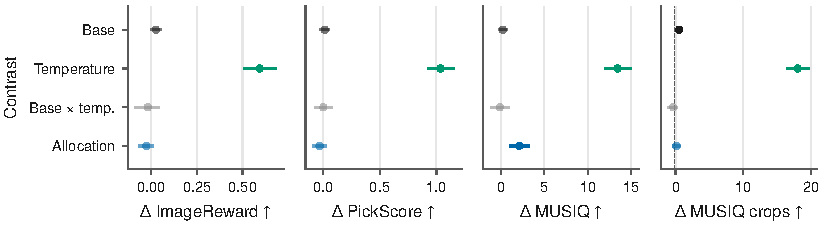
\includegraphics[width=\linewidth]{figs/strengthen/fs_factorial.pdf}
\caption{\textbf{The temperature carries the gain.} Paired contrasts on held-out rows 8 to 194 (seed 0, $n=\N{st@f@n}$): RoPE base and global temperature as main effects, their interaction, and the allocation (\segaofficial{} minus \tempsb). Whiskers are nominal 95\% intervals; marks are pale where the interval covers zero. \Cref{tab:strengthen-factorial-full} lists all ten metrics.}
\label{fig:fs-factorial}
\end{figure}

% Generated by paper/tables/strengthen_tables.py. Do not edit by hand.
\begin{table}[t]
\centering
\caption{\textbf{Factorial decomposition of \segaofficial.} Paired held-out contrasts on rows 8 to 194 ($n=187$ prompts, seed 0) from a 2$\times$2 design: RoPE base (\ntk{} or \sega) by global logit temperature (none or $s^{0.16}$), plus the allocation contrast (\segaofficial{} minus \tempsb). Main effects average the two levels of the other factor; the interaction is the temperature effect on the \sega{} base minus that on the \ntk{} base. Base, temperature and allocation add up to the whole gain of \segaofficial{} over \ntk{}. Cells give the paired mean difference with its nominal 95\% interval; triangles mark intervals that exclude zero, $^{*}$ marks Holm-adjusted $p\le0.05$ over the registered 80 tests (8 contrasts by 10 metrics), and bold marks the largest gain in each column. \Cref{tab:strengthen-factorial-full} expands this table to all eight contrasts and ten metrics. Key result: the global temperature improves all six displayed metrics under Holm (ImageReward $+0.594$, full-frame MUSIQ $+13.45$), neither the RoPE base nor the interaction survives Holm on any of the ten metrics, and the allocation improves full-frame MUSIQ ($+2.09$) while tying ImageReward and PickScore.}
\label{tab:strengthen-factorial}
\footnotesize
\setlength{\tabcolsep}{3.4pt}
% Generated by paper/tables/strengthen_tables.py. Do not edit by hand.
% Caption: \textbf{Factorial decomposition of \segaofficial.} Paired held-out contrasts (rows 8 to 194, $n=187$, seed 0) of a 2$\times$2 design, RoPE base (\ntk{} or \sega) by logit temperature (none or $s^{0.16}$), plus the allocation (\segaofficial{} minus \tempsb). Main effects average over the other factor; the interaction is the temperature effect on the \sega{} base minus that on the \ntk{} base. Base, temperature and allocation sum exactly to the total, \segaofficial{} minus \ntk, whose interval is computed directly; it is not a registered test. Cells give paired mean differences and nominal 95\% intervals; triangles mark intervals that exclude zero, $^{*}$ a Holm-adjusted $p\le0.05$ over the 80 registered tests, and bold the largest effect per column. \Cref{tab:strengthen-factorial-full} expands the table. Key result: the global temperature improves all six displayed metrics under Holm, neither the RoPE base nor the interaction survives Holm on any of the ten metrics, and the allocation improves full-frame MUSIQ ($+2.09$) while tying ImageReward and PickScore.
\begin{tabular}{@{}l rrrrrr@{}}
\toprule
Contrast & \makecell[r]{Image-\\Reward$\uparrow$} & \makecell[r]{Pick-\\Score$\uparrow$} & \makecell[r]{CLIP\\score$\uparrow$} & \makecell[r]{MUSIQ\\full$\uparrow$} & \makecell[r]{MUSIQ\\crop$\uparrow$} & \makecell[r]{CLIP-IQA\\full$\uparrow$} \\
\midrule
\multicolumn{7}{@{}l}{\emph{Main effects, averaged over the other factor}} \\
Base & \dcellT{+0.027}{-0.003}{+0.056} & \dcellT{+0.02}{-0.03}{+0.06} & \dcellT{-0.02}{-0.15}{+0.11} & \dcellT{+0.20}{-0.29}{+0.72} & \dcellB{+0.52}{+0.16}{+0.86} & \dcellT{+0.001}{-0.002}{+0.004} \\
Temperature & \dcellB{\mathbf{+0.594}^{*}}{+0.506}{+0.686} & \dcellB{\mathbf{+1.04}^{*}}{+0.92}{+1.16} & \dcellB{\mathbf{+2.03}^{*}}{+1.61}{+2.47} & \dcellB{\mathbf{+13.45}^{*}}{+11.96}{+15.11} & \dcellB{\mathbf{+18.07}^{*}}{+16.35}{+19.83} & \dcellB{\mathbf{+0.036}^{*}}{+0.021}{+0.050} \\
Base $\times$ temp. & \dcellT{-0.018}{-0.087}{+0.047} & \dcellT{+0.00}{-0.07}{+0.08} & \dcellB{+0.38}{+0.12}{+0.66} & \dcellT{-0.13}{-1.23}{+0.94} & \dcellT{-0.38}{-1.13}{+0.27} & \dcellT{-0.001}{-0.007}{+0.005} \\
\midrule
\multicolumn{7}{@{}l}{\emph{Per-band allocation}} \\
Allocation & \dcellT{-0.026}{-0.068}{+0.014} & \dcellT{-0.03}{-0.09}{+0.03} & \dcellT{-0.02}{-0.23}{+0.19} & \dcellB{+2.09^{*}}{+0.97}{+3.25} & \dcellT{+0.11}{-0.48}{+0.71} & \dcellB{+0.009}{+0.001}{+0.018} \\
\midrule
Total & \dcellB{+0.594}{+0.497}{+0.695} & \dcellB{+1.02}{+0.90}{+1.15} & \dcellB{+1.99}{+1.57}{+2.47} & \dcellB{+15.74}{+14.07}{+17.45} & \dcellB{+18.70}{+16.95}{+20.46} & \dcellB{+0.046}{+0.030}{+0.061} \\
\bottomrule
\end{tabular}

\end{table}


\paragraph{The temperature carries the gain, not the base}
\Cref{tab:strengthen-factorial} and \cref{fig:fs-factorial} complete the two-by-two design of RoPE base (\ntk{} or \sega) and global logit temperature (none or $s^{0.16}$) on the \N{st@f@n} held-out prompts. By construction, the two main effects and the allocation add up to the gain of \segaofficial{} over \ntk. Averaged over base, the temperature raises ImageReward by \N{st@f@d@temp@ir} \N{st@f@ci@temp@ir}, the whole \N{st@f@tot@ir} gain of \segaofficial{} over \ntk. It also raises full-frame MUSIQ by \N{st@f@d@temp@musiq} \N{st@f@ci@temp@musiq} of the \N{st@f@tot@musiq} total. Averaged over temperature, the \sega{} base changes ImageReward by \N{st@f@d@base@ir} \N{st@f@ci@base@ir} and full-frame MUSIQ by \N{st@f@d@base@musiq} \N{st@f@ci@base@musiq}. Its one nominal gain, \N{st@f@d@base@musiqc} \N{st@f@ci@base@musiqc} crop MUSIQ, does not survive Holm. The interaction survives Holm on no metric: the temperature raises ImageReward by \N{st@f@d@tempntk@ir} on the \ntk{} base and by \N{st@f@d@tempsega@ir} on the \sega{} base. Of the 80 registered tests, \N{st@f@nholm} survive Holm, \N{st@f@nholm@temp} for the temperature, \N{st@f@nholm@alloc} for the allocation, \N{st@f@nholm@base} for the base and \N{st@f@nholm@inter} for the interaction. \Cref{sec:decomp} credited base and temperature jointly; the factorial assigns that credit to the temperature.

\paragraph{The allocation moves image-quality scores, not rewards}
Within the same family, the allocation raises full-frame MUSIQ by \N{st@f@d@alloc@musiq} \N{st@f@ci@alloc@musiq} and crop CLIP-IQA by \N{st@f@d@alloc@iqac}. It also lowers the spectral slope error by \N{st@f@a@alloc@slope} and raises the tiling score by \N{st@f@a@alloc@tile}, a small loss, both surviving Holm. It ties ImageReward (\N{st@f@d@alloc@ir} \N{st@f@ci@alloc@ir}) and PickScore (\N{st@f@d@alloc@pick} \N{st@f@ci@alloc@pick}).

\paragraph{Reward and full-frame scores peak near $s^{0.16}$}
On the \sega{} base without allocation, five logit multipliers fixed before generation trace one curve on held-out rows 8 to 62 ($n=\N{st@s@n}$; \cref{tab:strengthen-sweep,fig:fs-sweep}). ImageReward is \N{st@sm@t100@ir} without temperature, \N{st@sm@t110@ir} at 1.1, \N{st@sm@tsref@ir} at $s^{0.16}$, \N{st@sm@tlogn@ir} at $\tau_N=4/3$ and \N{st@sm@t145@ir} at 1.45. No multiplier beats $s^{0.16}$ under Holm on ImageReward, PickScore or full-frame MUSIQ. Full-frame MUSIQ falls from \N{st@sm@tsref@musiq} at $s^{0.16}$ to \N{st@sm@t145@musiq} at 1.45, while crop MUSIQ rises at every step, from \N{st@sm@t100@musiqc} to \N{st@sm@t145@musiqc}. A crop-based quality score would therefore favour hotter attention than the reward models and the full-frame score do. \N{st@s@nholm} of the 40 sweep tests survive Holm.

\begin{figure}[t]
\centering
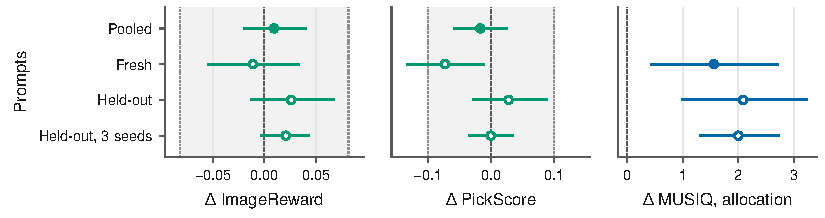
\includegraphics[width=\linewidth]{figs/strengthen/fs_confirm.pdf}
\caption{\textbf{Registered confirmation.} ImageReward and PickScore show \tempsb{} minus \segaofficial{} with the registered equivalence margins (gray band, dotted edges); full-frame MUSIQ shows the allocation (\segaofficial{} minus \tempsb). Filled marks are the registered tests (H1 on the pooled 337 prompts, H2 on the 150 fresh prompts); hollow marks are the fresh prompts alone, the held-out prompts at seed 0 and held-out prompt means over seeds 0 to 2.}
\label{fig:fs-confirm}
\end{figure}

% Generated by paper/tables/strengthen_tables.py. Do not edit by hand.
\begin{table}[!htbp]
\centering
\caption{\textbf{Registered confirmation.} $\Delta$ is \tempsb{} minus \segaofficial{} for H1 and the reverse for H2. H1 pools the 187 held-out prompts, inspected before registration, and 150 fresh prompts (seed 0) and needs both nominal intervals inside the margins and both Holm-adjusted equivalence $p\le0.05$; H2 uses the fresh prompts only and needs a positive lower bound and Holm $p\le0.05$. Holm runs over the three registered tests. The lower rows apply the same rules to the fresh prompts alone and to held-out prompt means over seeds 0 to 2, each with its own Holm family; they describe, but do not decide, the hypotheses. \Cref{tab:strengthen-fresh-arms,tab:strengthen-seeds} expand this table. Key result: H1 is supported on the pooled prompts and H2 is supported; on the fresh prompts alone the PickScore interval crosses the $-0.10$ margin, so equivalence is not established there.}
\label{tab:strengthen-fresh-tests}
\scriptsize
\setlength{\tabcolsep}{1.8pt}
% Generated by paper/tables/strengthen_tables.py. Do not edit by hand.
% Caption: \textbf{Registered confirmation.} $\Delta$ is \tempsb{} minus \segaofficial{} for H1 and the reverse for H2. H1 pools the 187 held-out and 150 fresh prompts (seed 0) and needs both nominal intervals inside the margins and both Holm-adjusted equivalence $p\le0.05$; H2 uses the fresh prompts only and needs a positive lower bound and Holm $p\le0.05$. Holm runs over the three registered tests. The lower rows apply the same rules to the fresh prompts alone and to held-out prompt means over seeds 0 to 2, each with its own Holm family; they describe, but do not decide, the hypotheses. Key result: H1 is supported on the pooled prompts and H2 is supported; on the fresh prompts alone the PickScore interval crosses the $-0.10$ margin, so equivalence is not established there.
\begin{tabular}{@{}l l r r r r l@{}}
\toprule
Test & Prompts & $\Delta$ & 95\% interval & Margin & Holm $p$ & Outcome \\
\midrule
\multicolumn{7}{@{}l}{\emph{Registered tests, one Holm family}} \\
H1 equivalence, ImageReward & 337 pooled & $+0.009$ & $[-0.020, +0.041]$ & $\pm0.082$ & $0.0015$ & \textbf{supported} \\
H1 equivalence, PickScore & 337 pooled & $-0.017$ & $[-0.059, +0.026]$ & $\pm0.100$ & $0.0015$ & \textbf{supported} \\
H2 superiority, full MUSIQ & 150 fresh & $+1.56$ & $[+0.43, +2.72]$ & $>0$ & $0.0045$ & \textbf{supported} \\
\midrule
\multicolumn{7}{@{}l}{\emph{Separately reported populations, same rules (descriptive)}} \\
H1 equivalence, ImageReward & 150 fresh & $-0.011$ & $[-0.055, +0.035]$ & $\pm0.082$ & $0.003$ & supported \\
H1 equivalence, PickScore & 150 fresh & $-0.073$ & $[-0.133, -0.011]$ & $\pm0.100$ & $0.2$ & not established \\
H1 equivalence, ImageReward & 187, 3 seeds & $+0.021$ & $[-0.004, +0.044]$ & $\pm0.082$ & $0.0015$ & supported \\
H1 equivalence, PickScore & 187, 3 seeds & $-0.000$ & $[-0.035, +0.037]$ & $\pm0.100$ & $0.0015$ & supported \\
H2 superiority, full MUSIQ & 187, 3 seeds & $+2.00$ & $[+1.30, +2.74]$ & $>0$ & $0.0015$ & supported \\
\bottomrule
\end{tabular}

\end{table}


\paragraph{Registered tests: equivalence and the MUSIQ gain hold}
H1 states that \tempsb{} is equivalent to \segaofficial{} on ImageReward (margin $\pm0.082$, half of \segaofficial's held-out gain over \dype) and on PickScore (margin $\pm0.10$). On the pooled 337 prompts the differences are \N{st@h@d@ir} \N{st@h@ci@ir} on ImageReward and \N{st@h@d@pick} \N{st@h@ci@pick} on PickScore, with Holm-adjusted equivalence $p=\N{st@h@p@ir}$ and $p=\N{st@h@p@pick}$. H2 states that the allocation raises full-frame MUSIQ on the 150 fresh prompts, where the difference is \N{st@h@d@musiq} \N{st@h@ci@musiq} (Holm $p=\N{st@h@p@musiq}$). The registered outcome is \emph{\N{st@h@H1}} for H1 and \emph{\N{st@h@H2}} for H2 (\cref{tab:strengthen-fresh-tests,fig:fs-confirm}). The pooled set reuses the 187 held-out prompts we had already inspected, so H1 extends the earlier tie rather than confirming it independently. On the fresh prompts alone, PickScore differs by \N{st@hf@d@pick} \N{st@hf@ci@pick}; this interval crosses the $-0.10$ margin, so fresh-only equivalence is \N{st@hf@status@pick}. ImageReward stays inside its margin there (\N{st@hf@d@ir} \N{st@hf@ci@ir}). We withdrew H3 before generation because its two controllers had already lost with tight intervals.

\paragraph{Fresh prompts reproduce the held-out ranking}
On the fresh prompts (\cref{tab:strengthen-fresh-arms}), ImageReward differs from \segaofficial{} by \N{st@e@d@ntk@ir} for \ntk, \N{st@e@d@segabase@ir} for the \sega{} base alone, \N{st@e@d@dype@ir} for \dype{} and \N{st@e@d@ntktemp@ir} \N{st@e@ci@ntktemp@ir} for \ntk{} with the temperature. As on the held-out set, \dype{} beats \segaofficial{} under Holm on crop MUSIQ (\N{st@e@d@dype@musiqc} \N{st@e@ci@dype@musiqc}) and CLIP-IQA (\N{st@e@d@dype@iqa}) while losing on ImageReward and PickScore (\N{st@e@d@dype@pick}). Both temperature arms trail \segaofficial{} on PickScore here, by \N{st@e@a@tsb@pick} on the \sega{} base and \N{st@e@a@ntktemp@pick} on the \ntk{} base. The held-out factorial showed no such gap, and the pooled H1 test averages over it. \N{st@e@nholm} of the 50 fresh secondary tests survive Holm.

\paragraph{Three seeds per prompt agree}
Averaging seeds 0, 1 and 2 within each held-out prompt ($n=187$ prompts, not 561 images), \tempsb{} minus \segaofficial{} is \N{st@rseeds012@d@tsb@ir} \N{st@rseeds012@ci@tsb@ir} on ImageReward, \N{st@hr@d@pick} \N{st@hr@ci@pick} on PickScore and \N{st@rseeds012@d@tsb@musiq} \N{st@rseeds012@ci@tsb@musiq} on full-frame MUSIQ (\cref{tab:strengthen-seeds}). Seeds 1 and 2 alone give \N{st@rseeds12@d@tsb@ir} \N{st@rseeds12@ci@tsb@ir} on ImageReward and \N{st@rseeds12@d@tsb@musiq} \N{st@rseeds12@ci@tsb@musiq} on full-frame MUSIQ. Each seed on its own also places the full-frame MUSIQ interval below zero.

\paragraph{The lattice is a checkpoint effect}
The dot lattice that led us to \krea{} could have come from guidance, since the earlier comparison ran \fluxdev{} at 3.5 and \krea{} at 4.5. With the official \dype{} code at matched guidance, \fluxdev{} carries \N{st@k@ratio@g3p5}$\times$ \N{st@k@ci@g3p5} the \krea{} lattice power at 3.5 and \N{st@k@ratio@g4p5}$\times$ \N{st@k@ci@g4p5} at 4.5 (8 development prompts, seed 42; \cref{tab:strengthen-ckpt}). On one bin chosen jointly for all four cells, raising guidance from 3.5 to 4.5 scales the \fluxdev{} lattice by \N{st@k@two@gdev}$\times$ \N{st@k@twoci@gdev} and the \krea{} lattice by \N{st@k@two@gkrea}$\times$ \N{st@k@twoci@gkrea}. Guidance modulates the lattice on \fluxdev, but the checkpoint gap remains at both values. \fluxdev{} also scores lower on ImageReward at both guidance values (\N{st@k@d@devminuskreag3p5@ir} at 3.5 and \N{st@k@d@devminuskreag4p5@ir} at 4.5). This is a descriptive development diagnostic.

\paragraph{The default flow shift degrades 4K samples}
The diffusers default extrapolates the flow shift to $\mu=11.55$ at $4096^2$, so the last model call sees $\sigma=\N{st@ds@sig@def}$; the official cap $\mu=1.15$ makes \N{st@ds@low@off} calls below $\sigma=0.3$ and ends at $\sigma=\N{st@ds@sig@off}$. On \N{st@ds@n} development prompts with \segaofficial{}, the default shift changes ImageReward by \N{st@ds@d@def@ir} \N{st@ds@ci@def@ir} and full-frame MUSIQ by \N{st@ds@d@def@musiq} \N{st@ds@ci@def@musiq}, and it worsens all ten metrics (\cref{tab:strengthen-default-shift}). Comparisons that mix the two schedules therefore confound the position embedding with sampling.

\paragraph{Second model family}
The registered Qwen-Image transfer test did not run. All 60 of its generation tasks failed with CUDA out-of-memory errors while a second process held about 45\,GiB of the same 95\,GiB GPU. A clean rerun did not fit the remaining compute budget. We therefore make no claim about other model families.

\subsection{Principled per-band laws do not beat \segaofficial}\label{sec:laws}

\paragraph{Outcome}
Neither law evaluated on the full held-out set improves on \segaofficial{} in any reward or image-quality metric (\cref{tab:main}, bottom block). \constancytm{} ties it on ImageReward and PickScore and is worse on CLIP (\hod{ctm}{clip}), full-frame MUSIQ (\hod{ctm}{musiq}), crop MUSIQ (\hod{ctm}{musiqc}), CLIP-IQA and the spectral error; its one gain is a lower tiling index (\hod{ctm}{tile}). It also loses to \tempsb, which shares its base and temperature and has no allocation: crop MUSIQ \hodci{ctmtsb}{musiqc} and full-frame MUSIQ \hod{ctmtsb}{musiq}, against small gains in both spectral errors (\hod{ctmtsb}{spec} and \hod{ctmtsb}{slope}). \segactm{} at $\eta=1$, the only variant to pass the campaign-2 dev gate, ties \segaofficial{} on ImageReward (\hodci{sctm}{ir}) and full-frame MUSIQ (\hodci{sctm}{musiq}) and loses on PickScore (\hodci{sctm}{pick}) and crop MUSIQ (\hodci{sctm}{musiqc}); its CLIP interval, \hoci{sctm}{clip}, ends just below zero. \aliastemp{} and \aliastemps{} failed the gate on ImageReward and were never run held out (\cref{tab:dev}); the original \constancy{} has only a partial held-out run (\cref{app:partial}). Four diagnostics, on dev prompts and on the logged gains of held-out runs, suggest possible explanations (\cref{fig:mechanism} in \cref{app:mech}). They do not identify causal mediators of image quality.


\paragraph{Diagnostic evidence}
The late-profile visibility gate stays closed through most of sampling on the development prompts. A time-matched target activates the correction earlier, but its better spectral match accompanies lower MUSIQ against the matched \tempsb{} control. The released allocation is mostly a fixed tilt; its prompt-dependent remainder also contains each prompt's noise draw and only bounds content dependence. \segactm{} increases that remainder without a held-out quality gain.

Three development probes find weak, prompt-dependent, cross-band responses. A two-prompt local linear model barely improves on no change. These probes question band-local responses without establishing a universal limit on per-band control (\cref{app:mech}).

\subsection{Checkpoint comparisons need matched settings}\label{sec:checkpoint}
% STRENGTHEN CHECKPOINT: Replace the confounded comparison only after the complete
% official-code checkpoint x guidance matrix has been verified.



Our first campaign used \fluxdev, on which \dype{} and \constancy{} produced a dense halftone lattice over the $4096^2$ frame and \ntk{} a featureless blur. An official-code \dype{} check reproduced the lattice on dev prompt 0, seed 42, at guidance 3.5; the corresponding \krea{} run at guidance 4.5 had no visible lattice (\cref{fig:checkpoint}). This rules out our port as a necessary cause of that particular failure, but the guidance difference prevents isolating the checkpoint. \dype's main reported experiments use \krea{}~\citep{issachar2025dype}, as do the official scripts we inspected. We used \krea{} for all held-out comparisons and retain the \fluxdev{} pilot as descriptive evidence only.

\subsection{\sega: paper versus code}\label{sec:papercode}

With the printed law (\cref{eq:sega,tab:papercode}), the allocation is unbounded, and at $4096^2$ the physical bin map sends every pair with a wavelength above \N{c@tokside} tokens, \N{c@collapsedpairs} of the \N{c@pairsperaxis} per axis, to the same frequency bin. The released law scales the spread by 0.15 and clamps the result at 1, and its logit gain stays between $\NmechSegaGainMin$ and $\NmechSegaGainMax$ on our held-out runs. In the eight-prompt dev pilot (descriptive only; \cref{app:pilot}), our implementation of the printed equations scores worse than the released code on every metric; freezing the printed allocation into a static tilt destroys the images, while freezing the released allocation costs much less (\cref{fig:papercode}). Readers who reimplement \sega{} from the paper will not reproduce the released method, and comparisons against \sega{} should state which version they ran.

\subsection{Pitfalls in 4K evaluation}\label{sec:pitfalls}\label{sec:spectra}

\paragraph{224-pixel scorers miss the finest octaves}
CLIP, PickScore and ImageReward see a 224-pixel view, whose Nyquist frequency is \N{nyq@cpp} cycles per original pixel ($2^{\N{nyq@log}}$); bands \N{nyq@firstband} to 10 of our 11 octave bands lie entirely above it. The methods differ in these bands (\cref{fig:spectrum_main,tab:octave}), which may help explain the reward-model ties alongside a full-frame MUSIQ gap. Resizing can retain indirect effects or alias fine patterns, but these scorers cannot directly resolve the original fine detail and are insufficient alone for 4K quality comparisons. \Cref{app:full} gives the bandwise values.

\paragraph{Attention kernel}
Attention backend and GPU can dominate method-level timing differences (\cref{app:compute}); comparisons must fix both. Our records did not log the dispatched kernel or a hash of the loaded weights. We reconstructed the configured attention policy and transformer identity from code revisions and task scripts; neither is a direct runtime record.
% STRENGTHEN QWEN: Insert complete within-family Qwen results here or in a dedicated
% appendix, including every registered arm and metric; do not compare raw rewards
% between families as checkpoint effects.

\section{Related work}\label{sec:related}

\paragraph{Training-free high-resolution generation}
U-Net methods modify convolutional scale~\citep{he2024scalecrafter,huang2024fouriscale}, fuse patches or scales~\citep{du2024demofusion,qiu2024freescale}, restructure features~\citep{zhang2024hidiffusion} or cascade over frequencies~\citep{zhang2025frecas}. For flow transformers~\citep{peebles2023dit,esser2024sd3,flux2024}, I-Max and HiFlow guide generation with a low-resolution trajectory~\citep{du2024imax,bu2025hiflow}; HRDiT adapts pretrained transformers~\citep{hrdit2026}, and Diffusion-4K fine-tunes at 4K and supplies our prompts~\citep{zhang2025diffusion4k}. We study embedding changes that add neither training nor sampling passes.

\paragraph{Rotary extrapolation and attention temperature}
Interpolation, NTK scaling, YaRN and LongRoPE remap rotary frequencies~\citep{chen2023pi,bloc97ntk,peng2024yarn,ding2024longrope}; frequency analyses separate positional and semantic roles~\citep{barbero2025round,xiong2025dope}. In diffusion, RIFLEx targets video repetition~\citep{zhao2025riflex}, \dype{} schedules remapping~\citep{issachar2025dype}, UltraImage selects frequencies~\citep{ultraimage2025}, TIDE controls temperature~\citep{tide2026}, \sega{} adds per-band gains~\citep{sega2026} and AReA adapts locality~\citep{area2026}. Log-key-count temperature scaling is established in variable-size diffusion and Scalable-Softmax~\citep{jin2023training,nakanishi2025ssmax}; we test its contribution together with the base.

\paragraph{Spectral views and efficient coding}
Coarse-to-fine denoising and harmonic adaptation motivate spectral analyses~\citep{dieleman2024spectral,falck2025fourier,kadkhodaie2024generalization,graikos2026jacobian}. Existing interventions target spectra~\citep{scg2026}, weight training by contrast sensitivity~\citep{csflow2026} or edit cross-attention Fourier bands~\citep{oh2026afm}. Our rotary-band controllers draw on natural-image spectra~\citep{field1987relations,dong1995statistics}, human sensitivity~\citep{knill1990human,parraga2000human}, efficient coding~\citep{atick1990towards,atick1992retina,vanhateren1992theory}, contrast constancy~\citep{georgeson1975contrast} and divisive gain control~\citep{webster2002neural,heeger1992normalization,schwartz2001natural,carandini2012normalization}.

\section{Discussion}\label{sec:discussion}

\paragraph{What to report}
A method that changes the rotary base, the temperature and per-band gains at once should report a control that keeps its base and temperature and drops the rest, and it should separate base from temperature. Here the temperature alone carries the reward-model gain; one untested explanation is that softmax attention spreads over \N{c@tokratio} times more keys and a multiplier above 1 sharpens it again~\citep{jin2023training}. The allocation adds \N{st@h@a@musiq} \N{st@h@ci@musiq} full-frame MUSIQ points on fresh prompts with no Holm-surviving reward-model gain, and its lower excess fine-scale power does not establish a perceptual mechanism. Claims that credit spectral or content adaptivity should be tested against this control with full-resolution metrics (\cref{sec:pitfalls}), using the code released with this paper.

\section{Limitations}\label{sec:limitations}
% One paragraph of scoped limits, as in the gold-standard papers (2026-10-24; was a six-item list).
\textbf{One model and size.} Only \krea{} at $4096^2$; the registered \qwen{} test ran out of GPU memory, so other backbones, shapes and video are untested. \textbf{Reused prompts and few seeds.} H1 pools \N{st@f@n} already inspected held-out prompts with \N{st@e@n} fresh ones; on the fresh prompts alone PickScore equivalence is not established (\N{st@hf@d@pick} \N{st@hf@ci@pick}). Two arms have three seeds, the rest one, and all prompts are \afk{} captions. \textbf{Automatic metrics.} The reward models see 224 pixels, MUSIQ and CLIP-IQA are learned proxies, the spectral error uses a mean reference profile, and we ran no human study. \textbf{Multiplicity.} Holm covers each registered family and, retrospectively, the main tables. Intervals are nominal, \cref{tab:deltas_full} alone holds \N{ho@ncomp} comparisons, and no correction spans all tables. \textbf{Small diagnostic samples.} \constancy{} ran on part of the held-out set; the pilot and the checkpoint and flow-shift controls use 8 dev prompts, and mechanism probes at most three. \textbf{Ports.} We port \sega{} and \dype{} with parity tests against their code, ran official \dype{} code only for the checkpoint control, and lack the \sega{} authors' confirmation of our reading.

\section*{Reproducibility statement}\label{sec:repro}
\Cref{sec:protocol} fixes prompts, split, seeds, sampler and statistics. \Cref{app:impl} gives the pipeline, software versions, MUSIQ inputs, pinned \sega{} and \dype{} commits and every arm's formula (\cref{tab:methods}), and \cref{app:laws} the control laws and calibration. \Cref{app:full,app:seed1} expand every main table to all ten metrics with intervals and Holm marks; \cref{app:partial} lists dev-selection decisions, \cref{app:mech} the diagnostic protocols, \cref{app:compute} the sampling cost and \cref{app:repro} the scripts behind each number. Code and per-image scores are at \codeurl.


\clearpage
{\small
\setlength{\bibsep}{1.5pt plus 0.3pt}
\bibliographystyle{plainnat}
\bibliography{refs}
}

\clearpage
\appendix
\counterwithin{figure}{section}
\counterwithin{table}{section}
\section*{Appendix contents}
\startcontents[app]
\printcontents[app]{l}{1}{\setcounter{tocdepth}{1}}
\section{Additional figures}\label{app:figs}

This appendix expands \cref{fig:qual_main,fig:spectrum_main} and holds the development figures behind \cref{sec:checkpoint,sec:papercode}. \Cref{fig:qual} shows held-out samples, \cref{fig:checkpoint} the development checkpoint diagnostic, \cref{fig:spectrum} the octave-band spectra, and \cref{fig:papercode} the development paper-versus-code comparison.

\begin{figure}[H]
\centering
\figorplaceholder[\linewidth]{figs/f4_qualitative.pdf}{3.1in}
\caption{\textbf{\ntk{} loses fine detail at $4096^2$.} The other arms render comparable detail, and \dype{} shows faint speckle in flat sky on held-out row 8 (one crop checked); compositions differ between arms, so a crop can show different content. Held-out rows 8, 9 and 10 (left to right), the first three held-out rows, were fixed before any output was viewed; seed 0, one sample per arm. Full frames are Lanczos-reduced; native-resolution crops sit at identical coordinates and are never resampled (red: highest-detail tile of the across-arm mean luminance; cyan: image center). Prompts, left to right: ``A stone bridge with arched spans reflects golden light on the water, flanked by buildings and a leafy tree under a clear blue sky.'' ``A panoramic view of Paris featuring the Eiffel Tower, the Seine River, and various ornate buildings with greenery and bustling activity, including boats on the water and crowds along walkways.'' ``A cluttered artist's corner features an ornate gold frame, a painting of a man with glasses, several empty picture frames, a vintage suitcase, and various brushes in a tin can, all set against a textured gray wall and draped with patterned fabric.''}
\label{fig:qual}
\end{figure}

\begin{figure}[H]
\centering
\figorplaceholder[\linewidth]{figs/f5_checkpoint.pdf}{3.26in}
\caption{\textbf{Lattice and checkpoint check.} The development comparison shows a lattice on \fluxdev{}, but checkpoint and guidance both change. (a)~Dev prompt 0 under official \dype{} code (seed 42) and our \dype{} and \segaofficial{} pipelines (seed 0), at guidance 3.5 (\fluxdev) and 4.5 (\krea). Red and cyan boxes mark native 192-pixel windows at the same place in every image. (b)~Whitened radial power spectra of luminance: \fluxdev{} (black) peaks at the lattice period (dot) and \krea{} (gray) does not in these samples. Peak ratios: 36$\times$ for the official-code pair; over eight prompts in our pipeline, 12$\times$ [7, 20] for \dype{} and 5$\times$ [2, 11] for \segaofficial{} (geometric means, 95\% bootstrap intervals). Official-code evidence covers one prompt per checkpoint, and the figure does not isolate a checkpoint effect.}
\label{fig:checkpoint}
\end{figure}

\begin{figure}[H]
\centering
\figorplaceholder[\linewidth]{figs/f8_spectrum.pdf}{2.2in}
\caption{\textbf{Spectra against references and \sega.} Without \sega's per-band allocation, luminance power at 8 to 32 pixel wavelengths (gray band) sits above released \sega's; \constancytm{} leaves a similar excess, and \ntk{} falls short from 8 to 1024 pixels. (a)~Log-power error against the mean $\ln P$ of the 195 \afk{} references, per octave band of linear-sRGB luminance; (b)~paired difference from \segaofficial, the dashed blue zero line; positive means more power. Held-out rows 8--194 ($n=\N{ho@nprompts}$, seed 0) with 95\% bootstrap intervals over prompts; the dashed vertical marks the Nyquist frequency of a 224-pixel view.}
\label{fig:spectrum}
\end{figure}

\begin{figure}[H]
\centering
\figorplaceholder[\linewidth]{figs/f6_sega_code.pdf}{2.4in}
\caption{\textbf{Printed equations against the release.} The printed-law implementation produces larger gain changes than the release and degrades this development pilot. Eight dev prompts (rows 0--7, seed 0), descriptive only. (a)~Median log logit gain per rotary pair (pair 0 has the highest frequency) and denoising step. Released and printed-law heatmaps have separate symmetric color scales, so equal colors across the groups do not mean equal magnitudes. The line panel uses one shared axis for mean log gain over prompts, steps and both spatial axes; static variants (dashed) average each method's gains over prompts and steps. (b)~Dev prompt 0, seed 0: full frames and a native-resolution crop (red box). \Cref{tab:papercode_scores} gives CLIP score and ImageReward means over the eight dev prompts, with paired differences from \segaofficial{} and 95\% bootstrap intervals.}
\label{fig:papercode}
\end{figure}

\clearpage

\section{Full held-out results}\label{app:full}

This appendix expands \cref{tab:results}: \cref{tab:main} gives its paired differences with intervals, \cref{tab:share} the decomposition with means, \cref{tab:means_full,tab:deltas_full} all ten metrics and \cref{tab:octave} the spectral bands.

\begin{table}[!htbp]
\centering
\caption{\textbf{Paired held-out differences (expands \cref{tab:results}).} Held-out paired differences against \segaofficial{} (rows 8--194, seed 0, $n=\N{ho@nprompts}$); the first row gives the absolute means of \segaofficial. Each cell shows the mean difference and its nominal 95\% bootstrap interval; \better{}/\worse{} mark intervals that exclude zero in the better or worse direction; unmarked cells are ties. A star marks a Holm-adjusted $p\le0.05$ across this table's paired comparisons, using approximate centered-bootstrap tests. \Cref{tab:deltas_full} has all ten metrics and a separate Holm family. Key result: base and temperature carry most of \sega's gain, and no per-band law beats it.}
\label{tab:main}
\footnotesize
\setlength{\tabcolsep}{3.1pt}
\begin{tabular}{@{}l rrrrrr@{}}
\toprule
Method & \makecell[r]{Image-\\Reward$\uparrow$} & \makecell[r]{Pick-\\Score$\uparrow$} & \makecell[r]{CLIP\\score$\uparrow$} & \makecell[r]{MUSIQ\\full$\uparrow$} & \makecell[r]{MUSIQ\\crop$\uparrow$} & \makecell[r]{CLIP-IQA\\full$\uparrow$} \\
\midrule
\segaofficial{} & \refcell{1.190} & \refcell{23.05} & \refcell{29.14} & \refcell{45.23} & \refcell{58.33} & \refcell{0.603} \\
\midrule
\multicolumn{7}{@{}l}{\emph{Decomposition of \segaofficial}} \\[1pt]
\ntk{} & \dcellW{-0.594}{-0.701}{-0.494} & \dcellW{-1.02}{-1.16}{-0.89} & \dcellW{-1.99}{-2.43}{-1.55} & \dcellW{-15.74}{-17.50}{-14.00} & \dcellW{-18.70}{-20.68}{-16.86} & \dcellW{-0.046}{-0.062}{-0.031} \\
\tempsb{} & \dcellT{+0.026}{-0.016}{+0.070} & \dcellT{+0.03}{-0.03}{+0.09} & \dcellT{+0.02}{-0.19}{+0.23} & \dcellW{-2.09}{-3.25}{-0.96} & \dcellT{-0.11}{-0.71}{+0.51} & \dcellW{-0.009}{-0.018}{-0.001} \\
\addlinespace[2pt]
\multicolumn{7}{@{}l}{\emph{Other baseline}} \\[1pt]
\dype{} & \dcellW{-0.164}{-0.258}{-0.087} & \dcellW{-0.49}{-0.63}{-0.36} & \dcellW{-0.37}{-0.72}{-0.01} & \dcellW{-1.88}{-3.26}{-0.56} & \dcellB{+1.97}{+1.16}{+2.80} & \dcellB{+0.029}{+0.020}{+0.038} \\
\addlinespace[2pt]
\multicolumn{7}{@{}l}{\emph{Principled per-band laws (ours)}} \\[1pt]
\constancytm{} & \dcellT{+0.018}{-0.023}{+0.059} & \dcellT{-0.05}{-0.11}{+0.02} & \dcellW{-0.27}{-0.49}{-0.04} & \dcellW{-3.04}{-4.28}{-1.81} & \dcellW{-2.19}{-2.81}{-1.57} & \dcellW{-0.025}{-0.034}{-0.017} \\
\segactm{} & \dcellT{+0.009}{-0.008}{+0.027} & \dcellW{-0.08}{-0.10}{-0.05} & \dcellW{-0.09}{-0.20}{+0.00} & \dcellT{-0.21}{-0.71}{+0.32} & \dcellW{-1.13}{-1.39}{-0.90} & \dcellT{+0.003}{+0.000}{+0.006} \\
\bottomrule
\end{tabular}

\end{table}

\Cref{tab:share} decomposes \sega's gain over \ntk{} with means and paired gains, \cref{tab:means_full} gives absolute means and \cref{tab:deltas_full} the paired differences for all ten metrics. The spectral rows use the mean octave profile of the 195 \afk{} reference images as the target; \cref{tab:octave} breaks the spectral error into its 11 octave bands. FID and KID are not tabulated: for the seed-1 images (\N{fid@n} prompts per arm, including one dev row), the paired FID difference of \tempsb{} against \segaofficial{} is \N{fid@tsb@fid} with interval \N{fid@tsb@fid@ci}, and that of \constancytm{} is \N{fid@ctm@fid} with interval \N{fid@ctm@fid@ci}.

In band 7, \ntk{} falls below the reference profile (log-power error \N{oct@ntk@b7}); the two arms with \sega's allocation stay closest to it (\segaofficial{} \N{oct@sega@b7}, \segactm{} \N{oct@sctm@b7}), and \tempsb{} carries excess power (\N{oct@tsb@b7}). These held-out spectral differences lie above the Nyquist limit of the 224-pixel reward-model view (\cref{sec:pitfalls}).

\begin{table}[!htbp]
\centering
\caption{\textbf{Where \sega's improvement over \ntk{} comes from.} Means on the same \N{sh@n} held-out prompts, paired gains from base and temperature and from the allocation, and the share of the total gain carried by base and temperature, (\tempsb{} $-$ \ntk)/(\segaofficial{} $-$ \ntk), with its 95\% paired bootstrap interval. A share above 100\% means the allocation's point estimate is negative.}
\label{tab:share}
\footnotesize
\setlength{\tabcolsep}{4pt}
\begin{tabular}{@{}l rrr rr r@{}}
\toprule
 & \multicolumn{3}{c}{Mean ($n=187$)} & \multicolumn{2}{c}{Paired gain} & \\
\cmidrule(lr){2-4}\cmidrule(lr){5-6}
Metric & \ntkH & \tempsbH & \segaofficialH & \hdr{base\\+\,temp.} & \hdr{alloc-\\ation} & \hdr{share of\\base\,+\,temp.} \\
\midrule
ImageReward$\uparrow$ & $0.596$ & $1.216$ & $1.190$ & \dcellB{+0.620}{+0.525}{+0.724} & \dcellT{-0.026}{-0.070}{+0.016} & 104\% {\fontsize{6.5}{7}\selectfont[97, 113]} \\
PickScore$\uparrow$ & $22.03$ & $23.08$ & $23.05$ & \dcellB{+1.05}{+0.92}{+1.18} & \dcellT{-0.03}{-0.09}{+0.03} & 103\% {\fontsize{6.5}{7}\selectfont[97, 109]} \\
CLIP$\uparrow$ & $27.15$ & $29.15$ & $29.14$ & \dcellB{+2.01}{+1.57}{+2.48} & \dcellT{-0.02}{-0.23}{+0.19} & 101\% {\fontsize{6.5}{7}\selectfont[90, 112]} \\
MUSIQ$\uparrow$ & $29.49$ & $43.14$ & $45.23$ & \dcellB{+13.65}{+12.05}{+15.28} & \dcellB{+2.09}{+0.96}{+3.25} & 87\% {\fontsize{6.5}{7}\selectfont[80, 94]} \\
MUSIQ\textsubscript{crop}$\uparrow$ & $39.63$ & $58.22$ & $58.33$ & \dcellB{+18.59}{+16.72}{+20.63} & \dcellT{+0.11}{-0.51}{+0.71} & 99\% {\fontsize{6.5}{7}\selectfont[96, 103]} \\
CLIP-IQA$\uparrow$ & $0.557$ & $0.594$ & $0.603$ & \dcellB{+0.037}{+0.021}{+0.053} & \dcellB{+0.009}{+0.001}{+0.018} & 80\% {\fontsize{6.5}{7}\selectfont[59, 98]} \\
\bottomrule
\end{tabular}

\end{table}

\begin{table}[!htbp]
\centering
\caption{\textbf{Held-out means with 95\% bootstrap intervals} (rows 8--194, seed 0). \constancy{} is the partial run on \hon{cons} prompts (\cref{app:partial}).}
\label{tab:means_full}
\scriptsize
\setlength{\tabcolsep}{1.3pt}
\begin{tabular}{@{}lrrrrrrr@{}}
\toprule
Metric & \segaofficialH & \ntkH & \tempsbH & \dypeH & \constancyH & \constancytmH & \segactmH \\
 & \tiny $n=187$ & \tiny $n=187$ & \tiny $n=187$ & \tiny $n=187$ & \tiny $n=41$ & \tiny $n=187$ & \tiny $n=187$ \\
\midrule
ImageReward$\uparrow$ & \mcell{1.190}{1.087}{1.284} & \mcell{0.596}{0.456}{0.736} & \mcell{1.216}{1.118}{1.313} & \mcell{1.026}{0.910}{1.142} & \mcell{1.177}{0.953}{1.392} & \mcell{1.208}{1.110}{1.304} & \mcell{1.199}{1.096}{1.293} \\
PickScore$\uparrow$ & \mcell{23.05}{22.89}{23.21} & \mcell{22.03}{21.84}{22.21} & \mcell{23.08}{22.92}{23.24} & \mcell{22.57}{22.36}{22.75} & \mcell{22.70}{22.29}{23.08} & \mcell{23.01}{22.84}{23.16} & \mcell{22.98}{22.81}{23.13} \\
CLIP$\uparrow$ & \mcell{29.14}{28.70}{29.55} & \mcell{27.15}{26.64}{27.64} & \mcell{29.15}{28.72}{29.58} & \mcell{28.76}{28.32}{29.20} & \mcell{29.46}{28.40}{30.49} & \mcell{28.87}{28.42}{29.31} & \mcell{29.04}{28.61}{29.47} \\
MUSIQ$\uparrow$ & \mcell{45.23}{43.69}{46.79} & \mcell{29.49}{28.13}{30.95} & \mcell{43.14}{41.58}{44.61} & \mcell{43.35}{41.71}{45.02} & \mcell{40.55}{37.20}{43.56} & \mcell{42.19}{40.65}{43.58} & \mcell{45.02}{43.56}{46.53} \\
MUSIQ\textsubscript{crop}$\uparrow$ & \mcell{58.33}{57.06}{59.63} & \mcell{39.63}{37.77}{41.33} & \mcell{58.22}{57.07}{59.44} & \mcell{60.30}{59.12}{61.53} & \mcell{60.75}{58.19}{63.01} & \mcell{56.14}{54.98}{57.36} & \mcell{57.20}{55.84}{58.52} \\
CLIP-IQA$\uparrow$ & \mcell{0.603}{0.590}{0.616} & \mcell{0.557}{0.546}{0.568} & \mcell{0.594}{0.581}{0.607} & \mcell{0.632}{0.618}{0.645} & \mcell{0.572}{0.544}{0.601} & \mcell{0.578}{0.566}{0.590} & \mcell{0.606}{0.593}{0.619} \\
CLIP-IQA\textsubscript{crop}$\uparrow$ & \mcell{0.586}{0.573}{0.600} & \mcell{0.537}{0.525}{0.549} & \mcell{0.569}{0.556}{0.583} & \mcell{0.599}{0.585}{0.613} & \mcell{0.543}{0.514}{0.572} & \mcell{0.550}{0.538}{0.563} & \mcell{0.588}{0.576}{0.602} \\
Spec.\ err.$\downarrow$ & \mcell{1.068}{1.005}{1.133} & \mcell{1.285}{1.214}{1.358} & \mcell{1.102}{1.035}{1.168} & \mcell{1.096}{1.024}{1.168} & \mcell{1.337}{1.205}{1.477} & \mcell{1.088}{1.020}{1.152} & \mcell{1.066}{1.001}{1.133} \\
Slope err.$\downarrow$ & \mcell{0.200}{0.180}{0.221} & \mcell{0.165}{0.146}{0.185} & \mcell{0.224}{0.200}{0.247} & \mcell{0.218}{0.194}{0.242} & \mcell{0.276}{0.218}{0.338} & \mcell{0.218}{0.195}{0.240} & \mcell{0.197}{0.178}{0.218} \\
Tiling$\downarrow$ & \mcell{0.0684}{0.0568}{0.0802} & \mcell{0.0757}{0.0612}{0.0905} & \mcell{0.0616}{0.0507}{0.0732} & \mcell{0.0865}{0.0778}{0.0953} & \mcell{0.0589}{0.0390}{0.0797} & \mcell{0.0616}{0.0505}{0.0732} & \mcell{0.0684}{0.0566}{0.0804} \\
\bottomrule
\end{tabular}

\end{table}

\begin{table}[!htbp]
\centering
\caption{\textbf{Held-out paired differences against \segaofficial{}, all metrics.} Nominal 95\% intervals and direction triangles as in \cref{tab:main}; stars mark approximate Holm-adjusted $p\le0.05$ across all paired comparisons in this table. \constancy{} is the partial run on \hon{cons} prompts (\cref{app:partial}).}
\label{tab:deltas_full}
\scriptsize
\setlength{\tabcolsep}{1.8pt}
\begin{tabular}{@{}lrrrrrr@{}}
\toprule
Metric & \ntkH & \tempsbH & \dypeH & \constancyH & \constancytmH & \segactmH \\
 & \tiny $n=187$ & \tiny $n=187$ & \tiny $n=187$ & \tiny $n=41$ & \tiny $n=187$ & \tiny $n=187$ \\
\midrule
ImageReward$\uparrow$ & \dcellW{-0.594}{-0.701}{-0.494} & \dcellT{+0.026}{-0.016}{+0.070} & \dcellW{-0.164}{-0.258}{-0.087} & \dcellT{+0.018}{-0.089}{+0.133} & \dcellT{+0.018}{-0.023}{+0.059} & \dcellT{+0.009}{-0.008}{+0.027} \\
PickScore$\uparrow$ & \dcellW{-1.02}{-1.16}{-0.89} & \dcellT{+0.03}{-0.03}{+0.09} & \dcellW{-0.49}{-0.63}{-0.36} & \dcellT{-0.07}{-0.28}{+0.18} & \dcellT{-0.05}{-0.11}{+0.02} & \dcellW{-0.08}{-0.10}{-0.05} \\
CLIP$\uparrow$ & \dcellW{-1.99}{-2.43}{-1.55} & \dcellT{+0.02}{-0.19}{+0.23} & \dcellW{-0.37}{-0.72}{-0.01} & \dcellT{-0.05}{-0.78}{+0.68} & \dcellW{-0.27}{-0.49}{-0.04} & \dcellW{-0.09}{-0.20}{+0.00} \\
MUSIQ$\uparrow$ & \dcellW{-15.74}{-17.50}{-14.00} & \dcellW{-2.09}{-3.25}{-0.96} & \dcellW{-1.88}{-3.26}{-0.56} & \dcellW{-5.09}{-8.44}{-1.74} & \dcellW{-3.04}{-4.28}{-1.81} & \dcellT{-0.21}{-0.71}{+0.32} \\
MUSIQ\textsubscript{crop}$\uparrow$ & \dcellW{-18.70}{-20.68}{-16.86} & \dcellT{-0.11}{-0.71}{+0.51} & \dcellB{+1.97}{+1.16}{+2.80} & \dcellB{+1.91}{+0.10}{+3.80} & \dcellW{-2.19}{-2.81}{-1.57} & \dcellW{-1.13}{-1.39}{-0.90} \\
CLIP-IQA$\uparrow$ & \dcellW{-0.046}{-0.062}{-0.031} & \dcellW{-0.009}{-0.018}{-0.001} & \dcellB{+0.029}{+0.020}{+0.038} & \dcellT{-0.005}{-0.031}{+0.019} & \dcellW{-0.025}{-0.034}{-0.017} & \dcellT{+0.003}{+0.000}{+0.006} \\
CLIP-IQA\textsubscript{crop}$\uparrow$ & \dcellW{-0.049}{-0.066}{-0.034} & \dcellW{-0.017}{-0.026}{-0.008} & \dcellB{+0.013}{+0.003}{+0.023} & \dcellT{-0.027}{-0.053}{+0.001} & \dcellW{-0.036}{-0.045}{-0.027} & \dcellT{+0.002}{-0.001}{+0.006} \\
Spec.\ err.$\downarrow$ & \dcellW{+0.216}{+0.154}{+0.287} & \dcellW{+0.034}{+0.016}{+0.051} & \dcellT{+0.028}{-0.007}{+0.061} & \dcellW{+0.204}{+0.127}{+0.277} & \dcellW{+0.019}{+0.001}{+0.037} & \dcellT{-0.002}{-0.009}{+0.004} \\
Slope err.$\downarrow$ & \dcellB{-0.035}{-0.053}{-0.018} & \dcellW{+0.024}{+0.013}{+0.034} & \dcellW{+0.018}{+0.003}{+0.033} & \dcellW{+0.061}{+0.021}{+0.101} & \dcellW{+0.018}{+0.008}{+0.027} & \dcellT{-0.003}{-0.007}{+0.002} \\
Tiling$\downarrow$ & \dcellT{+0.0074}{-0.0044}{+0.0185} & \dcellB{-0.0068}{-0.0108}{-0.0026} & \dcellW{+0.0182}{+0.0085}{+0.0279} & \dcellT{-0.0099}{-0.0223}{+0.0041} & \dcellB{-0.0068}{-0.0107}{-0.0026} & \dcellT{+0.0001}{-0.0007}{+0.0008} \\
\bottomrule
\end{tabular}

\end{table}

\begin{table}[!htbp]
\centering
\caption{\textbf{Spectral error by octave band.} Mean log-power difference from the \afk{} reference profile on held-out prompts; positive values mean excess power. Bands \N{nyq@firstband} to 10 lie above the Nyquist frequency of a 224-pixel view of a $4096^2$ image. \constancy{} is the partial run on \hon{cons} prompts (\cref{app:partial}).}
\label{tab:octave}
\scriptsize
\setlength{\tabcolsep}{2.6pt}
\begin{tabular}{@{}lrrrrrrrrrrr@{}}
\toprule
Octave band & 0 & 1 & 2 & 3 & 4 & 5 & 6 & 7 & 8 & 9 & 10 \\
Centre (cyc/px) & \tiny $2^{-12.5}$ & \tiny $2^{-11.5}$ & \tiny $2^{-10.5}$ & \tiny $2^{-9.5}$ & \tiny $2^{-8.5}$ & \tiny $2^{-7.5}$ & \tiny $2^{-6.5}$ & \tiny $2^{-5.5}$ & \tiny $2^{-4.5}$ & \tiny $2^{-3.5}$ & \tiny $2^{-2.5}$ \\
\midrule
\segaofficial & $+0.85$ & $+0.34$ & $+0.09$ & $-0.05$ & $-0.18$ & $-0.17$ & $-0.10$ & $+0.06$ & $+0.44$ & $+1.15$ & $+0.93$ \\
\ntk & $+0.53$ & $+0.02$ & $-0.47$ & $-0.77$ & $-1.03$ & $-1.16$ & $-1.20$ & $-1.30$ & $-1.16$ & $+0.43$ & $+1.15$ \\
\tempsb & $+0.75$ & $+0.25$ & $+0.02$ & $-0.10$ & $-0.21$ & $-0.15$ & $+0.04$ & $+0.39$ & $+0.78$ & $+1.27$ & $+1.10$ \\
\dype & $+0.70$ & $-0.02$ & $+0.01$ & $+0.04$ & $+0.07$ & $+0.07$ & $+0.19$ & $+0.42$ & $+0.71$ & $+1.17$ & $+1.09$ \\
\constancy & $+0.73$ & $+0.34$ & $+0.27$ & $+0.23$ & $+0.21$ & $+0.36$ & $+0.72$ & $+1.37$ & $+1.72$ & $+1.84$ & $+1.64$ \\
\constancytm & $+0.74$ & $+0.24$ & $+0.01$ & $-0.12$ & $-0.23$ & $-0.19$ & $+0.00$ & $+0.36$ & $+0.72$ & $+1.17$ & $+0.96$ \\
\segactm & $+0.84$ & $+0.34$ & $+0.08$ & $-0.06$ & $-0.20$ & $-0.20$ & $-0.14$ & $-0.01$ & $+0.33$ & $+1.04$ & $+0.82$ \\
\bottomrule
\end{tabular}

\end{table}

\FloatBarrier
% Generated by paper/tables/strengthen_tables.py. Do not edit by hand.
\section{Confirmation campaign: full tables}\label{app:confirm}
This appendix expands \cref{sec:confirm}. \Cref{tab:strengthen-factorial-full} expands \cref{tab:strengthen-factorial} to all eight contrasts and ten metrics; \cref{tab:strengthen-factorial-means} gives the factorial cell means; \cref{tab:strengthen-sweep,fig:fs-sweep} give the temperature sweep; \cref{tab:strengthen-fresh-arms} compares every fresh-prompt arm with \segaofficial; \cref{tab:strengthen-seeds} gives the seed replication; \cref{tab:strengthen-ckpt} the checkpoint-by-guidance lattice; \cref{tab:strengthen-default-shift} the default flow shift. Every table lists all registered metrics, including unfavourable ones, with nominal 95\% paired prompt-bootstrap intervals (2{,}000 draws, seed 0).

% Generated by paper/tables/strengthen_tables.py. Do not edit by hand.
\begin{table}[!htbp]
\centering
\caption{\textbf{All factorial contrasts.} Every registered contrast and metric of the held-out factorial ($n=187$, seed 0), with the same cells, marks and Holm family as \cref{tab:strengthen-factorial}, transposed; bold marks the largest gain for each metric. Key result: 31 of 80 tests survive Holm: 27 temperature tests (every metric except tiling) and 4 allocation tests (better on full-frame MUSIQ, crop CLIP-IQA and slope error; worse on tiling); neither the RoPE base nor the interaction survives Holm on any of the ten metrics.}
\label{tab:strengthen-factorial-full}
\scriptsize
\setlength{\tabcolsep}{1.8pt}
\input{tables/tab_strengthen_factorial_full.tex}
\end{table}

% Generated by paper/tables/strengthen_tables.py. Do not edit by hand.
\begin{table}[!htbp]
\centering
\caption{\textbf{Factorial cell means.} Held-out means ($n=187$, seed 0) of the four base-by-temperature cells and of \segaofficial{}, in the shaded column; the first two columns have no temperature. Bold is best and underlined second for each metric among the displayed rounded values; the paired tests are in \cref{tab:strengthen-factorial}. Key result: Each of the three arms with the temperature scores better than both arms without it on every metric except slope error.}
\label{tab:strengthen-factorial-means}
\scriptsize
\setlength{\tabcolsep}{1.8pt}
\input{tables/tab_strengthen_factorial_means.tex}
\end{table}

% Generated by paper/tables/strengthen_tables.py. Do not edit by hand.
\begin{table}[!htbp]
\centering
\caption{\textbf{Global temperature sweep.} \tempsb{} with the logit multiplier fixed in advance at five values, held-out rows 8 to 62 ($n=55$, seed 0, the first 55 held-out rows of the manifest). The shaded column is \sega's reference $s^{0.16}=1.248$ and shows means; other columns show the paired difference from it with nominal 95\% intervals; $^{*}$ marks Holm-adjusted $p\le0.05$ over 40 tests (4 settings by 10 metrics). Bold marks the best setting for a metric when its interval separates it from the reference. No value was selected from these results. Key result: Removing the temperature (1.000) worsens all six displayed metrics under Holm (ImageReward $-0.671$); no multiplier beats $s^{0.16}$ under Holm on ImageReward, PickScore or full-frame MUSIQ, whereas crop MUSIQ rises monotonically with the multiplier, from 40.12 at 1.000 to 65.87 at 1.450.}
\label{tab:strengthen-sweep}
\scriptsize
\setlength{\tabcolsep}{1.8pt}
\input{tables/tab_strengthen_sweep.tex}
\end{table}

\begin{figure}[!htbp]
\centering
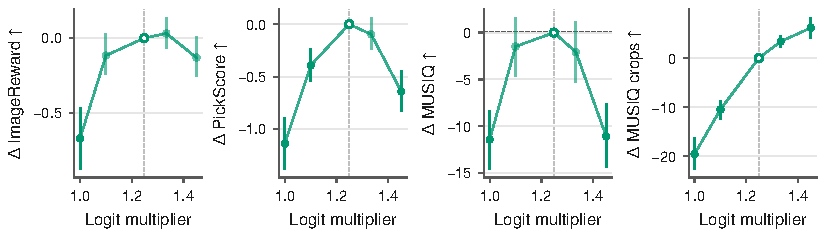
\includegraphics[width=\linewidth]{figs/strengthen/fs_sweep.pdf}
\caption{\textbf{Temperature sweep.} \tempsb{} at five logit multipliers fixed before generation, minus the reference $s^{0.16}$ (hollow mark, dashed vertical), on held-out rows 8 to 62 ($n=\N{st@s@n}$, seed 0). Whiskers are nominal 95\% paired intervals; pale marks cover zero. Reward models and full-frame MUSIQ fall on both sides of $s^{0.16}$, while crop MUSIQ keeps rising with the multiplier.}
\label{fig:fs-sweep}
\end{figure}
% Generated by paper/tables/strengthen_tables.py. Do not edit by hand.
\begin{table}[!htbp]
\centering
\caption{\textbf{Fresh prompts.} Means of \segaofficial{}, in the shaded column, and paired differences from it on 150 unseen Aesthetic-4K training captions ($n=150$, seed 0), with nominal 95\% intervals; $^{*}$ marks Holm-adjusted $p\le0.05$ over 50 tests (5 arms by 10 metrics). Bold marks the best entry for a metric when its interval separates it from \segaofficial. Key result: \dype{} is the only arm that beats \segaofficial{} under Holm on crop MUSIQ ($+2.32$) and CLIP-IQA ($+0.024$) while losing ImageReward ($-0.166$) and PickScore ($-0.38$); \tempsb{} ties ImageReward ($-0.011$) and loses crop CLIP-IQA and slope error under Holm.}
\label{tab:strengthen-fresh-arms}
\scriptsize
\setlength{\tabcolsep}{1.8pt}
\input{tables/tab_strengthen_fresh_arms.tex}
\end{table}

% Generated by paper/tables/strengthen_tables.py. Do not edit by hand.
\begin{table}[!htbp]
\centering
\caption{\textbf{Seed replication.} Held-out rows 8 to 194 ($n=187$ prompts): \segaofficial{} means over seeds 0 to 2 (shaded column) and paired differences of \tempsb{} minus \segaofficial. The first difference column averages seeds 0, 1 and 2 within each prompt before the paired bootstrap; $^{*}$ marks Holm-adjusted $p\le0.05$ over its 10 metrics and bold marks the better arm where its interval excludes zero. The other columns are sensitivity analyses without Holm marks. Key result: Averaged over seeds, \tempsb{} minus \segaofficial{} is $+0.021$ [$-0.004$, $+0.044$] on ImageReward and $-0.000$ [$-0.035$, $+0.037$] on PickScore, and $-2.00$ [$-2.74$, $-1.30$] on full-frame MUSIQ (Holm); every single seed gives the same MUSIQ verdict.}
\label{tab:strengthen-seeds}
\scriptsize
\setlength{\tabcolsep}{1.8pt}
\input{tables/tab_strengthen_seeds.tex}
\end{table}

% Generated by paper/tables/strengthen_tables.py. Do not edit by hand.
\begin{table}[!htbp]
\centering
\caption{\textbf{Checkpoint by guidance.} Official \dype{} code on development rows 0 to 7 (seed 42, 28 steps, $4096^2$). Each entry is a ratio of whitened luminance power (radial power times $f^2$, Hann window) at one lattice bin with a period of 8 to 64 pixels: geometric mean over the 8 prompts with a 95\% bootstrap interval on the logs. The historical statistic picks the bin on the \fluxdev{} image and is biased upward; the shared bin is picked once per prompt from the mean log spectrum of all four cells. Descriptive development evidence, not a held-out test. Key result: \fluxdev{} carries more lattice power than \krea{} at both matched guidance values; raising guidance from 3.5 to 4.5 lowers it on \fluxdev{} while the \krea{} interval covers 1, so guidance modulates the lattice but does not create the checkpoint gap.}
\label{tab:strengthen-ckpt}
\scriptsize
\setlength{\tabcolsep}{1.8pt}
\input{tables/tab_strengthen_ckpt.tex}
\end{table}

% Generated by paper/tables/strengthen_tables.py. Do not edit by hand.
\begin{table}[!htbp]
\centering
\caption{\textbf{Default flow shift.} \segaofficial{} on development rows 0 to 7 (seed 0, 28 steps, guidance 4.5, $4096^2$) with the official shift ($\mu=1.15$, shaded) and with the diffusers default, which extrapolates $\mu$ to 11.55 at 65{,}536 image tokens. Means over 8 prompts, bold best; the last column is the paired difference with a nominal 95\% interval. Descriptive development evidence. Key result: the default shift worsens all ten metrics and lowers ImageReward by 3.70 [3.42, 3.96].}
\label{tab:strengthen-default-shift}
\scriptsize
\setlength{\tabcolsep}{1.8pt}
\input{tables/tab_strengthen_default_shift.tex}
\end{table}



\FloatBarrier
\section{Seed-1 replication}\label{app:seed1}

This appendix reports the early seed-1 replication; \cref{tab:strengthen-seeds} in \cref{app:confirm} gives the later three-seed analysis of \cref{sec:confirm}. \Cref{tab:seed1} repeats the comparison for \tempsb{} and \constancytm{} on held-out rows 8--62 with a second seed, next to seed~0 on the same \N{so@n@tsb} prompts. One of the verdicts that changes, crop CLIP-IQA for \tempsb{} at seed 1, rests on an interval that excludes zero by less than $10^{-4}$, so the agreement count can move by one under another bootstrap seed. Every verdict that changes moves between a tie and a one-sided verdict. Spectral log-RMSE differences grow at seed 1 (\tempsb: \sod{tsb}{spec} against \hsd{tsb}{spec} at seed 0 on the same prompts; \constancytm: \sod{ctm}{spec} against \hsd{ctm}{spec}).

\begin{table}[!htbp]
\centering
\caption{\textbf{Seed 1 repeats most nominal seed-0 verdicts.} Paired differences against \segaofficial{} on the same \N{so@n@tsb} held-out prompts (rows 8--62) at seed 0 and at seed 1. \N{so@agree} of \N{so@cells} nominal verdicts agree. Intervals and direction triangles use the nominal 95\% convention of \cref{tab:main}; this descriptive table has no Holm adjustment.}
\label{tab:seed1}
\scriptsize
\setlength{\tabcolsep}{4pt}
\begin{tabular}{@{}l rr rr@{}}
\toprule
 & \multicolumn{2}{c}{\tempsb{} $-$ \segaofficial} & \multicolumn{2}{c}{\constancytm{} $-$ \segaofficial} \\
\cmidrule(lr){2-3}\cmidrule(lr){4-5}
Metric & seed 0 & seed 1 & seed 0 & seed 1 \\
\midrule
ImageReward$\uparrow$ & \dcellT{+0.070}{-0.011}{+0.160} & \dcellT{+0.031}{-0.036}{+0.094} & \dcellT{+0.063}{-0.014}{+0.142} & \dcellT{+0.019}{-0.045}{+0.083} \\
PickScore$\uparrow$ & \dcellT{+0.05}{-0.07}{+0.20} & \dcellT{+0.00}{-0.12}{+0.13} & \dcellT{-0.01}{-0.12}{+0.12} & \dcellT{-0.08}{-0.20}{+0.05} \\
CLIP$\uparrow$ & \dcellT{-0.02}{-0.54}{+0.47} & \dcellT{+0.02}{-0.40}{+0.46} & \dcellT{-0.31}{-0.82}{+0.17} & \dcellT{-0.32}{-0.78}{+0.13} \\
MUSIQ$\uparrow$ & \dcellW{-3.62}{-5.84}{-1.52} & \dcellW{-2.79}{-4.58}{-0.95} & \dcellW{-4.36}{-6.57}{-2.32} & \dcellW{-3.53}{-5.38}{-1.69} \\
MUSIQ\textsubscript{crop}$\uparrow$ & \dcellT{+0.43}{-0.53}{+1.40} & \dcellT{+0.35}{-0.69}{+1.44} & \dcellW{-1.77}{-2.82}{-0.77} & \dcellW{-1.99}{-3.09}{-0.91} \\
CLIP-IQA$\uparrow$ & \dcellT{+0.002}{-0.012}{+0.017} & \dcellT{-0.008}{-0.023}{+0.008} & \dcellW{-0.018}{-0.034}{-0.002} & \dcellW{-0.025}{-0.043}{-0.007} \\
CLIP-IQA\textsubscript{crop}$\uparrow$ & \dcellT{-0.008}{-0.024}{+0.009} & \dcellW{-0.015}{-0.032}{-0.000} & \dcellW{-0.034}{-0.050}{-0.015} & \dcellW{-0.042}{-0.059}{-0.025} \\
Spec.\ err.$\downarrow$ & \dcellW{+0.056}{+0.020}{+0.091} & \dcellW{+0.080}{+0.042}{+0.120} & \dcellW{+0.042}{+0.006}{+0.077} & \dcellW{+0.062}{+0.026}{+0.101} \\
Slope err.$\downarrow$ & \dcellW{+0.035}{+0.018}{+0.053} & \dcellW{+0.028}{+0.005}{+0.050} & \dcellW{+0.029}{+0.013}{+0.046} & \dcellW{+0.025}{+0.004}{+0.046} \\
Tiling$\downarrow$ & \dcellB{-0.0097}{-0.0157}{-0.0038} & \dcellT{-0.0055}{-0.0136}{+0.0027} & \dcellB{-0.0098}{-0.0156}{-0.0040} & \dcellT{-0.0058}{-0.0139}{+0.0023} \\
\bottomrule
\end{tabular}

\end{table}

\section{Partial and dev-only runs (not held-out results)}\label{app:partial}

This appendix expands \cref{sec:protocol,sec:papercode} with the runs behind the dev gate and the pilot. Nothing in it is a held-out result of the main protocol. The first subsection reports a held-out run that covers only part of the held-out set and started before the protocol was fixed; the other two report dev-prompt selection evidence and a descriptive pilot.

\subsection{Partial held-out run of \constancy}

The original \constancy{} was generated on \hon{cons} of the \N{ho@nprompts} held-out prompts (seed 0) before the protocol was fixed (\cref{app:dev}). Every number in this subsection comes from those \hon{cons} prompts only, and differences are paired on them. Against \segaofficial{} the run ties on the reward models, loses \hoa{cons}{musiq} full-frame MUSIQ points, gains crop MUSIQ (\hod{cons}{musiqc}) and has a much larger spectral error (\hod{cons}{spec}), with excess power in the top octaves and the largest excess of any arm in band 8 (log-power error \N{oct@cons@b8}; \cref{tab:octave}). Measured as a share of the gain of \segaofficial{} over \ntk{} on the same prompts ($n=\N{shx@n@cons}$), it recovers \N{shx@p@cons@musiqc}\%~\N{shx@ci@cons@musiqc} on crop MUSIQ but \N{shx@p@cons@musiq}\%~\N{shx@ci@cons@musiq} on full-frame MUSIQ.

The visibility gate of \cref{sec:laws} opens late on these prompts as on the dev prompts. On the \NmechConstN{} held-out prompts it opens only after the first $\NmechConstOnsetStepMed$ of $\NmechSteps$ steps (median; range $\NmechConstOnsetStepMin$ to $\NmechConstOnsetStepMax$), at $\sigma=\NmechConstOnsetSigmaMed$ (range $\NmechConstOnsetSigmaHi$ to $\NmechConstOnsetSigmaLo$), and the correction then acts in a median of $\NmechConstActiveStepsMed$ steps.

This partial run offers suggestive evidence about temperature. \ntk{} and \tempsb{} differ in both base and temperature, while \constancy{} adds to the \ntk{} base the log-$N$ temperature ($\tau=\N{c@taulogn}$) and a per-band correction that stays at zero for the first $\NmechConstOnsetStepMed$ of $\NmechSteps$ steps (median). On its \hon{cons} prompts it improves on \ntk{} by \hodci{consntk}{ir} ImageReward and \hodci{consntk}{musiqc} crop MUSIQ; on the same prompts, the entire \segaofficial{} minus \ntk{} gap is \hod{total41}{ir} ImageReward and \hod{total41}{musiqc} crop MUSIQ. The rows are a nonrandom manifest prefix, the temperature differs from \sega's, and the correction eventually acts. These observations alone do not separate base and temperature; the factorial of \cref{sec:decomp} does.

\subsection{Dev selection}\label{app:dev}

\Cref{tab:dev} lists every variant scored on the eight dev prompts, with its mean and its difference from the \segaofficial{} reference of the same campaign. These numbers chose what to run held-out; they are not results. Campaign 1 preceded the written gate: it sent \tempsb{} to the held-out set as a decomposition control and \constancytm{} as the candidate, and seven chunks of the original \constancy{} had already run on held-out rows when the protocol was fixed, which is why that arm has only \hon{cons} held-out prompts. Campaigns 2 and 3 applied the gate of \cref{sec:protocol}. In campaign 3 a fresh \segaofficial{} rerun served as the reference. It differs from the pilot run of the same prompts and seed by \N{dv@d@rerun@musiq} MUSIQ and \N{dv@d@rerun@ir} ImageReward, which is more than the MUSIQ margin by which the one passing variant cleared the gate (\N{dv@d@dev3segarmsnormalized@musiq}); we did not establish the source of the difference. That variant was not run on held-out prompts, and we make no claim about it. The dev set also misjudged the allocation itself: on the eight dev prompts \tempsb{} scored \N{dv@d@devsbtemponly@musiq} MUSIQ against \segaofficial, while held out it trails by \hoa{tsb}{musiq}.

\begin{table}[!htbp]
\centering
\caption{\textbf{Dev-set selection (rows 0--7, seed 0, $n=8$); selection evidence only.} Each cell: mean, and below it the difference from the campaign's \segaofficial{} reference. $^{a}$Partial held-out run (\hon{cons} prompts) started before the dev decision. $^{b}$Fresh rerun; the second line is its difference from the pilot run. $^{c}$Passed the dev gate; never evaluated on held-out prompts.}
\label{tab:dev}
\scriptsize
\setlength{\tabcolsep}{3pt}
\begin{tabular}{@{}l rrrrr l@{}}
\toprule
Variant & \makecell[r]{Image-\\Reward$\uparrow$} & \makecell[r]{MUSIQ\\full$\uparrow$} & \makecell[r]{CLIP\\score$\uparrow$} & \makecell[r]{Pick-\\Score$\uparrow$} & \makecell[r]{MUSIQ\\crop$\uparrow$} & Outcome \\
\midrule
\multicolumn{7}{@{}l}{\emph{Campaign 1 (reference: \segaofficial, pilot run)}} \\[1pt]
\segaofficial & \devcell{1.423}{+0.000} & \devcell{42.49}{+0.00} & \devcell{30.32}{+0.00} & \devcell{23.41}{+0.00} & \devcell{58.23}{+0.00} & reference \\
\tempntk & \devcell{1.282}{-0.141} & \devcell{40.36}{-2.13} & \devcell{29.96}{-0.36} & \devcell{23.12}{-0.29} & \devcell{60.29}{+2.05} & dev only \\
\constancy & \devcell{1.285}{-0.138} & \devcell{40.56}{-1.93} & \devcell{30.10}{-0.22} & \devcell{23.10}{-0.31} & \devcell{58.62}{+0.39} & partial held-out$^{a}$ \\
\constancytm{} on \ntk{} base, $\eta=1$ & \devcell{1.314}{-0.109} & \devcell{41.87}{-0.62} & \devcell{30.04}{-0.28} & \devcell{23.10}{-0.31} & \devcell{57.51}{-0.72} & dev only \\
\constancytm{} on \ntk{} base, $\eta=2$ & \devcell{1.313}{-0.110} & \devcell{43.34}{+0.85} & \devcell{30.13}{-0.19} & \devcell{23.04}{-0.37} & \devcell{54.61}{-3.63} & dev only \\
\tempsb & \devcell{1.444}{+0.021} & \devcell{42.72}{+0.24} & \devcell{30.32}{+0.00} & \devcell{23.26}{-0.15} & \devcell{55.93}{-2.30} & held-out (control) \\
\constancytm & \devcell{1.432}{+0.009} & \devcell{41.65}{-0.84} & \devcell{30.24}{-0.08} & \devcell{23.25}{-0.16} & \devcell{54.57}{-3.66} & held-out (candidate) \\
\addlinespace[2pt]
\multicolumn{7}{@{}l}{\emph{Campaign 2, written gate (reference: \segaofficial, pilot run)}} \\[1pt]
\aliastemp & \devcell{1.281}{-0.142} & \devcell{35.81}{-6.68} & \devcell{29.37}{-0.95} & \devcell{23.06}{-0.35} & \devcell{63.66}{+5.43} & fails gate \\
\aliastemps & \devcell{1.277}{-0.146} & \devcell{44.97}{+2.48} & \devcell{30.24}{-0.08} & \devcell{23.47}{+0.06} & \devcell{58.73}{+0.49} & fails gate \\
\segactm, $\eta=0.5$ & \devcell{1.441}{+0.018} & \devcell{42.48}{-0.01} & \devcell{30.20}{-0.12} & \devcell{23.31}{-0.10} & \devcell{58.51}{+0.27} & fails gate \\
\segactm, $\eta=1$ & \devcell{1.449}{+0.026} & \devcell{42.51}{+0.02} & \devcell{30.34}{+0.02} & \devcell{23.33}{-0.08} & \devcell{58.28}{+0.04} & passes, held-out \\
\addlinespace[2pt]
\multicolumn{7}{@{}l}{\emph{Campaign 3, same gate (reference: \segaofficial, fresh rerun)}} \\[1pt]
\segaofficial{} (rerun) & \devcell{1.391}{-0.032} & \devcell{43.28}{+0.79} & \devcell{30.15}{-0.17} & \devcell{23.38}{-0.03} & \devcell{58.59}{+0.36} & reference$^{b}$ \\
\segarms & \devcell{1.428}{+0.036} & \devcell{43.67}{+0.39} & \devcell{30.08}{-0.07} & \devcell{23.31}{-0.07} & \devcell{58.38}{-0.21} & passes, not confirmed$^{c}$ \\
\segauniform & \devcell{1.374}{-0.017} & \devcell{41.71}{-1.57} & \devcell{30.73}{+0.59} & \devcell{23.29}{-0.08} & \devcell{58.07}{-0.52} & fails gate \\
\segalag & \devcell{1.411}{+0.019} & \devcell{43.06}{-0.22} & \devcell{30.16}{+0.01} & \devcell{23.32}{-0.05} & \devcell{58.44}{-0.15} & fails gate \\
\bottomrule
\end{tabular}

\end{table}

\subsection{SEGA paper versus code: pilot numbers}\label{app:pilot}

In an eight-prompt pilot on the dev prompts, which is descriptive only, our implementation of the printed equations scores ImageReward \pim{segap}{ir}, CLIP \pim{segap}{clip} and full-frame MUSIQ \pim{segap}{musiq}, against \pim{sega}{ir}, \pim{sega}{clip} and \pim{sega}{musiq} for the released code (\cref{tab:pilot}). Freezing the printed allocation into a static tilt, a natural ablation of content adaptivity, destroys the images: CLIP falls to \pim{segapst}{clip} and logit gains reach $\NmechSegaStaticGainMax$. Freezing the released allocation instead costs much less (CLIP \pim{segast}{clip}, ImageReward \pim{segast}{ir}). \Cref{fig:papercode} in \cref{app:figs} shows the two gain trajectories and the resulting images. The pilot also ran \yarn{}, which follows a literal reading of a design note rather than the usual rotation-count convention.

\begin{table}[!htbp]
\centering
\caption{\textbf{Eight-prompt pilot on the dev prompts (rows 0--7, seed 0), descriptive only.} Means; triangles mark nominal paired bootstrap intervals against \segaofficial{} that exclude zero in the better or worse direction, which with $n=8$ is indicative at best. Static variants freeze the allocation instead of reading the current latent.}
\label{tab:pilot}
\scriptsize
\setlength{\tabcolsep}{2.4pt}
\begin{tabular}{@{}l rrrrrrr@{}}
\toprule
Method & \makecell[r]{Image-\\Reward$\uparrow$} & \makecell[r]{Pick-\\Score$\uparrow$} & \makecell[r]{CLIP\\score$\uparrow$} & \makecell[r]{MUSIQ\\full$\uparrow$} & \makecell[r]{MUSIQ\\crop$\uparrow$} & \makecell[r]{CLIP-IQA\\full$\uparrow$} & \makecell[r]{Spectral\\error$\downarrow$} \\
\midrule
\segaofficial & \refcell{1.423} & \refcell{23.41} & \refcell{30.32} & \refcell{42.49} & \refcell{58.23} & \refcell{0.557} & \refcell{0.857} \\
\segaofficialstatic & \mcellP{1.255}{w} & \mcellP{23.12}{t} & \mcellP{29.98}{t} & \mcellP{43.25}{t} & \mcellP{57.75}{t} & \mcellP{0.559}{t} & \mcellP{0.870}{t} \\
\segapaper & \mcellP{0.964}{w} & \mcellP{22.18}{w} & \mcellP{28.14}{w} & \mcellP{30.78}{w} & \mcellP{42.73}{w} & \mcellP{0.455}{w} & \mcellP{0.944}{t} \\
\segapaperstatic & \mcellP{-2.277}{w} & \mcellP{16.93}{w} & \mcellP{13.06}{w} & \mcellP{28.49}{w} & \mcellP{35.53}{w} & \mcellP{0.435}{w} & \mcellP{4.369}{w} \\
\addlinespace[2pt]
\ntk & \mcellP{0.757}{w} & \mcellP{22.37}{w} & \mcellP{27.84}{w} & \mcellP{32.91}{w} & \mcellP{41.41}{w} & \mcellP{0.543}{t} & \mcellP{1.220}{w} \\
\yarn & \mcellP{-0.163}{w} & \mcellP{21.14}{w} & \mcellP{28.06}{w} & \mcellP{42.51}{t} & \mcellP{66.69}{b} & \mcellP{0.645}{b} & \mcellP{1.250}{w} \\
\dype & \mcellP{1.118}{w} & \mcellP{22.23}{w} & \mcellP{28.59}{w} & \mcellP{44.38}{t} & \mcellP{58.32}{t} & \mcellP{0.584}{t} & \mcellP{0.920}{t} \\
\tempntk & \mcellP{1.282}{w} & \mcellP{23.12}{t} & \mcellP{29.96}{t} & \mcellP{40.36}{t} & \mcellP{60.29}{t} & \mcellP{0.578}{t} & \mcellP{1.038}{w} \\
\constancy & \mcellP{1.285}{w} & \mcellP{23.10}{t} & \mcellP{30.10}{t} & \mcellP{40.56}{t} & \mcellP{58.62}{t} & \mcellP{0.563}{t} & \mcellP{1.017}{w} \\
\bottomrule
\end{tabular}

\end{table}

\section{Implementation details}\label{app:impl}

This appendix expands \cref{sec:methods,sec:protocol}: \cref{tab:methods} expands \cref{tab:knobs}, the paragraphs below give the pipeline, the MUSIQ input, source versions and every arm's formula behind \cref{alg:sega,alg:ctm}, and \cref{app:laws} gives the per-band laws.

\begin{table}[!htbp]
\centering
\caption{\textbf{Arms, their knobs and sample sizes (expands \cref{tab:knobs}).} Temperature is the logit gain at $4096^2$; t/x: varies with the noise level / with the image. Held-out arms ran on rows 8--194, the pilot and dev arms only on the eight dev prompts. The shaded row is the reference, \segaofficial. Key result: \tempsb{} matches \segaofficial{} in base and temperature and drops only the per-band gain.}
\label{tab:methods}
\footnotesize
\setlength{\tabcolsep}{2.6pt}
\begin{tabular}{@{}l l c c c l@{}}
\toprule
Arm & Frequency base & Temperature & Per-band gain & t/x & $n$ \\
\midrule
\ntk & $\theta\,s^{2D/(D-2)}$ & none & none & no / no & \N{ho@nprompts} \\
\dype & PI/NTK ramps in $\sigma$ & $\N{c@dypegain}$ (spatial) & none & yes / no & \N{ho@nprompts} \\
\rowcolor{papertint}\segaofficial & $\theta\,s^{2D/(D-2)}/(1{+}0.1\ln s)$ & $s^{0.16}=\N{c@segatemp}$ & sensor, $\ge1$ & yes / yes & \N{ho@nprompts} \\
\segapaper & $\theta\,s^{2D/(D-2)}$ & $s^{0.16}$ & sensor, unbounded & yes / yes & 8 (pilot) \\
\tempsb & as \segaofficial & $s^{0.16}$ on all dims & none & no / no & \N{ho@nprompts} \\
\constancy & as \ntk & $\tau_N=\N{c@taulogn}$ & gated, late target & yes / yes & \hon{cons} (partial) \\
\constancytm & as \segaofficial & $s^{0.16}$ & gated, time-matched & yes / yes & \N{ho@nprompts} \\
\aliastemp & as \segaofficial & none & alias count, static & no / no & 8 (dev) \\
\segactm & as \segaofficial & $s^{0.16}$ & \sega{} $\times$ time-matched & yes / yes & \N{ho@nprompts} \\
\bottomrule
\end{tabular}
\end{table}

\begin{table}[!htbp]
\centering
\caption{\textbf{Configuration shared by every arm.} Gray bands group model, sampling and evaluation settings from the pipeline description below; \cref{tab:methods} lists what differs between arms. Key result: the arms differ only in rotary frequencies and gains.}
\label{tab:config}
\footnotesize
\setlength{\tabcolsep}{4pt}
\begin{tabular}{@{}l l@{}}
\toprule
\rowcolor{black!7}\multicolumn{2}{@{}l}{\textit{Model}} \\
Transformer & \krea{}, 19 double-stream and 38 single-stream blocks \\
Attention & 24 heads of dimension 128; rotary blocks of 16, 56 and 56 dimensions \\
Text encoders and autoencoder & T5 (512 tokens) and CLIP; \fluxdev{} autoencoder with tiled decoding \\
\rowcolor{black!7}\multicolumn{2}{@{}l}{\textit{Sampling}} \\
Resolution & $4096\times4096$, a $\N{c@tokside}^2$ token grid \\
Sampler & \N{c@steps} Euler flow-matching steps, flow shift $\mu=\N{c@muofficial}$, distilled guidance 4.5 \\
Precision and batch & bfloat16, batch size one, per-prompt CPU seed \\
\rowcolor{black!7}\multicolumn{2}{@{}l}{\textit{Evaluation}} \\
Prompts & \afk{} rows 0--7 (dev) and 8--194 (held-out, $n=\N{ho@nprompts}$) \\
Seeds & 0 for every arm; 1 on rows 8--62 for three arms \\
Statistics & paired percentile bootstrap, 2,000 resamples, generator seed 0 \\
Software & diffusers 0.39, PyTorch 2.11, pyiqa 0.1.16 \\
\bottomrule
\end{tabular}
\end{table}

\paragraph{Pipeline}
The \krea{} transformer, loaded through an environment override (\texttt{CROPE\_\allowbreak TRANSFORMER}), runs inside the \fluxdev{} pipeline (T5 and CLIP text encoders with 512 T5 tokens, autoencoder with tiled decoding at $4096^2$), diffusers 0.39~\citep{vonplaten2022diffusers}, PyTorch 2.11, bfloat16, batch size one, a per-prompt CPU seed, \N{c@steps} Euler steps and distilled guidance 4.5. The transformer has 19 double-stream and 38 single-stream blocks with 24 heads of dimension 128, and normalizes q and k before the rotation. Every arm multiplies q and k of every token in every block by one gain vector after the rotation; the vector is shared by blocks and heads and recomputed once per model call. The scheduler patch that holds $\mu=\N{c@muofficial}$ is applied before any configuration is recorded. The per-image JSON records hard-code the base model name and an attention label; the loaded transformer comes from the task scripts and the attention policy from the code revision (\cref{sec:pitfalls,app:compute}).

\paragraph{MUSIQ input pipeline}
We use pyiqa 0.1.16's KonIQ10k MUSIQ model. The project passes RGB float32 values in $[0,1]$ without resizing; MUSIQ normalizes to $[-1,1]$ and combines the native image with aspect-preserving 224- and 384-pixel views, resized by bicubic interpolation with \texttt{align\_corners=False} and \texttt{antialias=False}. Each scale is split into $32\times32$ patches at stride 32, with SAME padding where needed. The native setting \texttt{max\_seq\_len\_from\_original\_res=-1} retains all patches: a $4096^2$ frame contributes 16,384 native patches, plus 49 and 144 resized-view patches, for 16,577 before the class token. A $1024^2$ crop contributes 1,217. Neither native square grid needs padding. The spatial embedding's $10\times10$ hash grid does not downsample the image. We verified these counts by executing the installed preprocessor without loading model weights. Crop MUSIQ averages four separately scored, fixed random $1024^2$ crops shared across methods. Full-frame MUSIQ is thus a multiscale quality score that includes every native pixel, not a direct sharpness measurement.

\paragraph{Source versions}
Our \sega{} comparison uses \href{https://github.com/rajabi2001/sega/tree/ddaab08552c7b7ceba2ebd8f579a0f65dee90b5e}{released commit \texttt{ddaab08552c7}}. The allocation is in \texttt{flux\_sega/transformer\_flux.py}, lines 103--154; projected-feature sensing follows the input projection in the same file. Our printed-law implementation follows Section 4.1 and equations (3)--(7) of \citet{sega2026}, with the strengthened base from equation (9) in its Appendix A.2.2. The six-row comparison in \cref{tab:papercode} (\cref{sec:papercode}) records our interpretation, including how the unspecified index axis and latent input are implemented. We did not obtain confirmation of that interpretation from the authors. Our \dype{} port and official-code diagnostic use \href{https://github.com/guyyariv/DyPE/tree/436fe612fb7695fa2d5dc32d63390c048ba6033c}{commit \texttt{436fe612fb76}}.


\paragraph{Printed \sega{} equations}
\sega~\citep{sega2026} reads the spectrum of its input at every model call and sets per-pair gains around a reference gain $m_{\mathrm{ref}}=s^{0.08}$. In the printed equations, the energy $E_a$ of the channel-mean latent at pair $j$'s frequency bin is standardized across pairs, $z_{a,j}$, and
\begin{equation}
\begin{aligned}
m_{a,j}&=m_{\mathrm{ref}}\bigl(1-\varsigma\,u_{a,j}\bigr),
&\varsigma&=1-\mathrm{SF}(E_{\mathrm{iso}})^{1.5},\\
u_{a,j}&=\tanh z_{a,j}-\operatorname{mean}_i\tanh z_{a,i},
\end{aligned}
\label{eq:sega}
\end{equation}
where $\mathrm{SF}$ is the flatness of the radial spectrum. Low-energy pairs, usually the fast ones, thus gain attention weight in proportion to how far the spectrum is from flat. Our reading of the printed formulation differs from the release at each of the six stages in \cref{tab:papercode}. We call its parity-tested port \segaofficial{} and our implementation of the printed equations \segapaper; static variants use the mean allocation over pilot prompts and steps.

\paragraph{\dype}
For spatial axis $a$ with scale $s$ and $\kappa=\sigma^2$, let $b(r)=D\ln\bigl(64/(2\pi r)\bigr)/(2\ln\theta)$ be the pair index that completes $r$ rotations over 64 tokens and $\mu_{r_1,r_2}(j)=1-\operatorname{clip}\bigl((j-\ell)/(h-\ell),0,1\bigr)$ with $\ell=\max(\lfloor b(r_1)\rfloor,0)$ and $h=\min(\lceil b(r_2)\rceil,D/2)$. Then
\[
\begin{aligned}
\omega^{\mathrm{mix}}_j&=\tfrac{\omega_j}{s}\bigl(1-\mu_{1.25\kappa,0.75\kappa}(j)\bigr)+\omega^{\mathrm{ntk}}_j\,\mu_{1.25\kappa,0.75\kappa}(j),\\
\omega'_j&=\omega^{\mathrm{mix}}_j\bigl(1-\mu_{16\kappa,2\kappa}(j)\bigr)+\omega_j\,\mu_{16\kappa,2\kappa}(j),
\end{aligned}
\]
where $\omega^{\mathrm{ntk}}$ are the NTK-aware frequencies; the spatial cos/sin amplitude is $1+0.1\ln s$, as in the official code at the inspected revision.

\paragraph{\segaofficial}
The sensor takes the channel mean $Z$ of the projected input features on the token grid. The axis profile $E_a$ is the one-dimensional FFT power along axis $a$ averaged over the other axis and rebinned into $K_a=\max(\lfloor L_a/2\rfloor,8)$ bins. Pair $j$ reads $\ell_j=\ln E_a\bigl((1-\rho_j)(K_a-1)\bigr)$ by linear interpolation, with $\rho_j=j/(D/2-1)$ the normalized rank of its log period; $z_j$ standardizes $\ell_j$ with the sample standard deviation; and $m_{a,j}=\max\bigl(1,m_{\mathrm{ref}}[1-0.15\,\varsigma\,c_j]\bigr)$ with $c_j=\tanh(1.5z_j)-\operatorname{mean}_i\tanh(1.5z_i)$, $m_{\mathrm{ref}}=\max(s,1)^{0.08}$ and $\varsigma=1-\mathrm{SF}^{1.5}$ from the radially binned two-dimensional power. The index axis keeps gain 1.

\begin{figure}[!htbp]
\centering
\figorplaceholder[\linewidth]{figs/fA_method_zoom.pdf}{3.5in}
\caption{\textbf{Both gain controllers at component level.} (a)~The released \sega{} sensor of \cref{fig:method}b reads the channel mean of the projected input features, maps the axis profile to rotary pairs by rank and scales its tilt by the radial flatness. (b)~\constancytm{} gates a bounded log-power correction toward the time-matched native target and adds it to the \sega{} temperature. White boxes are inputs and outputs; the equations repeat \cref{alg:sega,alg:ctm} and \cref{app:impl}.}
\label{fig:method_zoom}
\end{figure}

\subsection{Per-band control laws}\label{app:laws}

Each law sets $\ln g_{a,j}=\ln\tau+\Delta_{a,j}$, a temperature plus a bounded per-band correction. The diffusion noise level supplies the bandwise noise floor.

\paragraph{\constancy}
For half-octave bands $b$, a gate compares the current input's band energy with the known noise floor, $\rho_{a,b}=\max\bigl(E^{x}_{a}[b]/(\sigma^2C)-1,0\bigr)$ and $w_{a,b}=\rho_{a,b}/(1+\rho_{a,b})$, and an error compares the previous clean estimate's band energy $\hat E_a[b]$ with a native-resolution target $P^{\mathrm{nat}}$, the mean log spectrum of the model's own $1024^2$ samples on 16 calibration prompts outside the evaluation set:
\begin{equation}
e_{a,b}=\tfrac12\bigl(P^{\mathrm{nat}}_{a}(f_b)+c_a-\ln \hat E_{a}[b]\bigr),\qquad \delta_{a,b}=\eta\,w_{a,b}\operatorname{clip}(e_{a,b},-1,1),
\label{eq:constancy}
\end{equation}
where $c_a$ anchors the target level on visible bands of 16 to 64 token wavelengths. The pair correction $\Delta_{a,j}$ interpolates $\delta$ in $\log f$, with $\tau=\tau_N$ and $\eta=1$. A natural spectrum gives $e=0$ and reduces the law to the global temperature. The target is the native spectrum of the final, nearly clean steps.

\paragraph{\constancytm}
The same law with a time-matched target: $P^{\mathrm{nat}}(f,\sigma)$ is the clean estimate's native spectrum at the same noise level, tabulated over all \N{c@steps} native steps, so the anchor no longer needs the gate. Built on the base and temperature of \segaofficial, it isolates the allocation, with \tempsb{} as its control.

\paragraph{\aliastemp{} and \segactm}
\aliastemp{} applies the log-$N$ temperature pair by pair, taking as a pair's key pool the number of keys it can resolve on the grid (\cref{app:impl}); \aliastemps{} shifts all its log gains by one constant to match \sega's reference gain in geometric mean. \segactm{} multiplies the allocation of \segaofficial{} by the time-matched correction, $\ln g=\ln g^{\textsc{sega}}+\Delta$, with $\eta\in\{0.5,1\}$ on the dev set and $\eta=1$ held out.

\paragraph{Band energies and calibration}
Band energies are densities: with an orthonormal FFT, $P(k)=\sum_c|\mathcal F(x_c-\bar x_c)(k)|^2$, $E_a(k)$ averages $P$ over the other axis, and $E_a[b]$ averages over half-octave bands $b$ (13 bands at 256 tokens per side). Unit white noise gives $E_a[b]=C=64$ in expectation, so the noise floor at level $\sigma$ is $\sigma^2C$. The gate uses the current input; the error uses the clean estimate of the previous call, $\hat x_0=x_{n-1}-\sigma_{n-1}v_\theta(x_{n-1})$. Corrections are interpolated in $\log f$ between band centers and applied to pairs with frequency above one cycle per grid, which at $4096^2$ are pairs 0 to 8 of each axis. Step 0 has no clean estimate and uses the temperature alone, and $|\ln g-\ln\tau|\le\eta$ always. The native targets come from $1024^2$ samples of the same model on 16 Pick-a-Pic prompts~\citep{kirstain2023pickapic} disjoint from the evaluation set: the late target averages the three steps with $\sigma<0.3$, and the time-matched target keeps all 28 steps and is interpolated in $\sigma$.

\paragraph{\aliastemp}
\aliastemp{} applies the log-$N$ temperature of \cref{sec:background} pair by pair. A pair of wavelength $\lambda_{a,j}$ tokens under the released base, on a grid of $L$ tokens per side ($L=64$ at native size), gets the logit gain
\[
g_{a,j}=\frac{\ln\bigl(n(\lambda_{a,j},L)\,L\bigr)}{\ln\bigl(n(\lambda_{a,j},64)\cdot 64\bigr)},\qquad n(\lambda,L)=\min\bigl(L,\max(1,L/\lambda)\bigr),
\]
where $n(\lambda,L)$, the pair's alias count, is the number of its wavelengths across the grid, bounded by 1 and $L$; the index axis takes $\tau_N$. The gains are static and content-free, with no correction and no further temperature. \aliastemps{} shifts every $\ln g$ by one constant so that the mean over all 128 dimensions equals \sega's reference log gain, $0.16\ln s$.


\section{Mechanism diagnostics}\label{app:mech}

This appendix expands the diagnostic paragraph of \cref{sec:laws} with the figure, numbers and protocols behind it.

\begin{figure}[!htbp]
\centering
\figorplaceholder[\linewidth]{figs/f7_mechanism.pdf}{2.3in}
\caption{\textbf{Dev-prompt mechanism diagnostics.} The late-profile correction starts late, and the response to a band-gain change differs across prompts. (a)~Mean $|\ln g-\ln\tau|$ over spatial rotary pairs per step: median and interquartile band over eight dev prompts, seed 0, with both targets on the \ntk{} base. In the gray region the late-profile correction is exactly zero in all eight prompts (steps 1 to 19, $\sigma\geq 0.64$). \emph{Right:} median corrections for pairs 0--11; pairs 12--27 are identically zero. (b)~Width-axis response matrices for dev prompts 0 to 2, seed 0. Each cell is the same-seed finite-difference change in final-latent log power divided by $\ln(\NmechProbeFactor)$ when one input octave receives a $\NmechProbeFactor\times$ logit gain on both spatial axes throughout sampling. The matrices share one zero-centerd color scale and are not averaged across prompts; no seed-to-seed uncertainty is estimated.}
\label{fig:mechanism}
\end{figure}

The following gate and transfer-probe measurements use development prompts; the time-matched and released-allocation summaries use logged held-out trajectories. These diagnostics do not identify causal mediators of image quality.

\paragraph{The visibility gate opens too late}
\constancy's correction is exactly zero until a band with a wavelength of 16 to 64 tokens holds more than twice the noise power ($w>\tfrac12$). On the eight dev prompts it first becomes nonzero at $\sigma=\NmechConstDevOnsetSigmaHi$ and is nonzero on all of them only by $\sigma=\NmechConstDevOnsetSigmaLo$ (\cref{fig:mechanism}a). For most of sampling, including the steps that fix the layout, \constancy{} is thus the \ntk{} base with a log-$N$ temperature: the gate is principled, but at $4096^2$ the bands it guards stay below the noise floor until late.

\paragraph{A native-resolution target improves spectral match while lowering MUSIQ}
The time-matched target opens the gate early. On the held-out \constancytm{} runs, corrections exceed $\NmechMaterialThreshold$ in log gain after the first $\NmechTmMaterialStepMed$ steps (median), and $\NmechTmNegPct\%$ of all nonzero corrections are negative: they lower the mid pairs 6 to 8 ($\NmechTmCoarseFinal$ at the last step) and, late, the finest pairs 0 to 2 ($\NmechTmFineFinal$). These corrections reduce the gains of the corresponding rotary bands. Against \tempsb, output spectral errors shrink slightly while both MUSIQ scores fall. Matching a native spectrum and maximizing a learned quality score are different objectives; the measurements do not show which individual gain changes cause the score losses.

\paragraph{\sega's allocation is mostly a fixed tilt}
Across the held-out prompts the released logit gain stays between $\NmechSegaGainMin$ and $\NmechSegaGainMax$. A fixed tilt over pairs explains $\NmechSegaStaticPct\%$ of its variance and a tilt plus a per-step profile $\NmechSegaStaticTimePct\%$. The prompt-dependent remainder, $\NmechSegaContentPct\%$ overall and $\NmechSegaLateContentPct\%$ from step $\NmechLateFirstStep$ on, is an upper bound on content dependence, because it also contains each prompt's noise draw. At the last step the finest pair has a logit gain of $\NmechSegaFinalFineGain$ and the $\NmechSegaFinalClampPairs$ slowest pairs per axis sit at the clamp of 1. A law that adapts more to content therefore has little to copy: \segactm{} raises the prompt-dependent share to $\NmechCtmContentPct\%$ and gains nothing held out. A CPU study of the printed equations finds the same structure on another latent space (\cref{app:mech}).

\paragraph{The response to gain changes is weak and prompt-dependent}
Every law assumes that raising a band's gain raises its output power. A probe on three dev prompts that scales one octave's gain by $\NmechProbeFactor$ (\cref{fig:mechanism}b) finds a clear same-octave width-axis response for one prompt and a near-zero one for the other two, off-diagonal responses spread across octaves, and a weak height-axis response. On two dev prompts, a local linear model predicts half-step band-power changes little better than no change (\cref{app:mech}). These probes question a simple band-local response model, but their small sample does not establish a universal limit on per-band control.

\paragraph{CPU study of the printed \sega{} law}
Before running any model we measured the printed allocation (\cref{eq:sega}) on forward-noised latents of the FLUX.2 autoencoder for \NmechCpuN{} DIV2K crops. A fixed tilt over pairs explained $\NmechCpuStaticPct\%$ of the variance of the modulation, tilt plus timestep $\NmechCpuStaticTimePct\%$, leaving at most $\NmechCpuContentPct\%$ for content; the flatness gate $\varsigma$ was explained to $R^2=\NmechCpuSigmaTimeRsq$ by the timestep alone and to $\NmechCpuSigmaGenericRsq$ by a generic $1/f$ field. On our held-out \krea{} runs the released gate $\varsigma$ is likewise explained to $R^2=\NmechSegaSpreadTimeRsq$ by the timestep. The channel mean that the printed sensor reads keeps $\NmechCpuChanMeanPct\%$ of the latent power. In a blur sweep at $\sigma=\NmechBlurLowSigma$ over \NmechBlurN{} test crops, the printed law's contrast between fine and coarse pairs changed by $\NmechBlurSegaChangePct\%$ between no blur and a blur of \NmechBlurMax{} tokens, while an oracle version of the constancy law changed \NmechBlurConstFold-fold. These measurements motivated the constancy design; they use the printed law, another autoencoder and forward-noised rather than sampled latents, so we use them only as context for \cref{sec:laws}.

\paragraph{Probe protocol}
The transfer probe of \cref{fig:mechanism} reruns a dev prompt with the gain of one input octave multiplied by \NmechProbeFactor{} on both spatial axes, with the same seed, and reports the finite-difference elasticity $\partial\log P_{\mathrm{out}}/\partial\log g_{\mathrm{in}}$ for six input and seven output octaves of the final latent and image. It used the \ntk{} base with the log-$N$ temperature, three dev prompts and one seed. The local-response experiment applied half-step perturbations at steps 6, 14 and 22 of two dev prompts and compared the observed change in band power with the prediction of a locally fitted linear response: the median error relative to predicting no change was $\NmechCrSeventeenErrMed$ (range $\NmechCrSeventeenErrMin$ to $\NmechCrSeventeenErrMax$; \NmechCrSeventeenBelowOne{} of \NmechCrSeventeenAxisRows{} cases below 1). It tested a single octave, below the resolution of the token grid, so it does not cover all rotary bands. On the width axis of \krea, the mean diagonal elasticity of the transfer probe is $\NmechProbeLatWDiagA$ for one prompt but $\NmechProbeLatWDiagB$ and $\NmechProbeLatWDiagC$ for the other two, against a mean off-diagonal response of $\NmechProbeLatWOffAvg$.

\paragraph{Confounded cross-checkpoint probe}
Raising the fastest octave's gain gave a width-axis elasticity of $\NmechProbeLatWTopA$ on \krea{} and $\NmechFdevLatWTop$ on \fluxdev{} for one dev prompt. Guidance and code revision also differed, so we draw no conclusion about checkpoint-dependent response from the sign change.

\paragraph{Allocation controls on the dev set}
A third dev campaign replaced the allocation of \segaofficial{} by a uniform gain with the same root-mean-square value, or kept its shape and removed the rise in mean gain caused by the clamp. On the eight dev prompts the uniform control changed MUSIQ by $\NmechCrFourteenUniformMusiq$ and the shape-only control by $+\NmechCrFourteenNormMusiq$, while a rerun of \segaofficial{} itself moved MUSIQ by $+\NmechCrFourteenRepeatMusiq$. These differences are within run-to-run variation and were not taken to held-out prompts.

\paragraph{Diagnostics not reported}
The project also measured run-to-run repeatability of the gain histories, the sensitivity of \sega's sensor to channel-mean shifts at artificial states, attention-operator approximations and native-resolution semantic consistency. None bears on the claims of this paper, and we do not report them.

\section{Compute and timing}\label{app:compute}

This appendix expands the compute paragraph of \cref{sec:protocol}: \cref{tab:cost} summarizes the kernel and GPU effects, and \cref{tab:compute} gives the cost of every retained image.

\begin{table}[!htbp]
\centering
\caption{\textbf{Kernel and GPU set cost.} Median seconds per $4096^2$ sample; the FlashAttention-2 timings come from the dev pilot. \Cref{tab:compute} expands this table. Key result: the kernel changes cost far more than the method does.}
\label{tab:cost}
\scriptsize
\setlength{\tabcolsep}{3pt}
\begin{tabular}{@{}l r r@{}}
\toprule
Setting & s/image$\downarrow$ & relative \\
\midrule
\rowcolor{papertint}GH200, cuDNN SDPA & \NcompGHcudnnSec & 1.00 \\
GH200, FlashAttention-2 & \NcompGHflashSec & \NcompFlashRatio \\
GB200, same code & \NcompBWSec & $1/\NcompBWSpeedup$ \\
\bottomrule
\end{tabular}
\end{table}

On the same GH200 node and method, forcing FlashAttention-2 makes a $4096^2$ sample take \NcompFlashRatio{} times as long as cuDNN-first SDPA (medians \NcompGHflashSec\,s and \NcompGHcudnnSec\,s), while method families on one node differ by at most \NcompFamilySpreadPct\%; one GB200 GPU is \NcompBWSpeedup{} times faster than a GH200 (\cref{tab:compute}). The forced-FlashAttention-2 comparison uses development-pilot runs and is descriptive. Timings of different methods are comparable only with the kernel and the GPU fixed.

\Cref{tab:compute} gives the sampling cost of the \NcompNimgs{} retained $4096^2$ images, \NcompGPUhours{} GPU-hours in total (\NcompGPUhoursGH{} on GH200, \NcompGPUhoursBW{} on GB200), with a median peak allocation of \NcompPeakGB\,GB. The second campaign's dev runs and the held-out \segactm{} run used one GB200 node; every other run used GH200 nodes, and every forced-FlashAttention-2 timing at $4096^2$ comes from the eight-prompt pilot. The GPU of each image was recovered from task and fleet logs, and its attention policy from the code revision pinned by its implementation hash, because the records carry a constant attention label. \input{tables/compute_notes} Timings exclude model loading (\NcompModelLoadSec\,s per worker process) and PNG writing, except the single official \dype{} run.

\input{tables/tab_compute.tex}



\FloatBarrier
\section{Reproducibility checklist}\label{app:repro}

This appendix expands the reproducibility statement of the main text.
\begin{itemize}
\item \textbf{Numbers.} \texttt{paper/tables/strengthen\_tables.py} writes every confirmation number from the registered analysis outputs, which an independent recomputation from the raw evaluator scores matches within $10^{-14}$. \texttt{paper/tables/make\_tables.py} recomputes every held-out paired difference from the archived per-prompt scores, checks it against the registered analysis output (largest absolute difference below $10^{-15}$), and writes every table and every number cited in the text. \texttt{compute\_table.py} and \texttt{mechanism\_numbers.py} do the same for timings and mechanism statistics. Scratch inputs are snapshotted next to the scripts.
\item \textbf{Protocol.} Dev rows 0--7 and held-out rows 8--194 of the \afk{} evaluation captions; seed 0; seed-1 replication on rows 8--62; selection gate and its outcomes in \cref{app:dev}. The confirmation campaign follows a dated preregistration with amendments (factorial, sweep, \N{st@e@n} fresh training-split captions, seeds 1 and 2), whose complete tables are in \cref{app:confirm}.
\item \textbf{Generation.} Every image has a JSON sidecar with the full configuration, code revision, implementation hash, executed noise levels, per-step gains, wall time and peak memory.
\item \textbf{Statistics.} Paired percentile bootstrap, 2,000 resamples, generator seed 0, with nominal per-metric intervals. Stars in \cref{tab:main,tab:deltas_full} mark approximate centered-bootstrap tests adjusted by Holm within each table, and stars in the confirmation tables use the registered families of 3, 80, 40, 50 and 10 tests; the other descriptive tables retain nominal intervals.
\item \textbf{Third-party code.} \sega{} and \dype{} are re-implemented from their released code at pinned revisions with numerical parity tests; \dype{}'s official code was also run end to end for the checkpoint diagnosis.
\item \textbf{Not done.} No human study; one model family, since the registered \qwen{} test ran out of GPU memory; one resolution; one seed for most arms; FID and KID too noisy at these sample sizes to rank methods.
\end{itemize}

\end{document}
